\documentclass[12pt,letterpaper]{article}

\newtheorem{proposition}{Proposition}
\numberwithin{equation}{section}
\newtheorem{nono-prop}{Proposition}[]

%%%%%%%%%%%%%%%%%%%%%%%%%%%%%%%
%% LOAD LOCAL COMPILATION PATHS
%%%%%%%%%%%%%%%%%%%%%%%%%%%%%%%
\newcommand{\HOME}{\string~}

%% Path setup for publication / replication repo ONLY
\newcommand{\mortalitypath}{exhibits}
\usepackage{natbib}
\usepackage[latin1]{inputenc}
% \usepackage{lmodern} % keep or kill this??  might affect italics.
\usepackage{setspace}
\usepackage[multiple]{footmisc}
\usepackage{bbm,amsmath}
\usepackage{amsthm}
\usepackage{amsfonts}
\usepackage{longtable}
\addtolength{\textwidth}{5cm}
\addtolength{\textheight}{5cm}
\usepackage{fullpage}
\usepackage{amssymb}
\usepackage[colorlinks=true]{hyperref}
\usepackage{url}
\usepackage{graphicx}
\usepackage{epstopdf}
\usepackage{multirow}
\usepackage{array}

\usepackage{tabularx}


\usepackage{float}
% \usepackage{perpage}
% \MakeSorted{figure}
% \MakeSorted{table}
\usepackage{lscape}
\usepackage{verbatim}
\usepackage{pdflscape}
\usepackage{chngcntr}
\usepackage{appendix}
\usepackage{booktabs,calc}
\usepackage{ulem}

% allow yellow highlighting in tables
\usepackage{color,colortbl}
\usepackage{soul}
\definecolor{Yellow}{rgb}{.88,1,.65}
\definecolor{Green}{rgb}{.65,1,.65}
\definecolor{Red}{rgb}{1,.65,.65}

\usepackage[labelfont=bf,center,large,labelsep=newline]{caption}
\usepackage{subfigure}
% \counterwithout{subtable}{table}
\def\changemargin#1#2{\list{}{\rightmargin#2\leftmargin#1}\item[]}
\let\endchangemargin=\endlist

% define subscript / superscript commands
\newcommand{\superscript}[1]{\ensuremath{^{\textrm{#1}}}}
\newcommand{\subscript}[1]{\ensuremath{_{\textrm{#1}}}}

% create a shortcut for newlines in captions:
\newcommand{\cnewline}{\hspace{\linewidth}}

%format paper to save trees
\usepackage[right=1in,left=1in,top=1in,bottom=1in]{geometry}
\newlength\bibitemsep
\usepackage[bibliography=normal]{savetrees}

%AER style headers
\def\thesection{\arabic{section}}
\def\thesubsection {\thesection.\arabic{subsection}}

% Figure panel header font
\newcommand{\panel}{\fontfamily{phv}\selectfont\scriptsize\textbf}


%% load tex constants
\newcommand{\lbtotalsexprelesshswhitemaleyoung}{320}
\newcommand{\ubtotalsexprelesshswhitemaleyoung}{353}
\newcommand{\lbtotalsexpostlesshswhitemaleyoung}{506}
\newcommand{\ubtotalsexpostlesshswhitemaleyoung}{550}
\newcommand{\ubtotalsexchangelesshswhitemaleyoung}{72}
\newcommand{\lbtotalsexchangelesshswhitemaleyoung}{44}
\newcommand{\lbdespairsexprelesshswhitemaleyoung}{80}
\newcommand{\ubdespairsexprelesshswhitemaleyoung}{87}
\newcommand{\lbdespairsexpostlesshswhitemaleyoung}{263}
\newcommand{\ubdespairsexpostlesshswhitemaleyoung}{287}
\newcommand{\ubdespairsexchangelesshswhitemaleyoung}{260}
\newcommand{\lbdespairsexchangelesshswhitemaleyoung}{201}
\newcommand{\lbtotalsexprehswhitemaleyoung}{188}
\newcommand{\ubtotalsexprehswhitemaleyoung}{204}
\newcommand{\lbtotalsexposthswhitemaleyoung}{268}
\newcommand{\ubtotalsexposthswhitemaleyoung}{298}
\newcommand{\ubtotalsexchangehswhitemaleyoung}{58}
\newcommand{\lbtotalsexchangehswhitemaleyoung}{31}
\newcommand{\lbdespairsexprehswhitemaleyoung}{46}
\newcommand{\ubdespairsexprehswhitemaleyoung}{52}
\newcommand{\lbdespairsexposthswhitemaleyoung}{159}
\newcommand{\ubdespairsexposthswhitemaleyoung}{174}
\newcommand{\ubdespairsexchangehswhitemaleyoung}{276}
\newcommand{\lbdespairsexchangehswhitemaleyoung}{205}
\newcommand{\lbtotalsexprecollwhitemaleyoung}{57}
\newcommand{\ubtotalsexprecollwhitemaleyoung}{63}
\newcommand{\lbtotalsexpostcollwhitemaleyoung}{40}
\newcommand{\ubtotalsexpostcollwhitemaleyoung}{44}
\newcommand{\ubtotalsexchangecollwhitemaleyoung}{-22}
\newcommand{\lbtotalsexchangecollwhitemaleyoung}{-36}
\newcommand{\lbdespairsexprecollwhitemaleyoung}{12}
\newcommand{\ubdespairsexprecollwhitemaleyoung}{13}
\newcommand{\lbdespairsexpostcollwhitemaleyoung}{23}
\newcommand{\ubdespairsexpostcollwhitemaleyoung}{24}
\newcommand{\ubdespairsexchangecollwhitemaleyoung}{106}
\newcommand{\lbdespairsexchangecollwhitemaleyoung}{77}
\newcommand{\lbtotalsexprelesshswhitemalemiddle}{1201}
\newcommand{\ubtotalsexprelesshswhitemalemiddle}{1435}
\newcommand{\lbtotalsexpostlesshswhitemalemiddle}{1946}
\newcommand{\ubtotalsexpostlesshswhitemalemiddle}{1946}
\newcommand{\ubtotalsexchangelesshswhitemalemiddle}{62}
\newcommand{\lbtotalsexchangelesshswhitemalemiddle}{36}
\newcommand{\lbdespairsexprelesshswhitemalemiddle}{84}
\newcommand{\ubdespairsexprelesshswhitemalemiddle}{98}
\newcommand{\lbdespairsexpostlesshswhitemalemiddle}{364}
\newcommand{\ubdespairsexpostlesshswhitemalemiddle}{364}
\newcommand{\ubdespairsexchangelesshswhitemalemiddle}{332}
\newcommand{\lbdespairsexchangelesshswhitemalemiddle}{272}
\newcommand{\lbtotalsexprehswhitemalemiddle}{859}
\newcommand{\ubtotalsexprehswhitemalemiddle}{936}
\newcommand{\lbtotalsexposthswhitemalemiddle}{878}
\newcommand{\ubtotalsexposthswhitemalemiddle}{883}
\newcommand{\ubtotalsexchangehswhitemalemiddle}{3}
\newcommand{\lbtotalsexchangehswhitemalemiddle}{-6}
\newcommand{\lbdespairsexprehswhitemalemiddle}{62}
\newcommand{\ubdespairsexprehswhitemalemiddle}{70}
\newcommand{\lbdespairsexposthswhitemalemiddle}{176}
\newcommand{\ubdespairsexposthswhitemalemiddle}{178}
\newcommand{\ubdespairsexchangehswhitemalemiddle}{187}
\newcommand{\lbdespairsexchangehswhitemalemiddle}{150}
\newcommand{\lbtotalsexprecollwhitemalemiddle}{408}
\newcommand{\ubtotalsexprecollwhitemalemiddle}{412}
\newcommand{\lbtotalsexpostcollwhitemalemiddle}{218}
\newcommand{\ubtotalsexpostcollwhitemalemiddle}{231}
\newcommand{\ubtotalsexchangecollwhitemalemiddle}{-43}
\newcommand{\lbtotalsexchangecollwhitemalemiddle}{-47}
\newcommand{\lbdespairsexprecollwhitemalemiddle}{34}
\newcommand{\ubdespairsexprecollwhitemalemiddle}{34}
\newcommand{\lbdespairsexpostcollwhitemalemiddle}{45}
\newcommand{\ubdespairsexpostcollwhitemalemiddle}{47}
\newcommand{\ubdespairsexchangecollwhitemalemiddle}{37}
\newcommand{\lbdespairsexchangecollwhitemalemiddle}{31}
\newcommand{\lbtotalsexprelesshsblackmaleyoung}{608}
\newcommand{\ubtotalsexprelesshsblackmaleyoung}{655}
\newcommand{\lbtotalsexpostlesshsblackmaleyoung}{599}
\newcommand{\ubtotalsexpostlesshsblackmaleyoung}{663}
\newcommand{\ubtotalsexchangelesshsblackmaleyoung}{9}
\newcommand{\lbtotalsexchangelesshsblackmaleyoung}{-9}
\newcommand{\lbdespairsexprelesshsblackmaleyoung}{51}
\newcommand{\ubdespairsexprelesshsblackmaleyoung}{54}
\newcommand{\lbdespairsexpostlesshsblackmaleyoung}{104}
\newcommand{\ubdespairsexpostlesshsblackmaleyoung}{116}
\newcommand{\ubdespairsexchangelesshsblackmaleyoung}{128}
\newcommand{\lbdespairsexchangelesshsblackmaleyoung}{93}
\newcommand{\lbtotalsexprehsblackmaleyoung}{387}
\newcommand{\ubtotalsexprehsblackmaleyoung}{429}
\newcommand{\lbtotalsexposthsblackmaleyoung}{275}
\newcommand{\ubtotalsexposthsblackmaleyoung}{320}
\newcommand{\ubtotalsexchangehsblackmaleyoung}{-17}
\newcommand{\lbtotalsexchangehsblackmaleyoung}{-36}
\newcommand{\lbdespairsexprehsblackmaleyoung}{37}
\newcommand{\ubdespairsexprehsblackmaleyoung}{40}
\newcommand{\lbdespairsexposthsblackmaleyoung}{57}
\newcommand{\ubdespairsexposthsblackmaleyoung}{62}
\newcommand{\ubdespairsexchangehsblackmaleyoung}{69}
\newcommand{\lbdespairsexchangehsblackmaleyoung}{42}
\newcommand{\lbtotalsexprecollblackmaleyoung}{163}
\newcommand{\ubtotalsexprecollblackmaleyoung}{170}
\newcommand{\lbtotalsexpostcollblackmaleyoung}{57}
\newcommand{\ubtotalsexpostcollblackmaleyoung}{60}
\newcommand{\ubtotalsexchangecollblackmaleyoung}{-63}
\newcommand{\lbtotalsexchangecollblackmaleyoung}{-67}
\newcommand{\lbdespairsexprecollblackmaleyoung}{15}
\newcommand{\ubdespairsexprecollblackmaleyoung}{16}
\newcommand{\lbdespairsexpostcollblackmaleyoung}{14}
\newcommand{\ubdespairsexpostcollblackmaleyoung}{14}
\newcommand{\ubdespairsexchangecollblackmaleyoung}{-6}
\newcommand{\lbdespairsexchangecollblackmaleyoung}{-9}
\newcommand{\lbtotalsexprelesshsblackmalemiddle}{1799}
\newcommand{\ubtotalsexprelesshsblackmalemiddle}{1962}
\newcommand{\lbtotalsexpostlesshsblackmalemiddle}{1826}
\newcommand{\ubtotalsexpostlesshsblackmalemiddle}{1826}
\newcommand{\ubtotalsexchangelesshsblackmalemiddle}{1}
\newcommand{\lbtotalsexchangelesshsblackmalemiddle}{-7}
\newcommand{\lbdespairsexprelesshsblackmalemiddle}{94}
\newcommand{\ubdespairsexprelesshsblackmalemiddle}{101}
\newcommand{\lbdespairsexpostlesshsblackmalemiddle}{237}
\newcommand{\ubdespairsexpostlesshsblackmalemiddle}{237}
\newcommand{\ubdespairsexchangelesshsblackmalemiddle}{153}
\newcommand{\lbdespairsexchangelesshsblackmalemiddle}{135}
\newcommand{\lbtotalsexprehsblackmalemiddle}{1576}
\newcommand{\ubtotalsexprehsblackmalemiddle}{1651}
\newcommand{\lbtotalsexposthsblackmalemiddle}{977}
\newcommand{\ubtotalsexposthsblackmalemiddle}{983}
\newcommand{\ubtotalsexchangehsblackmalemiddle}{-38}
\newcommand{\lbtotalsexchangehsblackmalemiddle}{-41}
\newcommand{\lbdespairsexprehsblackmalemiddle}{83}
\newcommand{\ubdespairsexprehsblackmalemiddle}{88}
\newcommand{\lbdespairsexposthsblackmalemiddle}{118}
\newcommand{\ubdespairsexposthsblackmalemiddle}{118}
\newcommand{\ubdespairsexchangehsblackmalemiddle}{42}
\newcommand{\lbdespairsexchangehsblackmalemiddle}{34}
\newcommand{\lbtotalsexprecollblackmalemiddle}{815}
\newcommand{\ubtotalsexprecollblackmalemiddle}{819}
\newcommand{\lbtotalsexpostcollblackmalemiddle}{346}
\newcommand{\ubtotalsexpostcollblackmalemiddle}{359}
\newcommand{\ubtotalsexchangecollblackmalemiddle}{-56}
\newcommand{\lbtotalsexchangecollblackmalemiddle}{-58}
\newcommand{\lbdespairsexprecollblackmalemiddle}{35}
\newcommand{\ubdespairsexprecollblackmalemiddle}{36}
\newcommand{\lbdespairsexpostcollblackmalemiddle}{25}
\newcommand{\ubdespairsexpostcollblackmalemiddle}{27}
\newcommand{\ubdespairsexchangecollblackmalemiddle}{-23}
\newcommand{\lbdespairsexchangecollblackmalemiddle}{-30}
\newcommand{\lbtotalsexprelesshswhitefemaleyoung}{129}
\newcommand{\ubtotalsexprelesshswhitefemaleyoung}{136}
\newcommand{\lbtotalsexpostlesshswhitefemaleyoung}{288}
\newcommand{\ubtotalsexpostlesshswhitefemaleyoung}{323}
\newcommand{\ubtotalsexchangelesshswhitefemaleyoung}{150}
\newcommand{\lbtotalsexchangelesshswhitefemaleyoung}{111}
\newcommand{\lbdespairsexprelesshswhitefemaleyoung}{18}
\newcommand{\ubdespairsexprelesshswhitefemaleyoung}{19}
\newcommand{\lbdespairsexpostlesshswhitefemaleyoung}{133}
\newcommand{\ubdespairsexpostlesshswhitefemaleyoung}{153}
\newcommand{\ubdespairsexchangelesshswhitefemaleyoung}{750}
\newcommand{\lbdespairsexchangelesshswhitefemaleyoung}{616}
\newcommand{\lbtotalsexprehswhitefemaleyoung}{61}
\newcommand{\ubtotalsexprehswhitefemaleyoung}{64}
\newcommand{\lbtotalsexposthswhitefemaleyoung}{110}
\newcommand{\ubtotalsexposthswhitefemaleyoung}{131}
\newcommand{\ubtotalsexchangehswhitefemaleyoung}{116}
\newcommand{\lbtotalsexchangehswhitefemaleyoung}{73}
\newcommand{\lbdespairsexprehswhitefemaleyoung}{8}
\newcommand{\ubdespairsexprehswhitefemaleyoung}{9}
\newcommand{\lbdespairsexposthswhitefemaleyoung}{52}
\newcommand{\ubdespairsexposthswhitefemaleyoung}{70}
\newcommand{\ubdespairsexchangehswhitefemaleyoung}{747}
\newcommand{\lbdespairsexchangehswhitefemaleyoung}{496}
\newcommand{\lbtotalsexprecollwhitefemaleyoung}{28}
\newcommand{\ubtotalsexprecollwhitefemaleyoung}{29}
\newcommand{\lbtotalsexpostcollwhitefemaleyoung}{6}
\newcommand{\ubtotalsexpostcollwhitefemaleyoung}{17}
\newcommand{\ubtotalsexchangecollwhitefemaleyoung}{-39}
\newcommand{\lbtotalsexchangecollwhitefemaleyoung}{-78}
\newcommand{\lbdespairsexprecollwhitefemaleyoung}{4}
\newcommand{\ubdespairsexprecollwhitefemaleyoung}{4}
\newcommand{\lbdespairsexpostcollwhitefemaleyoung}{1}
\newcommand{\ubdespairsexpostcollwhitefemaleyoung}{6}
\newcommand{\ubdespairsexchangecollwhitefemaleyoung}{54}
\newcommand{\lbdespairsexchangecollwhitefemaleyoung}{-84}
\newcommand{\lbtotalsexprelesshswhitefemalemiddle}{614}
\newcommand{\ubtotalsexprelesshswhitefemalemiddle}{738}
\newcommand{\lbtotalsexpostlesshswhitefemalemiddle}{1475}
\newcommand{\ubtotalsexpostlesshswhitefemalemiddle}{1538}
\newcommand{\ubtotalsexchangelesshswhitefemalemiddle}{150}
\newcommand{\lbtotalsexchangelesshswhitefemalemiddle}{100}
\newcommand{\lbdespairsexprelesshswhitefemalemiddle}{27}
\newcommand{\ubdespairsexprelesshswhitefemalemiddle}{29}
\newcommand{\lbdespairsexpostlesshswhitefemalemiddle}{238}
\newcommand{\ubdespairsexpostlesshswhitefemalemiddle}{250}
\newcommand{\ubdespairsexchangelesshswhitefemalemiddle}{813}
\newcommand{\lbdespairsexchangelesshswhitefemalemiddle}{706}
\newcommand{\lbtotalsexprehswhitefemalemiddle}{449}
\newcommand{\ubtotalsexprehswhitefemalemiddle}{518}
\newcommand{\lbtotalsexposthswhitefemalemiddle}{487}
\newcommand{\ubtotalsexposthswhitefemalemiddle}{536}
\newcommand{\ubtotalsexchangehswhitefemalemiddle}{19}
\newcommand{\lbtotalsexchangehswhitefemalemiddle}{-6}
\newcommand{\lbdespairsexprehswhitefemalemiddle}{22}
\newcommand{\ubdespairsexprehswhitefemalemiddle}{23}
\newcommand{\lbdespairsexposthswhitefemalemiddle}{80}
\newcommand{\ubdespairsexposthswhitefemalemiddle}{92}
\newcommand{\ubdespairsexchangehswhitefemalemiddle}{323}
\newcommand{\lbdespairsexchangehswhitefemalemiddle}{243}
\newcommand{\lbtotalsexprecollwhitefemalemiddle}{259}
\newcommand{\ubtotalsexprecollwhitefemalemiddle}{267}
\newcommand{\lbtotalsexpostcollwhitefemalemiddle}{148}
\newcommand{\ubtotalsexpostcollwhitefemalemiddle}{165}
\newcommand{\ubtotalsexchangecollwhitefemalemiddle}{-36}
\newcommand{\lbtotalsexchangecollwhitefemalemiddle}{-45}
\newcommand{\lbdespairsexprecollwhitefemalemiddle}{16}
\newcommand{\ubdespairsexprecollwhitefemalemiddle}{16}
\newcommand{\lbdespairsexpostcollwhitefemalemiddle}{21}
\newcommand{\ubdespairsexpostcollwhitefemalemiddle}{24}
\newcommand{\ubdespairsexchangecollwhitefemalemiddle}{51}
\newcommand{\lbdespairsexchangecollwhitefemalemiddle}{35}
\newcommand{\lbtotalsexprelesshsblackfemaleyoung}{219}
\newcommand{\ubtotalsexprelesshsblackfemaleyoung}{227}
\newcommand{\lbtotalsexpostlesshsblackfemaleyoung}{236}
\newcommand{\ubtotalsexpostlesshsblackfemaleyoung}{269}
\newcommand{\ubtotalsexchangelesshsblackfemaleyoung}{23}
\newcommand{\lbtotalsexchangelesshsblackfemaleyoung}{4}
\newcommand{\lbdespairsexprelesshsblackfemaleyoung}{16}
\newcommand{\ubdespairsexprelesshsblackfemaleyoung}{17}
\newcommand{\lbdespairsexpostlesshsblackfemaleyoung}{54}
\newcommand{\ubdespairsexpostlesshsblackfemaleyoung}{57}
\newcommand{\ubdespairsexchangelesshsblackfemaleyoung}{252}
\newcommand{\lbdespairsexchangelesshsblackfemaleyoung}{216}
\newcommand{\lbtotalsexprehsblackfemaleyoung}{151}
\newcommand{\ubtotalsexprehsblackfemaleyoung}{160}
\newcommand{\lbtotalsexposthsblackfemaleyoung}{85}
\newcommand{\ubtotalsexposthsblackfemaleyoung}{112}
\newcommand{\ubtotalsexchangehsblackfemaleyoung}{-26}
\newcommand{\lbtotalsexchangehsblackfemaleyoung}{-46}
\newcommand{\lbdespairsexprehsblackfemaleyoung}{8}
\newcommand{\ubdespairsexprehsblackfemaleyoung}{9}
\newcommand{\lbdespairsexposthsblackfemaleyoung}{14}
\newcommand{\ubdespairsexposthsblackfemaleyoung}{16}
\newcommand{\ubdespairsexchangehsblackfemaleyoung}{91}
\newcommand{\lbdespairsexchangehsblackfemaleyoung}{62}
\newcommand{\lbtotalsexprecollblackfemaleyoung}{67}
\newcommand{\ubtotalsexprecollblackfemaleyoung}{69}
\newcommand{\lbtotalsexpostcollblackfemaleyoung}{22}
\newcommand{\ubtotalsexpostcollblackfemaleyoung}{32}
\newcommand{\ubtotalsexchangecollblackfemaleyoung}{-53}
\newcommand{\lbtotalsexchangecollblackfemaleyoung}{-68}
\newcommand{\lbdespairsexprecollblackfemaleyoung}{4}
\newcommand{\ubdespairsexprecollblackfemaleyoung}{4}
\newcommand{\lbdespairsexpostcollblackfemaleyoung}{4}
\newcommand{\ubdespairsexpostcollblackfemaleyoung}{5}
\newcommand{\ubdespairsexchangecollblackfemaleyoung}{28}
\newcommand{\lbdespairsexchangecollblackfemaleyoung}{2}
\newcommand{\lbtotalsexprelesshsblackfemalemiddle}{855}
\newcommand{\ubtotalsexprelesshsblackfemalemiddle}{855}
\newcommand{\lbtotalsexpostlesshsblackfemalemiddle}{1147}
\newcommand{\ubtotalsexpostlesshsblackfemalemiddle}{1208}
\newcommand{\ubtotalsexchangelesshsblackfemalemiddle}{41}
\newcommand{\lbtotalsexchangelesshsblackfemalemiddle}{34}
\newcommand{\lbdespairsexprelesshsblackfemalemiddle}{28}
\newcommand{\ubdespairsexprelesshsblackfemalemiddle}{29}
\newcommand{\lbdespairsexpostlesshsblackfemalemiddle}{109}
\newcommand{\ubdespairsexpostlesshsblackfemalemiddle}{116}
\newcommand{\ubdespairsexchangelesshsblackfemalemiddle}{307}
\newcommand{\lbdespairsexchangelesshsblackfemalemiddle}{279}
\newcommand{\lbtotalsexprehsblackfemalemiddle}{855}
\newcommand{\ubtotalsexprehsblackfemalemiddle}{855}
\newcommand{\lbtotalsexposthsblackfemalemiddle}{668}
\newcommand{\ubtotalsexposthsblackfemalemiddle}{719}
\newcommand{\ubtotalsexchangehsblackfemalemiddle}{-16}
\newcommand{\lbtotalsexchangehsblackfemalemiddle}{-22}
\newcommand{\lbdespairsexprehsblackfemalemiddle}{28}
\newcommand{\ubdespairsexprehsblackfemalemiddle}{28}
\newcommand{\lbdespairsexposthsblackfemalemiddle}{54}
\newcommand{\ubdespairsexposthsblackfemalemiddle}{63}
\newcommand{\ubdespairsexchangehsblackfemalemiddle}{130}
\newcommand{\lbdespairsexchangehsblackfemalemiddle}{93}
\newcommand{\lbtotalsexprecollblackfemalemiddle}{506}
\newcommand{\ubtotalsexprecollblackfemalemiddle}{506}
\newcommand{\lbtotalsexpostcollblackfemalemiddle}{239}
\newcommand{\ubtotalsexpostcollblackfemalemiddle}{260}
\newcommand{\ubtotalsexchangecollblackfemalemiddle}{-49}
\newcommand{\lbtotalsexchangecollblackfemalemiddle}{-53}
\newcommand{\lbdespairsexprecollblackfemalemiddle}{11}
\newcommand{\ubdespairsexprecollblackfemalemiddle}{11}
\newcommand{\lbdespairsexpostcollblackfemalemiddle}{9}
\newcommand{\ubdespairsexpostcollblackfemalemiddle}{10}
\newcommand{\ubdespairsexchangecollblackfemalemiddle}{-11}
\newcommand{\lbdespairsexchangecollblackfemalemiddle}{-19}


% disable hyperlinks, which were breaking on appendix references
\usepackage[options]{nohyperref} 

% add rotating figures
\usepackage{rotating}

% shrink figure captions
\captionsetup[figure]{font=small}

\title{Mortality Change Among Less Educated Americans\footnote{Novosad and Rafkin share first authorship. We are grateful for feedback on earlier versions of
    this paper from Alberto Abadie, Patty
    Anderson, Leila Agha, John Beshears, Emily Blanchard, Raj Chetty,
    James Choi, Eric Edmonds, Shahe Emran, Jim Feyrer, Francisco
    Ferreira, Amy
    Finkelstein, Nate Hilger, David Laibson, JoAnna Leyenaar, Ethan
    Ligon, Erzo Luttmer, Ellen Meara, Nina Pavnik, Jim Poterba, Bruce
    Sacerdote, Na'ama Shenhav, Forhad Shilpi, Jon Skinner, Chris
    Snyder, Gary Solon, Bob Staiger, Doug
    Staiger, Michael Stepner, and Elie Tamer. Toby Lunt and Ryu
    Matsuura provided excellent research assistance. All errors are our own. The authors have no competing interests. This
    material is based upon work supported by the National Science
    Foundation Graduate Research Fellowship under Grant No. 1122374. This
    manuscript includes material that previously circulated in a
    working paper titled ``Getting Signal from Interval
    Data: Theory and Applications to Mortality and Intergenerational
    Mobility.''}}
\author{Paul Novosad\thanks{Dartmouth College,
    paul.novosad@dartmouth.edu} \\ \\ Charlie Rafkin\thanks{MIT,
    crafkin@mit.edu} \\ \\ Sam Asher\thanks{Johns Hopkins
    University, sasher2@jhu.edu} \\ \\ }
    
%%%%%%%%%%%%%%%%%%%%%% 
% TITLE PAGE
%%%%%%%%%%%%%%%%%%%%%% 
\begin{document}
\date{December 2020}

\maketitle\thispagestyle{empty}

% JEL CODES
% I14 -- health and inequality
% I25 -- education and inequality
% C14 -- nonparametric methods

\begin{abstract}

Measurements of mortality change among less educated Americans can be biased because the least educated groups (\textit{e.g.} dropouts) become smaller and more negatively selected over time. We show that mortality changes at constant education \textit{percentiles} can be bounded with minimal assumptions. Middle-age mortality increases among non-Hispanic whites from 1992--2018 are driven almost entirely by the bottom 10\% of the education distribution. Drivers of mortality change differ substantially across groups. Deaths of despair explain most of the mortality change among young non-Hispanic whites, but less among older whites and non-Hispanic blacks. Our bounds are applicable in many other contexts.


\end{abstract}

\newpage
\clearpage
\setcounter{page}{1}
 \doublespacing

\section{Introduction}
\label{sec:intro}

Mortality rates among non-Hispanic whites without college degrees have
increased substantially over the last 20 years
\citep{Meara2008,Cutler2010,Cutler2011,Olshansky2012,Case2015,Case2017}.
While widely publicized, this fact by itself is difficult to interpret
because overall education levels have also risen during this time
period; the share of 50--54-year-old women without a college degree,
for example, was 63\% in 1992 and 36\% in 2018. The average person
without a college degree occupies a lower position in both the
educational and the socioeconomic distribution today than in the
past. It is therefore not necessarily surprising that people at a
fixed low level of education are less healthy today compared with
those at the same level in earlier decades (see
Figure~\ref{fig:mort_scatters}). If education levels are rising, it is
theoretically possible for the mortality rate to be lower at
every percentile in the education distribution, but to be higher at
every education level.\footnote{A similar phenomenon is described by
  the well-known college swipe, ``If the worst student at college X went to (inferior college) Y, it would raise the average intelligence of both schools.''}

There are three possible interpretations of rising mortality among non-Hispanic whites without college degrees. Each has a substantially different policy implication. First, this result could be nothing more than an artifact of shifts in the education distribution, with no changes in the underlying relationship between education percentile and mortality. Second, mortality could be rising uniformly among individuals in the bottom half of the education distribution. Third, mortality could be rising substantially at the very bottom of the education distribution, with fewer changes or even improvements in the percentiles reflecting high school graduates. In this paper, we develop new methods to distinguish between these scenarios and show that the third interpretation is the one most supported by the evidence.

This selection bias in estimates of mortality change at fixed
education levels has been a major barrier to the study of disparities
in death rates, not least because education is one of the only
measures of socioeconomic status that is recorded in publicly
available vital statistics data. Some researchers have argued that the bias is so large that estimates of mortality change by education level are effectively meaningless \citep{Dowd2014,Bound2015,Currie2018}. Other researchers have limited analysis to population subsets where education has not substantially changed \citep{Case2015,Case2017}. Similar challenges arise in studies of educational gradients in fertility, birth outcomes, and disability, as well as in the study of assortative mating and intergenerational mobility \citep{Cutler2010a,Aizer2014,greenwood2014,Bertrand2016,anr2019mob}.

In principle, the selection bias can be addressed by studying mortality in fixed percentile ranges of the education distribution, for example, in the bottom 10\%. This approach holds constant the size and relative rank of each education bin over time. While calculating mortality in fixed education percentiles has been suggested before \citep{Bound2015}, doing so is not trivial, because education levels are inherently lumpy, especially as reported in standard mortality datasets. For example, if education is bottom-coded at the 20th percentile (as in 1992, where 20\% of women in some cohorts are high school dropouts), the mortality rate at the 10th education percentile cannot be point-estimated without strong assumptions.

This paper introduces a new partial identification method that addresses this concern. We show that outcomes conditional on arbitrary education ranks can at best be bounded. We treat the measurement of mortality $y$ at a given education rank $x$ as an interval data problem, where the education rank is only observed to lie within some bin $[x_k,x_{k+1}]$ of the rank distribution. Extending the approach of \citet{Manski2002}, we show that $E(y|x \in [a,b])$ can be sharply and meaningfully bounded for arbitrary values of $a$ and $b$.\footnote{Our key innovation to the set-up in \citet{Manski2002} is that we develop bounds on $E(y | x \in [a,b])$ when the latent distribution of $x$ is known. In the case of education rank data, the latent distribution is uniform by construction. We also develop general bounds on $E(y | x \in [a,b])$ when $x$ is not necessarily uniform; these bounds may be useful in other cases, e.g.  top-coded income data that is assumed to follow a Pareto distribution.} Our approach requires only two assumptions. First, we assume that there exists a latent education rank, which is only coarsely observed in the education data; this assumption follows directly from a standard human capital model. Second, we assume that the mortality rate is weakly decreasing in the latent education rank; this assumption is supported by theory and empirical evidence. We show that bounds can be further tightened by disallowing kinks or discrete jumps in the education-rank function; this third assumption also makes it possible to loosen the monotonicity assumption.\footnote{A curvature constraint is not central to our results. We show in Appendix~\ref{sec:app_robust} that our central results hold using the first two assumptions alone; however, adding plausible structural assumptions yields tighter bounds. Allowing discrete jumps or kinks at major education boundaries (like high school or college completion) also has no material effect on the results.}}

Using this partial identification approach, we document changes in
mortality from 1992--1994 to 2016--2018 among the U.S. population aged 25--69, in constant education percentile bins. We focus in particular on two domains where researchers have noted deteriorating outcomes: (i) mortality change in the bottom half of the education distribution; and (ii) changes in deaths from poisoning, suicide and chronic liver disease, described by earlier researchers as ``deaths of despair'' \citep{Case2015,Case2017}.

We have three primary findings. First, among middle-aged non-Hispanic
white (hereafter referred to as white) men and women, the group most
widely discussed in the recent literature, mortality increases are
driven almost entirely by the bottom 10\% of the own-gender, education
distribution (the part of the distribution represented by high school
dropouts in 2018).\footnote{Throughout the paper, we take ``whites in
  the bottom 10\%'' to mean ``whites who are in the bottom 10\% of the
  own-gender national education distribution'' (where ranks pool
  across all races). We discuss in Section~\ref{sec:method} why this
  is a more useful categorization than ``whites in the bottom 10\% of
  the education distribution of whites.'' Nevertheless, when we employ
  the latter definition, we find results that are broadly consistent
  with our findings here (Appendix Figure~\ref{fig:robust}).} From
1992--94 to 2016--18, age-adjusted mortality for whites in the least
educated 10\% has risen by 69--112\% for women and 47--67\% for men
(2.2--3.2\% and 1.6--2.2\% per year, respectively). Mortality change in percentiles 10--45 (approximately high school completers in 2018) is rising for both white men and women under age 50, but is flat or declining at higher ages where most deaths occur. The mortality increases described by Case and Deaton (2015; 2017) are thus both more severe and more focused in a narrow population subgroup than has previously been recognized.

Second, non-Hispanic blacks have experienced large improvements in mortality in all education groups \textit{except} for the least educated 10\%. In the least educated 10\%, black women's mortality has risen 9--17\% from 1992--94 to 2016--18, while black men's mortality change has been very close to zero. This has led to a substantial convergence between black and white outcomes at the bottom of the education distribution. Conditional upon being in the least educated 10\% of the national distribution, white men over the age of 50 now have higher mortality than similarly-aged black men. White women in the least educated 10\% have higher mortality than similarly-educated black women. In nearly all other education-age groups, white men and women have lower mortality than black men and women.

A single proximate cause cannot explain these divergent death
rates. The change in deaths from despair, which has been widely
discussed in prior research and in the media, accounts for a large
share of mortality increases for young whites, but a very small share
of rising mortality among older whites and very little of the
divergent mortality rates of blacks. Further, deaths of despair have
increased more uniformly across the education distribution than deaths
from other causes. The least educated middle-aged whites, in
particular, are now at higher risk of dying from cancer, heart
diseases and respiratory diseases, among other causes, even as
mortality from these causes has declined sharply for those outside of
the bottom 10\%. Note that earlier unadjusted estimates of these
mortality changes were particularly difficult to interpret for women,
for whom education has risen considerably more than among men,
creating a larger possible selection bias.

A long prior literature relies upon education as a proxy of
socioeconomic status to study mortality change, both because of its
wide availability in the data, and because it is a marker of permanent
rather than transitory socioeconomic status.  \citet{Olshansky2012}
noted rising mortality rates among high school dropouts from 1990 to
2008, but this work attracted debate because it did not adjust for the
substantial increase in the negative selection associated with being a
dropout over the sample period. Case and Deaton (2015; 2017) justified
ignoring the selection bias in mortality change by focusing on
population subgroups for whom education levels had not changed
substantially; however, they did not look specifically at outcomes
among high school dropouts exactly because of the selection bias
addressed in our paper. \citet{Meara2008}, \citet{Bound2015}, 
\citet{Hendi2015}, and \citet{Leive2020} use an adjustment for selection bias that is implicitly based on stricter (and in our view, less plausible) assumptions that underestimates mortality change at the bottom of the distribution.\footnote{We compare their approach to ours in Section~\ref{sec:method} and Appendix~\ref{sec:app_comparison}.}

Our finding of dramatically rising mortality in the bottom 10\% broadly supports the earlier selection-unadjusted findings of \citet{Olshansky2012} and \citet{Sasson2016}: the mortality increases at the bottom of the education distribution prove to be large, even after removing substantial selection bias. We find a larger decline at bottom of the distribution than Hendi (2015; 2017), both because of our approach to selection bias, and because we use the much larger vital statistics data which are better suited to detect mortality changes in small groups like high school dropouts \citep{Sasson2017}.

Several other recent papers document the relationship between
socioeconomic status and mortality. Currie and Schwandt
\citeyearpar{Currie2016b,Currie2016a} study differences in mortality
across counties, finding, like us, that changes in mortality
inequality are highly heterogeneous across age, race and place. They
show that mortality inequality across space is falling between blacks
and whites and among younger individuals (especially children), but
rising among older adults. They also document dramatic declines in
mortality among black men. Our findings confirm this result among
black men in the most educated 90\%.  But we find that middle-aged
black men in the least educated 10\% have experienced mortality
increases, although these increases are minor compared with
similarly educated whites.

\citet{Chetty2016b} use deaths as reported in tax records to describe changes in mortality throughout the income distribution. While the study of mortality using tax records is an important innovation, vital statistics are likely to remain valuable as sources of information on mortality because they record cause of death in detail and because they are publicly available. Our work makes it possible to use education as a marker of socioeconomic status in the vital statistics data, which is important given that so few other predictors of socioeconomic status are recorded.

In a related approach, \citet{Goldring2016} derive a one-tailed statistical test to examine whether the mortality gradient in education is changing over time. Like us, they assume that: (i) there exists a latent education rank distribution; and (ii) mortality is monotonically declining in the latent education rank. They conclude that the education gradient is getting steeper (as do we), but their approach does not generate estimates of mortality change. 

In addition to the empirical findings, this paper introduces a new
methodology to tighten the CEF bounds of \citet{Manski2002} in
contexts with known conditioning distributions (like ranks, which are
uniform by construction). In the simplest case without curvature
constraints, we provide analytical bounds that are readily
calculated. We also provide a numerical framework for tightening
bounds with arbitrary structural constraints, such as the curvature
constraint we employ in our main results.\footnote{Our method is also
  easily generalized to measure other conditional parameters, like a
  median or other percentile of the outcome distribution.} Our
methodology may be of use in interval-censoring contexts as diverse as
bond ratings, top-coded incomes, and Likert scales. It is especially
useful when studying education, because education data remain
interval-censored in rank terms even as granular administrative data
become available for other variables, such as income. As a result,
these bounds may be applied whenever the researcher wishes to study
trends in a given outcome over time by education group.

We have posted both unadjusted and constant-percentile mortality estimates for all ages and groups with the manuscript, which we hope will be useful for other researchers interested in studying U.S. mortality change. Code to calculate bounds on mortality in constant percentile groups given raw education data is also posted online.\footnote{Stata and Matlab code for the bounding algorithm and replication code for this paper is available on Github at \url{https://github.com/devdatalab/paper-nra-mortality}.}

\section{Data Sources}
\label{sec:data}

We briefly summarize the data construction process and provide more
details in Appendix~\ref{sec:app_data}.

Death records from 1992--2018 were obtained from the US National Vital
Statistics System of the National Center for Health Statistics
\citep{NCHS2018}. Mortality rates (deaths per 100,000 people) were
obtained by dividing the number of deaths in each age, race, gender
and education cell by the population total from the Current
Population Survey (CPS). We code ages in 5-year bins to mitigate
bias from changing age within bins over time
\citep{Gelman2016,Case2017}. Education could be consistently matched
across datasets in four groups: (i) less than a high school degree,
(ii) high school degree/GED, (iii) some college, and (iv) a bachelor's
degree or more.\footnote{We aggregate the small share of people who attain no high-school
  education with people who attain some high-school education but do
  not drop out. See Appendix \ref{sec:app_data} for details.} Annual estimates were pooled into three-year bins.
Following earlier work, estimates are presented separately for men and
women, and for non-Hispanic blacks and whites. Results are not shown
for Hispanics, because their higher in- and out-migration over the
sample period make mortality change among Hispanics more difficult to
interpret \citep{Markides2005}. Mortality rates closely match those in
other recent studies \citep{Case2015,Case2017}.

Causes of death were partitioned into the following subgroups:
cancers, heart diseases, deaths of despair, injuries, and other
diseases. Deaths of despair are deaths from poisoning, suicide, and
alcoholic liver diseases and cirrhosis \citep{Kochanek2016,Case2017};
we exclude suicides from injuries. More detail on the distribution of
deaths is reported in Table~\ref{tab:icd_causes}. 

The strength of the NCHS data is its large number of observations and precision. The weakness is that mortality rates can only be measured in NCHS by dividing deaths by the population in a different dataset, creating risk of bias if the datasets have different biases in covariate measurement. We address many of these potential biases in the robustness section of the paper, but it cannot be ruled out entirely. The best alternative measures of U.S. mortality come from the NHIS, which matches individuals to mortality records, eliminating division bias. The weakness of the NHIS is that it has too small a sample to measure mortality change among less educated groups with much precision, as we show in Appendix~\ref{sec:app_nhis}.

\section{Methods: Bounding Mortality in Constant Education
  Percentile Bins}
\label{sec:method}

\textbf{The selection problem.} When the level of education in the population rises, individuals at each level of education mechanically occupy a lower set of ranks in the education distribution. For example, among 50--54-year-old women, dropouts were approximately the bottom 19\% in 1992 and the bottom 8\% in 2018. The people who drop out of high school in 2018 may be more negatively selected than in 1992. If mortality rises among dropouts from 1992 to 2018, one might worry that such negative selection, rather than worsening health outcomes, drives the mortality increase. In fact, mortality can rise at each \textit{level} of education even if the mortality rate in the population is constant. This statistical paradox is known as the Will Rogers Phenomenon or ``stage migration'' in the medical literature \citep{Feinstein1985}.

One can resolve this problem by measuring mortality within a constant range of education percentiles (e.g., percentiles 0--10 or 0--50) instead of at fixed education levels \citep{Bound2015}. Using education ranks holds the relative size of the group constant over time; the bottom 10\% is no more negatively selected (in relative terms) in 1992 than in 2018.\footnote{Moreover, such ``stage migration'' cannot occur if one partitions the rank space into intervals, e.g. if one studies mortality among ranks 0--50 and 50--100 over time.} But it is not trivial to implement this solution because education is typically observed in coarse categories that cover many percentiles. How does one calculate mortality among the least educated 10\%, if the bottom 15\% are bottom-coded as high school dropouts?

We treat this as an interval data problem, where the latent education rank is only observed to lie within a set of coarse bins. We present a method that bounds the conditional expectation of mortality at a given percentile and in percentile ranges (e.g., average mortality rates in percentiles 0--10). We introduce and discuss these new bounds in the context of our empirical application, but they are valid in many other contexts with interval-censored conditioning variables.

We first describe the method intuitively and then formalize
it. Figure~\ref{fig:intuit} presents a graphical example, continuing
to focus on women ages 50--54. For these women, mortality in
2016--2018 is known to be 800 deaths per 100,000 in percentiles 0--8
(high school dropouts) and 535 deaths in percentiles 8--37 (high
school completers). Suppose that we wish to bound the mortality rate
in percentiles 0--10 (Panel A). Our key assumption, formalized below,
is that mortality is weakly decreasing in the latent education
rank. 

Define $\mu_a^b$ as the average mortality between ranks
$a$ and $b$. Mortality in percentiles 0--10 (i.e., $\mu_0^{10}$) is a weighted
mean of mortality in percentiles 0--8 $(\mu_0^{8})$, which is known,
and mortality in percentiles 8--10 $(\mu_8^{10})$, which is
unknown. We can bound $\mu_8^{10}$ from above: it must be weakly lower
than $\mu_0^{8}$ ($=800$), or else monotonicity would be violated. We can also bound $\mu_8^{10}$ from below: $\mu_8^{10}$ must be weakly larger than $\mu_8^{37}$ ($=535$), or else monotonicity cannot hold between $\mu_8^{10}$ and $\mu_{10}^{37}$. Taking the weighted mean of $\mu_0^{8}$ and the bounds on $\mu_8^{10}$, we can infer that mortality in the least educated 10\% ($\mu_0^{10}$) must be in the interval $[747, 800]$ (Figure~\ref{fig:intuit}B).\footnote{The upper bound of $\mu_0^{10}$ is 800. The lower bound of $\mu_0^{10}$ is $0.8 \times 800 + 0.2 \times 535 = 747$.}

The previous example describes the simplest possible case. There are more complex cases where the bounds are \textit{not} simply weighted averages of the adjacent bin means. Panels C and D of Figure~\ref{fig:intuit} demonstrate such a case, in the setting of calculating $\mu_{10}^{40}$. Here, the bounds also take into account the following additional logic. We discuss the case of forming lower bounds. Because $\mu_{8}^{37}$ is known ($= 535$), $\mu_{10}^{37}$ must be relatively tightly bounded. The \textit{highest} value of $\mu_8^{10}$ permits the \textit{lowest} value of $\mu_{10}^{37}$ while still meeting the constraint that $\mu_8^{37} = 535$. Monotonicity implies that $\mu_8^{10}$ cannot exceed 800 (since that is the bin mean in ranks 0 to 8). Then, in order that $\mu_8^{37} = 535$, it must be the case that the lower bound for $\mu_{10}^{37}$ is 514.\footnote{As that value for the lower bound satisfies the equation $\frac{2}{29} \times 800 + \frac{27}{29} \times \text{LowerBound} = 535.$} Similar logic gives upper bounds.\footnote{Note that the bounds in the figure differ from the numbers above because the figure shows the bounds for $\mu_{10}^{40}$; $\mu_{10}^{40}$ can be lower than $\mu_{10}^{37}$ since the (weakly lower) mortality in ranks 37 to 40 can bring down the average value.}

The key intuition behind these bounds is that mortality in an
arbitrary rank range is a weighted mean of known and partially
identified values. If the weight on known values is high or the
partially identified values are tightly bounded, then mortality in the
rank range can be tightly bounded. The bounds can be tightened further
with additional structural assumptions if
desired, as we demonstrate below. 

\subsection{Assumptions} 

\textbf{Assumption 1: Latent Education Ranks.} 
We have implicitly assumed in the narrative thus far that there exists
a continuous latent education rank distribution, which is partitioned
into discrete intervals by the observed education levels. For
instance, if 10\% of people are high school dropouts, then these
people occupy distinct (continuous) ranks 0 through 10. This
assumption arises out of a standard human capital investment model
where schooling costs are convex and individual educational attainment
is determined by individual-specific cost and benefit shifters
\citep{Card1999}, and is required for the selection adjustments used in the prior mortality literature \citep{Hendi2015,Cutler2011,Bound2015,Goldring2016}. A person who is highly ranked within her bin (for instance, the highest-ranked high school dropout) is a person who would have attained a higher level of education if the cost was only marginally lower or the benefit to them only marginally higher. Consider an example where two individuals $A$ and $B$ are identical except $A$ has a lower discount rate, which raises her demand for education. $A$ and $B$ may obtain the same level of education because years of education are lumpy. However, $A$ may be right at the margin of attaining a higher level of education and $B$ may be right at the margin of attaining a lower level of education. If the discount rate also affects health-seeking behavior, then we would expect $A$ to have lower mortality risk than $B$, even though their levels of education are the same.\footnote{Note that we are \textit{not} making causal claims about the relationship between education rank and mortality. Rather, like the prior literature, we use education as a proxy for socioeconomic status that is readily available in mortality data. Our exercise is analogous to measuring mortality at a given income percentile, which is understood to be a meaningful measure even though the income level at that percentile may change over time. If the education \textit{level} has a causal effect on health (e.g., through knowledge gain), then we might expect survival to improve at education ranks which reflect higher levels of education in 2018 than in 1992; our framework allows for this possibility.}

\textbf{Assumption 2: Monotonicity.} We assume that mortality rates are non-increasing in latent education percentile. This assumption is suggested by the standard human capital model above, in that many factors correlated with socioeconomic status are expected to raise educational attainment and improve health; the direct effect of education on health is also expected to be positive. This assumption has been made either implicitly or explicitly by other researchers attempting to control for the rank change problem that we address in this paper \citep{Cutler2011,Bound2015,Hendi2015,Goldring2016}. The assumption is supported by empirical evidence that mortality and health are consistently decreasing in levels and in years of education in the United States and Europe \citep{Pappas1993,Mackenbach2003,Meara2008,Cutler2010}. These papers provide evidence of monotonically decreasing mortality \textit{across} education bins; our assumption further imposes that mortality is non-increasing in rank \textit{within} education bins. Further corroborating evidence comes from \citet{chetty2016}, who show that mortality is monotonically decreasing in granular \textit{income} ranks.\footnote{We discuss some empirical exceptions to this general monotonicity in groups that we study in Section~\ref{sec:results}.}

Importantly, while we invoke this assumption in the main results, our qualitative findings are similar if we loosen this restriction or replace it with an alternative structural assumption (Appendix \ref{sec:app_robust}).

\subsection{Formalization of Bounds on the Interval-Censored CEF}

Our approach extends \citet{Manski2002}, who provide bounds on an interval-censored CEF with an unknown distribution. We show that (i) the \citet{Manski2002} bounds can be improved upon substantially in our context by recognizing the distribution of the conditioning variable; and (ii) the bounds on the mean value of the CEF in some interval may be much tighter than the bounds on the CEF at a given point. Finally, we present a numerical framework that permits the inclusion of arbitrary structural assumptions which may further tighten the bounds. The reader who is not interested in the details of the formalization may skip to Section \ref{sec:bias}.

Consider random variables $y$ and $x$. In our setting, the variable $y$ is the binary variable
indicating whether an individual survives (survival $= 1$, death
$=0$), and $x$ is the latent education
rank. Although we generalize $x$, in the setting where $x$ corresponds to ranks, we can
think of $x$ as belonging to the interval $[0,100]$, the set of education ranks.
Define the average survival rate $Y(x=i) = E(y|x=i)$ for particular latent
education rank $i$.\footnote{For consistency with the literature
  \citep{Manski2002}, we frame the problem in terms of the survival
  rate, which is monotonically increasing in education rank, rather
  than the mortality rate, which is decreasing in rank.} 

Assume that $x$ is only observed to lie in one of $K$ closed intervals
that are non-overlapping (except at endpoints) and cover the
distribution of $x$. Each interval (or ``bin'') is indexed by $k \in
\{1,\dots,K\}$ and we write that interval $k$ is the set $[x_k,x_{k+1}]$. For instance,
$[x_1,x_2]$ represents the set of education ranks corresponding to the
lowest education level in the data.

Our goal is to estimate $Y(x=i)$ for some $i$ (e.g. $E(y|x=10)$ is the
survival rate at the 10th percentile), or $E(y|x \in [a, b])$
(e.g. $E(y|x \in [0, 10])$ is the average survival rate in the least
educated 10\%).\footnote{Note that $a$ and $b$ need not correspond to points
$x_k$ that demarcate bins.} Define the expected value of $y$ in bin $k$ as $$r_k
:= E(y | x \in [x_k, x_{k+1}]).$$ Thus $r_1$ is the average survival rate for people in the lowest education bin, e.g. high-school dropouts.\footnote{In the case of survival rates, let $r_0=0$ and $r_{K+1} = 1$; these are the upper and lower bounds for the well-defined survival probability.}

Because $x$ represents education ranks, ranks are uniform by construction:\footnote{We label U as a ``condition'' rather than an ``assumption'' because it is guaranteed to hold with ranks.}
\begin{equation}
x \sim U(0,100).  \tag{Condition U}
\end{equation}

We formalize the monotonicity assumption:
\begin{align*}
  \tag{Assumption M} &E(y|x=i) \text{ is weakly increasing in } i.
\end{align*} 

Restate the following assumptions from \citet{Manski2002}:
\begin{align*}
 \tag{Assumption I} 
  &P(x \in [x_{k}, x_{k+1}]) = 1. \\
  \tag{Assumption MI} 
  &E( y \vert x \text{ is interval censored}) = E(y
  \vert x). 
\end{align*}

Assumptions I and MI are regularity conditions about interval
censoring. Assumption I yields that, if $x$ is interval censored, it
truly lies within its given bin, and assumption MI states that the
fact of interval censoring yields no additional information about
$x$.\footnote{These always hold in our case, because all data are interval censored.
  We label them as assumptions for consistency with \citet{Manski2002}.}

From \citet{Manski2002}, we have: 
\begin{equation}
  r_{k-1} \leq E(y | x) \leq r_{k+1}
  \tag{Manski-Tamer bounds} 
\end{equation}

Intuitively, with no information on the distribution of the conditioning variable, the CEF is sharply bounded by its mean value in the prior and subsequent bin.  Recognizing the uniform distribution of ranks yields the following proposition.

\begin{proposition}
  \label{eq:cef_bound}
\nonumber
  Let $x$ be in bin $k$. Under Condition U and Assumptions M, I, and MI \citep{Manski2002},
  and without additional information, the
  following bounds on $E(y \vert x)$ are sharp:
  $$
  \begin{cases}
    r_{k-1} \leq E(y \vert x) \leq \frac{1}{x_{k+1} - x} \left(
    \left(x_{k+1} - x_k\right) r_k - \left(x - x_k\right) r_{k-1} \right), & x < x_k^* \\
    \frac{1}{x - x_k} \left( \left(x_{k+1} - x_k\right) r_k -
    \left(x_{k+1} - x\right) r_{k+1} \right) \leq E(y \vert x) \leq r_{k+1}, & x \geq x_k^*
  \end{cases}
  $$
  where $$x_k^* = \frac{x_{k+1} r_{k+1}
    - \left(x_{k+1} - x_k\right) r_k -
    x_k r_{k-1}  }{r_{k+1} - r_{k-1} }.$$ 
\end{proposition} 

We refer to these as NRA bounds; the proof is in Appendix
\ref{sec:app_proofs}. Figure~\ref{fig:mort_overlay} shows
the \citet{Manski2002} bounds and the NRA bounds on the mortality
function above describing women aged 50--54 in 2018. The NRA bounds, which use the distribution of the data, are substantially tighter than the Manski-Tamer bounds.

In Appendix \ref{sec:app_proofs}, we generalize Proposition \ref{eq:cef_bound} to the case with an arbitrary (but known) conditioning distribution. This generalization may be useful in settings where variables are commonly modeled with parametric distributions. For instance, in a setting with interval-censored income, this method could be applied under the assumption of a lognormal or Pareto income distribution. Appendix~\ref{sec:app_proofs} describes an additional proposition
providing analytical bounds on the average value of the CEF between
percentiles $a$ and $b$, which we call $\mu_a^b = E(y | x \in [a,b])$
for interval-censored $x$. 

As demonstrated in Figure~\ref{fig:intuit}, bounds on percentile ranges can be very
tight. An important case is given by $\mu_{a'}^{b'} = E(y|x \in
[a',b'])$ where $a'$ and $b'$ are particular rank boundaries in the education
data (i.e., they correspond to $x_k$ for some $k$). In that case, $\mu_{a'}^{b'}$ can be point identified; it is exactly
the value of $r_k$ in the observed bin (the bin mean), or the weighted average of the
bin means across the bins that $a'$ and $b'$ span. In contrast,
$E(y|x=i)$ is not generically point identified at any value of $i$.

Table~\ref{tab:bound_stats} presents an illustrative comparison of bounds on $E(y|x=i)$ and $\mu_a^b$ for different intervals. Bounds on $\mu_a^b$ are generally (but not universally) tighter than bounds on $E(y|x=i)$, and in some cases they are much tighter. Bounds on $\mu_a^b$ are tightest when $a$ and $b$ are close to bin boundaries in the data; we use this fact to select the objects of our analysis in the results below.\footnote{For instance, in our context, $\mu_0^{10}$ can be tightly bounded for most groups in most years, but $\mu_0^{25}$ cannot. This is a limitation of the information contained in the data; if an analyst views $\mu_0^{25}$ as a much more important object than $\mu_0^{10}$, they can tighten bounds on the mortality function by making additional structural assumptions (see below).}

\subsection{A numerical framework for arbitrary constraints.}
An advantage of the partial identification approach is that we can transparently leverage plausible structural assumptions to obtain tighter bounds. For cases where analytical solutions may be unavailable, we develop a numerical optimization framework for calculating $E(y|x)$ and other functions of the CEF. The numerical optimization generates identical results to Proposition~\ref{eq:cef_bound} under Assumptions 1 and 2 only, but allows us to impose arbitrary additional structural constraints. In particular, we consider a constraint on the curvature of the CEF, which prevents large discrete changes in the level or slope of the CEF at a single point in the rank distribution.

The numerical framework identifies bounds on a target parameter (e.g. $E(y|x=i)$ or $E(y|x \in [a,b])$) by identifying a pair of CEFs which respectively maximize and minimize that measure, subject to matching the observed bin means in the data and meeting a set of restrictions, like a curvature constraint or monotonicity restriction. The framework is very flexible: arbitrary assumptions and outcome measures can be considered. The numerical optimization approach is described in Appendix~\ref{sec:app_numerical}.

Our main results below use the numerical optimization, imposing a structural assumption that the second derivative of the underlying CEF cannot exceed some constant $\overline{C}$. This curvature constraint prevents marginal changes in the latent education rank to be associated with discrete jumps or kinks in the CEF.  The intuition for this assumption is that a marginal increase in education rank should not yield a discrete benefit for health.\footnote{Alternatively, we can allow sharp kinks or jumps in the mortality function at ranks corresponding to major education bin boundaries, such as high school completion. This would be motivating by the possibility of sheepskin effects \citep{hungerford1987}, wherein completing high school (say) gives a discrete benefit for health. Note that sheepskin effects would only affect mortality through the causal effect of education on health (including through any mediating channel like income); any part of the relationship between socioeconomic status and mortality that is not driven by education would not be affected by sheepskin effects. We show below that allowing for these effects does not widen the bounds appreciably.} Naturally, adding structural assumptions yields (weakly) tighter bounds. Figure~\ref{fig:mort_overlay} shows the effect of adding the curvature constraint to bounds on mortality of the sample group above; Table~\ref{tab:bound_stats} shows the effect on mortality at various points and ranges of the education distribution.

While we impose the curvature constraint in our primary results, our findings are robust to imposing a weaker curvature constraint or none at all (Appendix \ref{sec:app_robust}). This highlights a key advantage of the partial identification approach: we can clearly present how each assumption affects the bounds.

Our publicly available software permits the researcher to apply a flexible set of structural assumptions. Different assumptions may be more or less plausible in different applications; the software allows the researcher to adjust these assumptions depending on the context.

\subsection{Illustrating the Bias in Naive Mortality Estimates} 
\label{sec:bias}

Figure~\ref{fig:mort_bias} presents an illustrative comparison of the difference between naive estimates of mortality change (dots) at education levels with bounded estimates of mortality change (lines) at constant education percentiles, i.e. $\mu_a^b$. The graph plots mortality rates for women aged 50--54 with less than a high-school degree (Panel A) and with a high-school degree (Panel B), showing percentage changes from 1992--1994 through 2016--2018.\footnote{Note that women of all races/ethnicities are pooled in this example, so the point estimates of mortality change are not directly comparable to the race-specific estimates in the results section.} 

Panel A shows $\mu_0^{17}$ (i.e., the bottom 17\%), and Panel B shows $\mu_{17}^{60}$ (i.e., the women between ranks 17--60 in the own-gender education distribution). We choose these ranks because they are approximately the share of women in 1992--1994 with less than a high-school degree or exactly a high school degree, allowing the bounds to be very tight in the starting period.

The naive estimate of mortality change for high school dropouts in this age-gender group is 36\%. The comparable constant percentile estimates are bounded between 13\% and 34\%. The naive estimate is thus unambiguously biased upward, but it is close to the upper bound on mortality change.

The bias in the high school completer group is substantial and reverses the sign of mortality change. Here, the naive analysis suggests that mortality has risen by 17\% from 1992--1994 to 2016--2018. Holding ranks fixed, however, we conclude that mortality has in fact \textit{fallen} by 5--14\% in percentiles corresponding to high school in 1992--1994.

Appendix Figure~\ref{fig:bias_more} shows similar graphs split by race and gender. The bias in the naive estimates depends on the mortality-education gradient and the magnitude of the shift in bin boundaries. The examples above show that the bias can vary, even within the same age-gender group. There is no simple rule of thumb for adjusting naive estimates; but our paper provides a readily calculated measure that corrects for the shift in the education distribution.

\subsection{Comparison with alternative methods of correcting for
  selection bias} We are aware of three approaches that other researchers have taken when faced with this selection problem (other than ignoring it completely). First, researchers have reassigned individuals across bins at random to obtain constant percentile mortality estimates \citep{Meara2008,Bound2015,Hendi2015,Leive2020} --- for instance, reassigning high school graduates to the dropout bin. This approach implicitly implies that the CEF of mortality given education rank is a highly discrete step function with constant mortality in each bin.

This function is unlikely to be a plausible description of reality for several reasons. First, this function implies enormous sheepskin effects in education, because it suggests that the individual who just barely completed high school (percentile 8.0 for 50--54-year-old women in 2016--2018) has far lower mortality than the individual who was right at the margin of completing high school but then dropped out (percentile 7.9). Second, it implies that the high school completer right at the margin of dropping out (percentile 8.0) has the same expected mortality as the high school completer right at the margin of going on to college (percentile 36.9). A standard human capital model rejects this function: individuals at the margin of completing college would be expected to have higher socioeconomic status than those at the margin of dropping out, and thus lower mortality risk.

Moreover, the implicit assumption of this step function can introduce downward bias in mortality change estimates. To construct mortality in a fixed percentile range at the bottom of the distribution, the researcher increasingly adds randomly-selected high schoolers over time (because the percentile threshold for high school is falling as education rises). But a randomly chosen high schooler likely has lower average mortality than a high schooler who is at the margin of dropping out. This approach thus leads to underestimates of mortality change in the least educated group.

This step function is the edge case in the NRA bounds, if we permit discrete jumps in the mortality CEF at education boundaries (as in Appendix~\ref{sec:app_robust}). Our partial identification strategy thus accommodates the approaches of this prior work, but also permits a range of more realistic CEFs that would reject this function. 

Second, \citet{Cutler2011} reassign individuals across education bins based on additional data. For instance, to reassign college completers to high school, they use a regression approach to reassign the individuals who would be most likely to have been high school completers in an earlier time period, based on age, region, marital status, and income. This approach is an improvement over the random reassignment used in the other papers above, but is not available in vital statistics data which report few markers of socioeconomic status other than race and education.

Finally, researchers have avoided the problem of selection bias by focusing on cohorts, subgroups or sample periods where education levels have not changed very much, such as \citet{Case2015,Case2017}. While valid, this strategy must constrain analysis to subgroups for whom education levels have not changed substantially. In many cases, researchers would like to study groups like high-school dropouts where relative ranks have changed over time. Our methods allow us to study such groups --- and indeed, we show that disaggregating the least educated is important for understanding U.S. mortality change. Second, it is not clear when education levels have changed ``too much'' such that selection bias becomes an important concern. Our approach provides a principled way of quantifying the possible selection bias. If the bias is small, then the qualitative conclusions may be unchanged from a naive approach. Appendix~\ref{sec:app_comparison} examines the similarities and differences between the results that arise from the use of these different methodological choices in the prior literature.

\section{Results}
\label{sec:results}

\subsection{Applying the Methodology}

We begin by noting some details of the application of NRA bounds (Section \ref{sec:method}) to our specific mortality setting. 

\textbf{Selecting a curvature constraint.} Our primary results are
computed numerically, under the assumptions of monotonicity and
constrained curvature. To choose a conservative curvature constraint,
we require the curvature to be less than 50\% higher than the largest value of
the curvature of the U.S. income rank-mortality function reported by
\citet{Chetty2016b} (Appendix \ref{sec:app_numerical}).\footnote{To
  generate a comparable $\overline{C}$ across all age-year-gender
  CEFs, we construct a ``normalized'' $\overline{C}$ which is the
  absolute value of the second derivative for the CEF, divided by the
  mean across all percentiles. This procedure accounts for the
  potential concern that, e.g., CEFs with higher mortality (for
  instance, in older groups) may have larger (unnormalized)
  $\overline{C}$ without having larger curvature.} 

\textbf{Choosing percentile ranges.} Mortality can be most tightly bounded in rank intervals that are close to rank bin boundaries in the data. We select percentile bins for analysis by matching the education levels of 50--54-year-olds in 2003, a group that is approximately the middle cohort in our sample and an age group emphasized by the prior literature.\footnote{For any other age group, a different set of percentile bins might yield tighter bounds, but we chose the same percentile bins for all groups to maximize comparability.} We calculate mortality for the following four education groups: (i) the bottom 10\% (the share of the age 50--54 population who were high school dropouts in 2003); (ii) percentiles 10 to 45 (those with high school degrees only in 2003); (iii) percentiles 45 to 70 (2-year college degrees in 2003); and (iv) the top 30\% (Bachelor's degrees or higher in 2003). Mortality estimates in education quartiles or deciles would be useful, but given the existing rank bin boundaries in the data, they cannot be bounded as tightly and are thus less informative. We do not present these, but they can be readily calculated from the shared code and data. Because the data include the universe of deaths and statistical uncertainty regarding the population totals is very small, we follow the previous literature in omitting confidence intervals.

\textbf{Own-gender, across-race ranks.} As in \citet{Chetty2016b}, we
rank men and women in each age-year group against members of their own
gender, estimating mortality for a given percentile group of men or
women. For instance, when we examine the bottom 10\% of the education
distribution, we mean ``the least educated 10\% of women,'' rather
than ``women in the bottom 10\% of the entire population education
distribution.'' We chose own-gender reference points because (i) women's and men's labor market opportunities and choices are often different, and (ii) women and men often share households and incomes, making population ranks misleading. We construct ranks \textit{across} all racial groups (including other races, e.g. Hispanics, that we do not analyze in the paper). 

Note that our method assumed that latent ranks are uniformly
distributed within education rank bins; this assumption does not
necessarily hold within racial groups. For instance, among the bottom
10\% of women, the education ranks of \textit{white} women (ranked
against all women) may not be uniform. The assumption of uniformity is
not integral to our approach; the analytical formulas we provide
permit the imposition of arbitrary parametric assumptions about the
ranks. In Section~\ref{sec:robust}, we provide several pieces of
evidence that the uniformity assumption does not bias our results on
mortality changes. For parsimony, we therefore proceed with the
assumption of uniformity but acknowledge that it does not hold
exactly. 

We present an alternative modeling choice that guarantees the
assumption holds: in Appendix
\ref{sec:app_robust}, we present results when we generate education
ranks within own-race and own-gender groups. The advantage of the
own-race approach is that re-ranking people within race and gender
recovers uniformity of ranks within race-gender cells, by
construction. The disadvantage is that doing so departs from the
convention in the literature of comparing outcomes among all people
within each gender, rather than within each race-gender group.

\textbf{Non-monotonicity.} For a small number of population subgroups, we do not observe monotonicity in the data. In the majority of these cases, the mortality rate in the higher education group is within 5\% of that in the lower education group, so the monotonicity violation is not substantive in comparison with the width of the bounds. For black cohorts over the age of 55 in 1992--1994, there are more substantial violations: high school graduates often have higher mortality than dropouts, and B.A. recipients often have higher mortality than individuals with some college. Such non-monotonic means are isolated to the oldest black cohorts.\footnote{This pattern could arise from some form of positive selection, such as survival of the 1980s crime waves or HIV epidemic. Examination of this hypothesis is beyond the scope of this study.}

Because our constrained optimization imposes monotonic CEFs on these groups, we may \textit{overstate} health improvements for the oldest black age groups, because monotonicity makes mortality among dropouts look \textit{worse} for these cohorts in 1992--1994. Given that our primary finding is divergence by education group, allowing for non-monotonic mortality among older black cohorts would only strengthen our results. We also show in Appendix D that all our results are robust if we loosen either the monotonicity or constrained curvature assumptions.

\subsection{Unadjusted Mortality Changes by Education Levels, Ages 50--54}

\label{sec:naive}

Figure~\ref{fig:mort_scatters} presents the raw data for 50--54 year olds in 3-year bins, showing total mortality (deaths / 100,000) from 1992--1994 to 2016--2018, separately for each education level and by race and gender.

The four groups of points on each graph represent individuals with (i) less than high school education; (ii) high school education; (iii) some college; and (iv) a Bachelor's degree or higher.  The mean education percentile for individuals in a given education category is plotted on the $X$ axis.  In 1992--94, 17.4\% of women aged 50--54 had less than a high school education. The average percentile rank for someone in this group is 17.4 / 2 = 8.7; mortality for this group is therefore plotted (with a black triangle in Panel A) at 8.7 on the $X$ axis. In 2016--18, 8.0\% of women had less than a high school education; their mean education percentile was 4.0 (yellow square). Intermediate points show the transition path between these years.

Among white women (Panel A), 50--54-year-old high school dropouts had mortality rates 161\% higher in 2016--2018 than in 1992--94, suggesting an annualized mortality increase of 4.1\% per year. Unadjusted mortality rose 38\% for 50--54-year-old high-school-educated white women, rose 11\% for women with some college, and fell by 35\% for white women with Bachelor degrees or higher. Panels B through D present unadjusted estimates for white men, black women, and black men.

The points systematically shift to the left over time, because education for all race and gender groups rose steadily over the sample period. The decreasing average rank over time implies that unadjusted mortality changes at given education levels are biased upward by selection \citep{Dowd2014,Bound2015,Currie2018}. The next section adjusts these estimates for changes in the size and relative rank of each group by studying constant percentile education groups rather than constant levels of education.

\subsection{Mortality Changes in Constant Education Percentile Bins, Ages 50--54}
\label{sec:changes_50}

We now turn to estimates of mortality for the same age group in constant percentile bins, which are displayed in Figure~\ref{fig:trend}.\footnote{The four constant education percentile groups correspond to education percentile bins in 2016--2018. To obtain bounds on mortality \textit{changes} when mortality in each year is interval-censored, we first estimate bounds on total mortality in 1992--94 and 2016--18, respectively denoted $[t^l_{2016}, t^u_{2016}]$ and $[t^l_{1992}, t^u_{1992}]$.  We obtain mortality changes in percent terms as:
$$ \text{lower bound on mortality change} = 100 \times \left(t^l_{2016} / t^u_{1992} \right) $$
$$ \text{upper bound on mortality change} = 100 \times \left(t^u_{2016} / t^l_{1992} \right) $$.} The top left panel shows mortality rates for white women, with one series for each education percentile group.  Mortality among the least educated 10\% rose steadily from [$\lbtotalsexprelesshswhitefemalemiddle$, $\ubtotalsexprelesshswhitefemalemiddle$] deaths per 100,000 in 1992--1994 to over $\lbtotalsexpostlesshswhitefemalemiddle$ in 2016--2018, an increase of $\lbtotalsexchangelesshswhitefemalemiddle$--$\ubtotalsexchangelesshswhitefemalemiddle$\%, or about 2.9\%--3.9\% per year. As expected, this is a smaller increase than the unadjusted mortality change shown in Figure~\ref{fig:mort_scatters}; the original point estimate for dropouts is outside the bounds for the constant rank group, and the bias in the naive estimate could be as large as 61\%. However, even the lower bound on mortality change ($+\lbtotalsexchangelesshswhitefemalemiddle$\%) implies a stark increase in mortality, and a change much higher than that in the next constant rank group. In percentiles 10--45, white women's mortality change is bounded between $[ \lbtotalsexchangehswhitefemalemiddle\%, \ubtotalsexchangehswhitefemalemiddle\% ] $. Among the most educated 30\%, white women's mortality change was bounded between $[\lbtotalsexchangecollwhitefemalemiddle\%, \ubtotalsexchangecollwhitefemalemiddle\%]$, an annualized decline of about 2\% per year.

Turning to white men, we find a similar divergence of the least educated 10\%. Mortality increased by [\lbtotalsexchangelesshswhitemalemiddle\%, \ubtotalsexchangelesshswhitemalemiddle\%] in the bottom 10\%, while the group from percentiles 10--45 saw mortality changes in $[\lbtotalsexchangehswhitemalemiddle\%,\ubtotalsexchangehswhitemalemiddle\%]$. White men in the top 30\% experienced mortality declines of at least 43\%. As above, the naive estimates from Section~\ref{sec:naive} are outside of these bounds, but they are not far from the upper bound estimates.

The remaining panels of Figure~\ref{fig:trend} show estimates for 50--54-year-old black women and men respectively. Mortality rates among blacks also diverged by education group, but less so than among whites. Among 50--54-year-old black women, mortality rose by \lbtotalsexchangelesshsblackfemalemiddle--\ubtotalsexchangelesshsblackfemalemiddle\% for the bottom 10\%, but declined among all groups in the top 90\%. For black men aged 50--54, mortality change was close to zero in the bottom 10\% but declined by at least 30\% in all other groups.

\subsection{Constant Education Percentile Changes in Mortality at Other Ages}
\label{sec:all_ages}

This subsection expands the analysis to all age groups and presents our primary results. Figure~\ref{fig:mort_main} shows bounds on mortality change from 1992--94 to 2016--18, separated by race, gender, age bin, and the four constant education percentile categories described above. We draw attention to three findings.

First, the mortality increases among white men and women (panels A and B of Figure~\ref{fig:mort_main}) are principally driven by the bottom 10\%. Trends in mortality rates among white men and women of all ages are similar to the trends for 50--54-year-olds discussed in Section~\ref{sec:changes_50}. Among percentiles 0--10, white men and women experienced large mortality increases, larger than 50\% for most age groups.

In education percentiles 10--45, mortality is largely flat or declining among whites over the age of 50. At younger ages, trends are stark, paralleling those in the bottom ten percentiles: mortality has risen 30--61\% among 25-year-old white men and 73--116\% among similarly-aged white women. However, since most deaths occur at higher ages, the all-age death rate in percentiles 10--45 is relatively flat among whites. While we lack precision for percentiles 45--70, we observe decisive \textit{declines} in mortality in the top 30 percentiles of the education distribution for both men and women.

Second, we observe divergence of mortality by education among black men and women, but without the large rise in mortality in the bottom 10\% (panels C and D of Figure~\ref{fig:mort_main}). In particular, all percentiles \textit{except} 0--10 exhibited substantial mortality reductions among blacks, while mortality change hovered around zero in the bottom 10\%. Some middle-aged black cohorts in the bottom 10\% saw mortality increases (especially black women aged 40--59), while other ages saw only small positive mortality increases or reductions. Black men in the most educated 30\% had the largest reductions in middle-age mortality out of all groups, closing some of the mortality gap with white men.

Third, we find that the proximate causes of these mortality changes vary substantially by race and age. Figure~\ref{fig:mort_causes} decomposes the mortality changes above into deaths from suicide, poisoning, and liver disease (what \citet{Case2017} call ``deaths of despair,'' orange bars) and all other deaths (gray bars). We present the percent change in \textit{total deaths} driven by each of the two causes, so that adding the two bars produces the total percentage mortality change (as displayed in Figure~\ref{fig:mort_main}).

For example, consider the first group displayed in Panel A: white women aged 25--29 in the least educated 10\%. Mortality from deaths of despair for this group increased by 616\%--750\%. However, because they started from a low base, this change in deaths of despair mechanically caused total mortality to rise by 84--104\% (the orange bar on the graph). Deaths from all causes \textit{other} than despair increased by 30--55\% for this group, causing total mortality to rise by 27--48\% (the gray bar on the graph).\footnote{More precisely, let total deaths in year $y$ be in interval $[t^l_y, t^u_y]$. Let deaths of despair $d$ be in interval $[d^l_y, d^u_y]$. Index years 2016--2018 and 1992--1994 by 2016 and 1992, respectively. The lower bound for the orange bar is given by:
$$ \text{lower bound} = 100 \times \left(d^l_{2016} - d^u_{1992} \right) / t^u_{1992},$$ whereas the upper bound is given by:
$$ \text{upper bound} = 100 \times \left(d^u_{2016} - d^l_{1992} \right) / t^l_{1992}.$$ Mortality changes for other deaths are given similarly.}

Among white men and white women below 45, deaths of despair play an important role in driving overall mortality increases. In particular, the gains in deaths of despair are responsible for the majority of the mortality increase of white men below 40. At older ages, deaths of despair are still rising but play a minor role in overall mortality increases. Deaths of despair are also rising in percentiles 45--70 at all ages for both white men and women, and for white men under 50 even in the highest educated group (albeit at much lower rates).

One way of summarizing these results is to aggregate mortality changes across all ages, though it masks some of the important heterogeneity and emphasizes changes at older ages where most deaths occur.  To aggregate mortality rates across ages while holding constant the change in the population age distribution over time, we weight the age-specific mortality rates in the data with the standardized U.S. population distribution for ages 25--69.\footnote{The standardized U.S. population distribution was obtained from \url{https://seer.cancer.gov/stdpopulations/}.} Using these aggregates, Table~\ref{tab:mort_changes} presents age-adjusted bounds on mortality change from 1992--1994 to 2016--2018 for each constant education percentile group.

The table highlights the substantial divergence of mortality rates
between high and low education groups in all four gender and race
groups. For whites in the least educated 10\%, mortality rose
substantially, by 69--112\% for women and 47--67\% for men. Among
blacks in the least educated 10\%, mortality rose for women by 9--17\%
and was close to unchanged for men (-1\% to +3\%). For the most educated 30\% of
individuals across all race and gender groups, mortality rates fell by
over 35\%, with the largest gains for the most educated black
men.\footnote{These numbers, along with mortality levels by age,
  education bin, race and sex for all groups are reported in the
  accompanying data files. As noted earlier, Appendix
  Figure~\ref{fig:bias} plots these estimates against the naive
  estimates of mortality change at four \textit{levels} of education:
  dropouts, high school completion, some college, and B.A. or
  higher. We also disaggregate these over time, by race, in Appendix
  Figure~\ref{fig:bias_more}.}

Appendix Table \ref{tab:all_cause_all_age} shows the percent increase in deaths of despair, as well as heart disease, cancer, injuries and other causes for all sex/race groups, combining all ages. It is notable that among middle-aged whites in the bottom 10\%, mortality from cancer, heart disease, and other diseases all rose over the sample period.\footnote{Note that in Table~\ref{tab:all_cause_all_age}, we show the percentage changes for each cause, while Figure~\ref{fig:mort_causes} shows the contribution of deaths of despair to total mortality. For deaths of despair, the percentage changes are very large because they begin from a small base; but for many cohort groups, they contribute only a small amount to changes in total mortality.}

\subsection{Robustness}
\label{sec:robust}

Appendix~\ref{sec:app_robust} presents a range of robustness checks on the primary results. Appendix~\ref{sec:app_nonmon} explores how the bounds change as the monotonicity restriction is loosened; for the least educated group, loosening monotonicity does not lead to dramatically different results because the empirical monotonicity across bins is so strong.

Appendix~\ref{sec:app_assumptions} shows that results are robust to
alternate assumptions on the bounding methodology. We show that
results are similar when: (i) bin boundaries are based on education
levels in 1992--1994 rather than 2016--2018; (ii) education
percentiles are defined relative to members of the same race and
gender, rather than just the same gender; (iii) we permit sheepskin effects in education (allowing the CEF to have discrete jumps at bin boundaries); and (iv)
we remove the curvature constraint and permit CEFs with unconstrained
curvature.

As noted above, defining education percentiles relative to the same race and
gender, as in (ii), guarantees that the uniformity assumption holds, so it is a
strong confirmation that non-uniform distributions within each bin
drive our results. We further probe this assumption in
Appendix~\ref{sec:app_race_distrib}, where we demonstrate that our
findings cannot be explained by changes in the relative distribution
of black-white education ranks \textit{within} education
bins. Together, these imply that our assumption of uniform ranks within bins for each race group is not leading to bias.

\textbf{Division bias.} One concern with our mortality estimates may
be that they are calculated by dividing the number of deaths (from
NCHS data) by the population (from the CPS). If ethnic status or
education is misreported in one of the two datasets, our mortality
estimates could be biased. Note that for our mortality \textit{change}
estimates to be biased, the extent of misreporting would have to
change differentially across datasets. We show that the division bias from any such misreporting is unlikely to be large enough to spuriously generate the large changes in mortality that we find among the least educated whites.

We would be most concerned if death records increasingly overstate the number of white high school dropouts among the deceased, and/or the CPS increasingly understates the population of white high school dropouts. Either of these situations would cause our mortality change estimates to be biased upward. One way that this could happen would be if individuals who are white increasingly report Hispanic identity in the CPS, but not in the death records.\footnote{Note that if Hispanics increasingly report as white, that would cause our mortality change estimates to be biased down (i.e., our reported estimates are \textit{conservative}), because Hispanics generally have lower mortality than whites.} A second way would be if individuals who are dropouts increasingly inflate their education when responding to the CPS (thus lowering the population count of dropouts), but their education is correctly reported on death certificates.\footnote{It is also possible that true Hispanic identity is decreasingly reported on death certificates, or that death certificates increasingly report dropout status either among dropouts or those with high school. We view these circumstances as less likely, but the tests below address them as well.} However, if there is a constant rate of differential misreporting between CPS and death certificates, our change estimates are not biased.

We address division bias in three ways. First, in Appendix~\ref{sec:app_hisp}, we show that measurement error in ethnicity or changes in reporting patterns of Hispanic identity cannot explain our results. We simulate systematic measurement error in Hispanic identity and show that our results are sustained even with highly implausible changes in patterns of Hispanic reporting. This exercise rules out that, say, a greater propensity among economically successful Hispanics to identify as white could yield our results.

Second, in Appendix~\ref{sec:app_cps_cohorts}, we bound the error that could arise from false reporting of education or ethnicity in the CPS by examining the size of synthetic CPS dropout cohorts over time. If CPS respondents increasingly overreport their education, or if white respondents are increasingly reporting themselves as Hispanic, then the synthetic cohort of non-Hispanic white dropouts will shrink in size more than can be explained by the death rate and the rate of continuing adult education. We show that under the worst-case assumptions for our hypothesis, misreporting of education in the CPS could potentially account for less than 8\% of the mortality change of the least educated white women in the 1950--54 birth cohort and less than 24\% in the 1960--64 birth cohort. The worst case bias for white men and at higher education groups is even smaller. As we discuss in Appendix~\ref{sec:app_cps_cohorts}, this worst-case bias scenario is very unlikely to be true; it is therefore implausible that erroneous population counts in the CPS are driving our findings.

Third, in Appendix~\ref{sec:app_nhis}, we calculate mortality rates and other health measures using the National Health Interview Survey (NHIS). The NHIS makes it possible to measure mortality in a sample of individuals without any division bias, because survey respondents are followed up for many years and any deaths are recorded. The NHIS broadly supports the notion of divergent outcomes between high-school dropouts and high-school completers \citep{Hendi2015,Sasson2016,Hendi2017,Sasson2017}, but the very small samples of dropouts lead to very imprecise estimates.\footnote{\citet{Hendi2015} finds that mortality is not rising for the male dropouts in the NHIS. Our NHIS analysis is consistent with \citet{Sasson2017}, who argues that the NHIS sample of white male dropouts is too small to distinguish between zero mortality change and our reported effects of 1.6--2.2\% growth per year in the bottom 10\%.}

In Appendix~\ref{sec:app_nhis}, we also examine self-reported health status in the NHIS, which is measured more precisely than mortality. We find that self-reported health status declines more for white female dropouts than for white women with all higher levels of education, with the difference concentrated among 40--60 year olds---the same age group that had the highest differential mortality change between dropouts and high school completers in our main analysis (Figure~\ref{fig:mort_main}). Among men, health changes are similar between dropouts and high school graduates for young men, but among older men, dropouts experience substantially more health deterioration than high school completers, again consistent with the results in Figure~\ref{fig:mort_main}. Changes in self-reported health status are thus consistent with our finding that mortality changes among whites are driven by those in the least educated 10\%.

Finally, in Appendix~\ref{sec:app_ed_error}, we replicate the analysis after pooling dropouts and high school completers into a single education group. This eliminates most of the division bias and misreporting concerns because: (i) the synthetic cohort analysis above shows that the size of the less than or equal to high school (LEHS) population in the CPS cannot be biased by more than 10\% either for men or for women; and (ii) the group size is much larger, so a small amount of misreporting cannot substantially shift the population size and bias the estimated mortality rate. The disadvantage of pooling these groups is that we can no longer tightly bound mortality among the bottom 10\%. However, we can decisively reject the hypothesis that mortality change among the bottom 45\% of whites is driven by selection alone. For cohorts under the age of 45, we continue to find that mortality rates in the bottom 45\% of the education distribution have risen by more than 50\% for white women and 25\% for white men from 1992--1994 to 2016--2018. These numbers are lower than the estimates for mortality increases in the bottom 10\% in the main part of the paper, because they pool the high mortality increases among the bottom 10\% with the smaller mortality increases among percentiles 10--45.

To conclude, while there is undoubtedly some measurement error in
education and ethnicity in both the vital statistics and the CPS data,
it is very unlikely that measurement error can explain the substantial
increase in mortality among the least educated non-Hispanic whites.
It is worth noting that other measures of socioeconomic status also
have their limitations; for example, studies using income as a measure
of socioeconomic status often exclude those reporting zero income, and
do not consider all transfers or illicit income, which may be important at the bottom of the income distribution.

\section{Conclusion}
\label{sec:conclusion}

%% good paragraphs from Charlie's methods section:

% We propose a simple partial identification approach to account for changing selection in estimates of bias. Our approach leverages three principal assumptions: (i) there exist education ranks, (ii) mortality rates are weakly decreasing in these ranks, and (iii) the mortality-education function has a bounded second derivative (except possibly at bin boundaries) --- with robustness to loosening (ii) or (iii). We have posted Stata and Matlab programs that implement our bounds and allow researchers to impose arbitrary structural assumptions that fit their contexts. In an application, we show that concerns about selection can indeed have meaningful consequences for our understanding of mortality change.

% We introduced our bounds in the context of our empirical application, but they are quite general. In particular, our bounds can be employed whenever the analyst wishes to estimate a conditional expectation function with interval-censored data, but has information about the distribution of the conditioning data. They are particularly useful with education data, which often remain coarse even in administrative data.


This paper makes two primary contributions. Methodologically, we introduce new bounds on conditional expectation functions with interval-censored conditioning data. Our approach is particularly useful for bounding CEFs with education data. In many cases, one wishes to present trends in a given outcome over time by education group (e.g., wages, fertility, or marriage rates over time for people with a B.A.), an analysis that is subject to similar concerns about selection raised in this paper. Our method addresses these concerns by making it feasible to track outcomes in constant education ranks over time.

The method is broadly applicable to other contexts as long as researchers are willing to assume some parametric distribution for conditioning data. Other settings where it could be useful applied include the study of CEFs with top-coded or interval-censored income data, Likert scales, or bond ratings.

Empirically, this paper studies U.S. mortality change at different points in the education distribution. The post-war era has been characterized by improving health and survival of nearly all demographic groups in all developed countries. Rising mortality among white non-Hispanic Americans represents a major deviation from this trend, and understanding the factors behind this change is a central policy concern.

While there has been substantial interest in education as a risk factor for mortality change, the selection bias inherent in earlier estimates of mortality among the less educated has made it difficult to study. Our approach generates estimates of mortality change in constant education percentiles that quantify the uncertainty from changing education bin boundaries over time. Our findings point to large increases in mortality for white men and women in the bottom 10\% of the education distribution, indicating a public health crisis among the least educated.

Our findings reconcile several views previously expressed in the literature. We confirm that earlier estimates of mortality at constant levels of education did overstate mortality increases due to selection bias. However, the mortality change due to selection bias is swamped by the actual mortality change at constant education percentiles. Death rates for the least educated have dramatically diverged from death rates of other groups in virtually all middle-age race and gender groups. These mortality increases have a range of causes beyond the widely discussed increases in deaths of despair.

These findings are consistent with the mortality divergence across
education groups from 1981--2000 \citep{Meara2008}; we show that this
divergence has continued through 2018, and cannot be explained by
selection bias from rising education. Our findings also support the
Case and Deaton (2015; 2017) findings that rising middle-age mortality is concentrated among less educated whites. But our analysis focuses on more disaggregated population subgroups where education levels have changed substantially over time (e.g. younger cohorts and women) --- subgroups where unadjusted estimates were thought to be substantially biased.

These results provide a new perspective to recent analyses of changing mortality at different percentiles in the income distribution \citep{Cristia2009,Chetty2016b}. Like the poor, the least educated experience a range of socioeconomic disadvantages, such as high unemployment, low insurance coverage, poor nutrition, and exposure to harmful environmental factors. Our estimates imply that recent middle-age mortality increases among the least educated 10\% are worse than those among the poorest 10\%. This could be because low income is more transitory than low education or because education is a marker of early life disadvantage and reflects low socioeconomic status in the present as well as in past years.

To better understand the causes of these mortality increases, researchers have searched for factors that predict rising mortality \citep{Cutler2011,Case2017,Ruhm2018}. Pinpointing the causes of mortality increase will require taking into account the fact that education is a key predictor of mortality change and that the proximate drivers of mortality change differ substantially across different groups.

\begin{appendix}

%%%%%%%%%%%%%%%%%%%%
%%  BIBLIOGRAPHY  %%
%%%%%%%%%%%%%%%%%%%%
\newpage
\singlespace
\bibliographystyle{aer}
\bibliography{\HOME/ddl/tools/tex/master}

%%%%%%%%%%%%%%%%%%%%%%%%
%% TABLES AND FIGURES %%
%%%%%%%%%%%%%%%%%%%%%%%%

%%%%%%%%%%%%%%%%%%%%%%%%%%%%%%%%%%%%%
%% MORTALITY VS. ED RANK SCATTERPLOTS
%%%%%%%%%%%%%%%%%%%%%%%%%%%%%%%%%%%%%
\begin{landscape}
\begin{figure}[htbp]
  \floatpagestyle{empty}
  \caption{Mortality vs. Education Rank, Age 50--54,
    1992--1994 to 2016--2018}
  \label{fig:mort_scatters}
  \begin{center}
    \begin{tabular}{cc}
    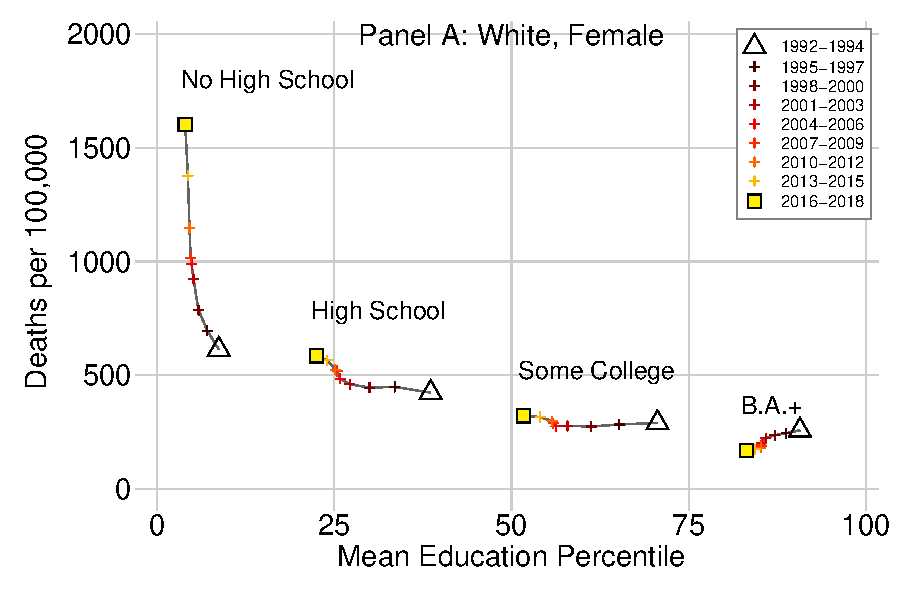
\includegraphics[scale=.6]{\mortalitypath/scatter-smooth-t-50-2-1}
    & 
    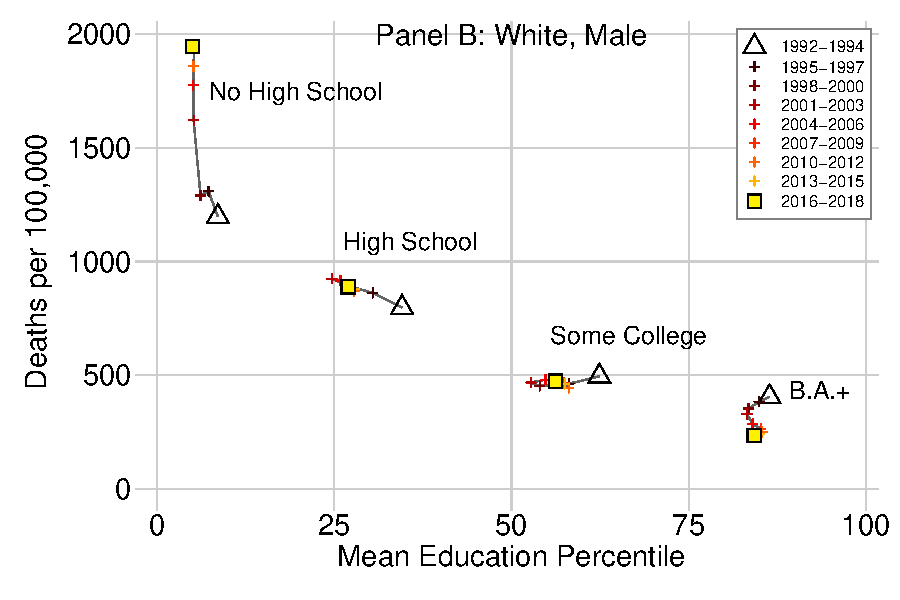
\includegraphics[scale=.6]{\mortalitypath/scatter-smooth-t-50-1-1}
    \\
    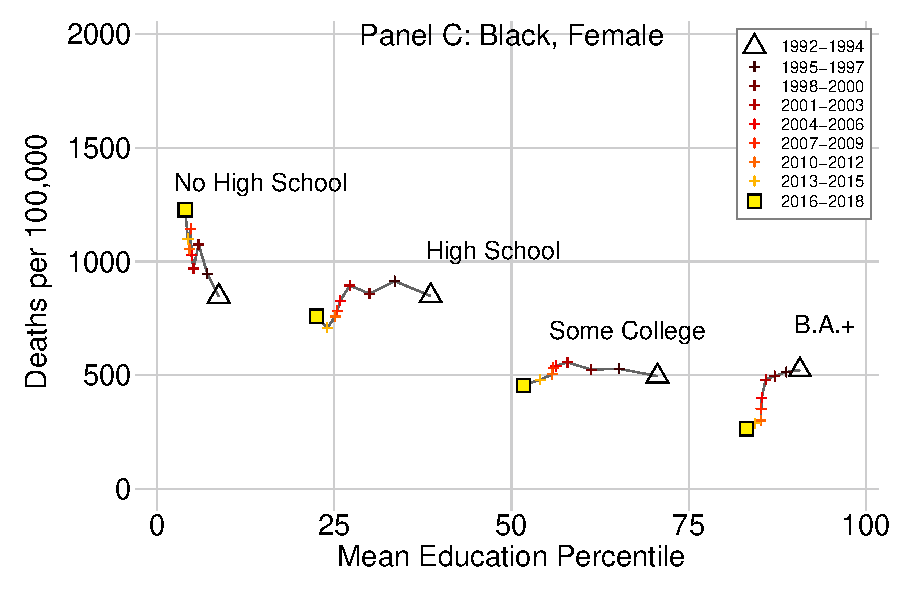
\includegraphics[scale=.6]{\mortalitypath/scatter-smooth-t-50-2-2}
    & 
    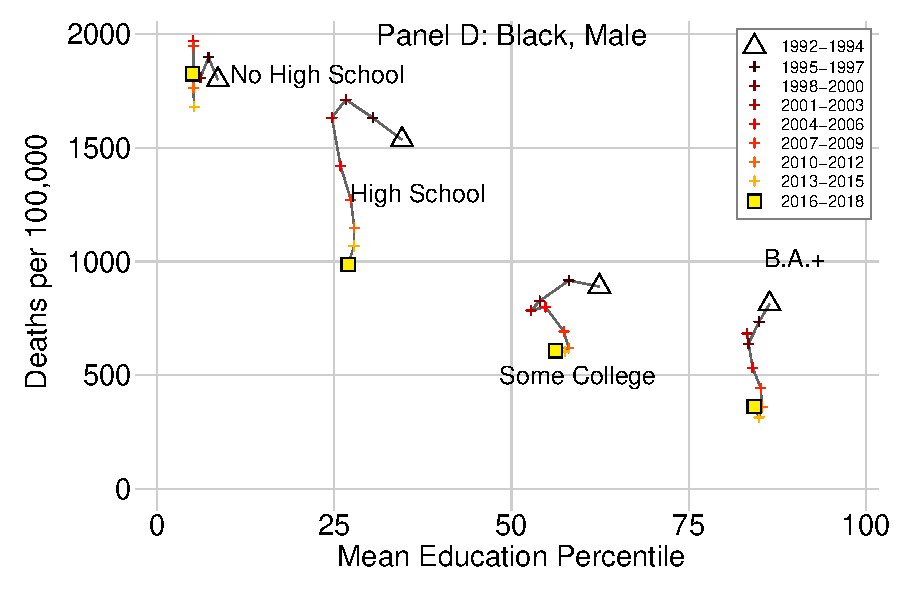
\includegraphics[scale=.6]{\mortalitypath/scatter-smooth-t-50-1-2}
    \end{tabular}
  \end{center}
    \footnotesize{Note: ``White'' refers to non-Hispanic white and
      ``Black'' to non-Hispanic black. The figure shows change in
      mortality and average education rank for individuals aged 50--54
      at different levels of education, from 1992--1994 to 2016--2018. Each point
      represents the average number of deaths per 100,000 people among
      people with one of four levels of education: No High School,
      High School, Some College, and a B.A. or Higher. The $X$
      coordinate of each point represents the average education
      percentile among people with the given level of educational
      completion. For example, a 50-year-old white woman with a high school
      education was at the 39th percentile of the education
      distribution in 1992--1994 and at the 22nd percentile in
      2016--2018. Sources: ACS, CPS, NCHS.}
\end{figure}
\end{landscape}

%%%%%%%%%%%%%%%%%%%%%%%%%%%%%%%%%%%%%
%% INTUITIVE MU-BOUNDS EXPLANATION %%
%%%%%%%%%%%%%%%%%%%%%%%%%%%%%%%%%%%%%
\begin{figure}[H]
\thispagestyle{empty} 
  \caption{Calculating the CEF of Mortality Given Education Rank}
  \label{fig:intuit}
  \begin{center}
    \begin{tabular}{c}
      
      \panel{Panel A} \\
      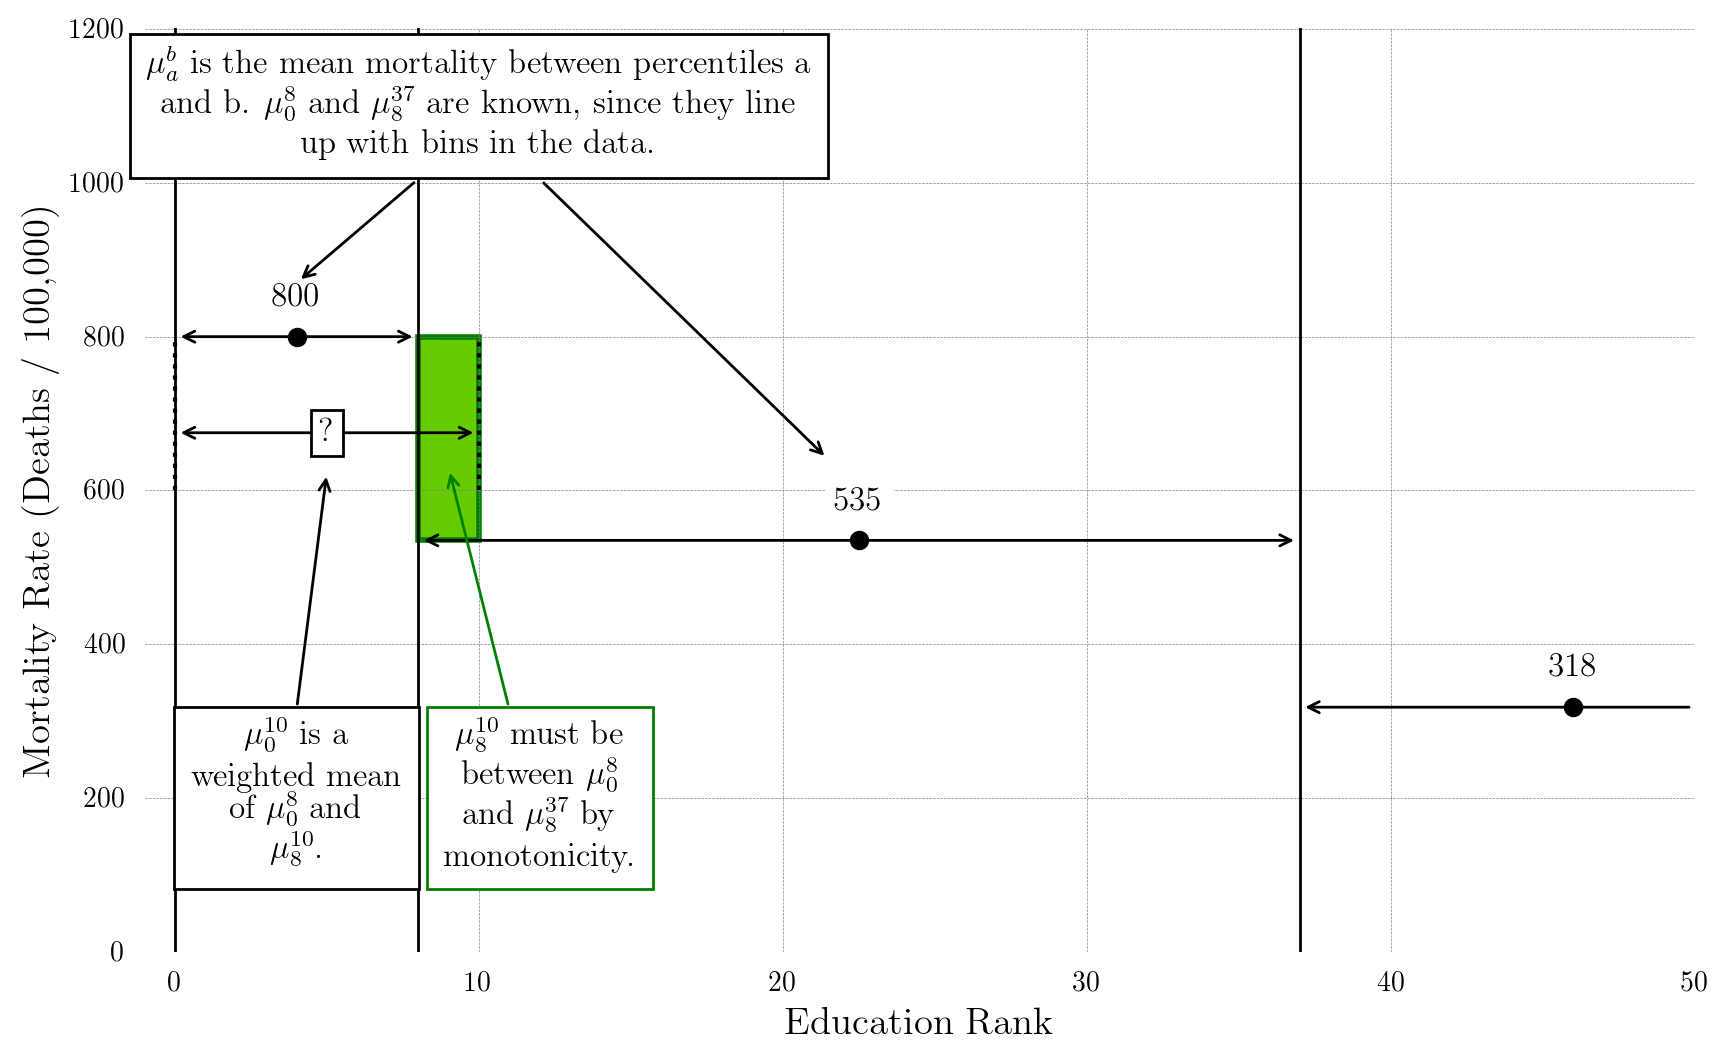
\includegraphics[scale=0.75]{\mortalitypath/intuit_a} \\
      
      \panel{Panel B} \\
      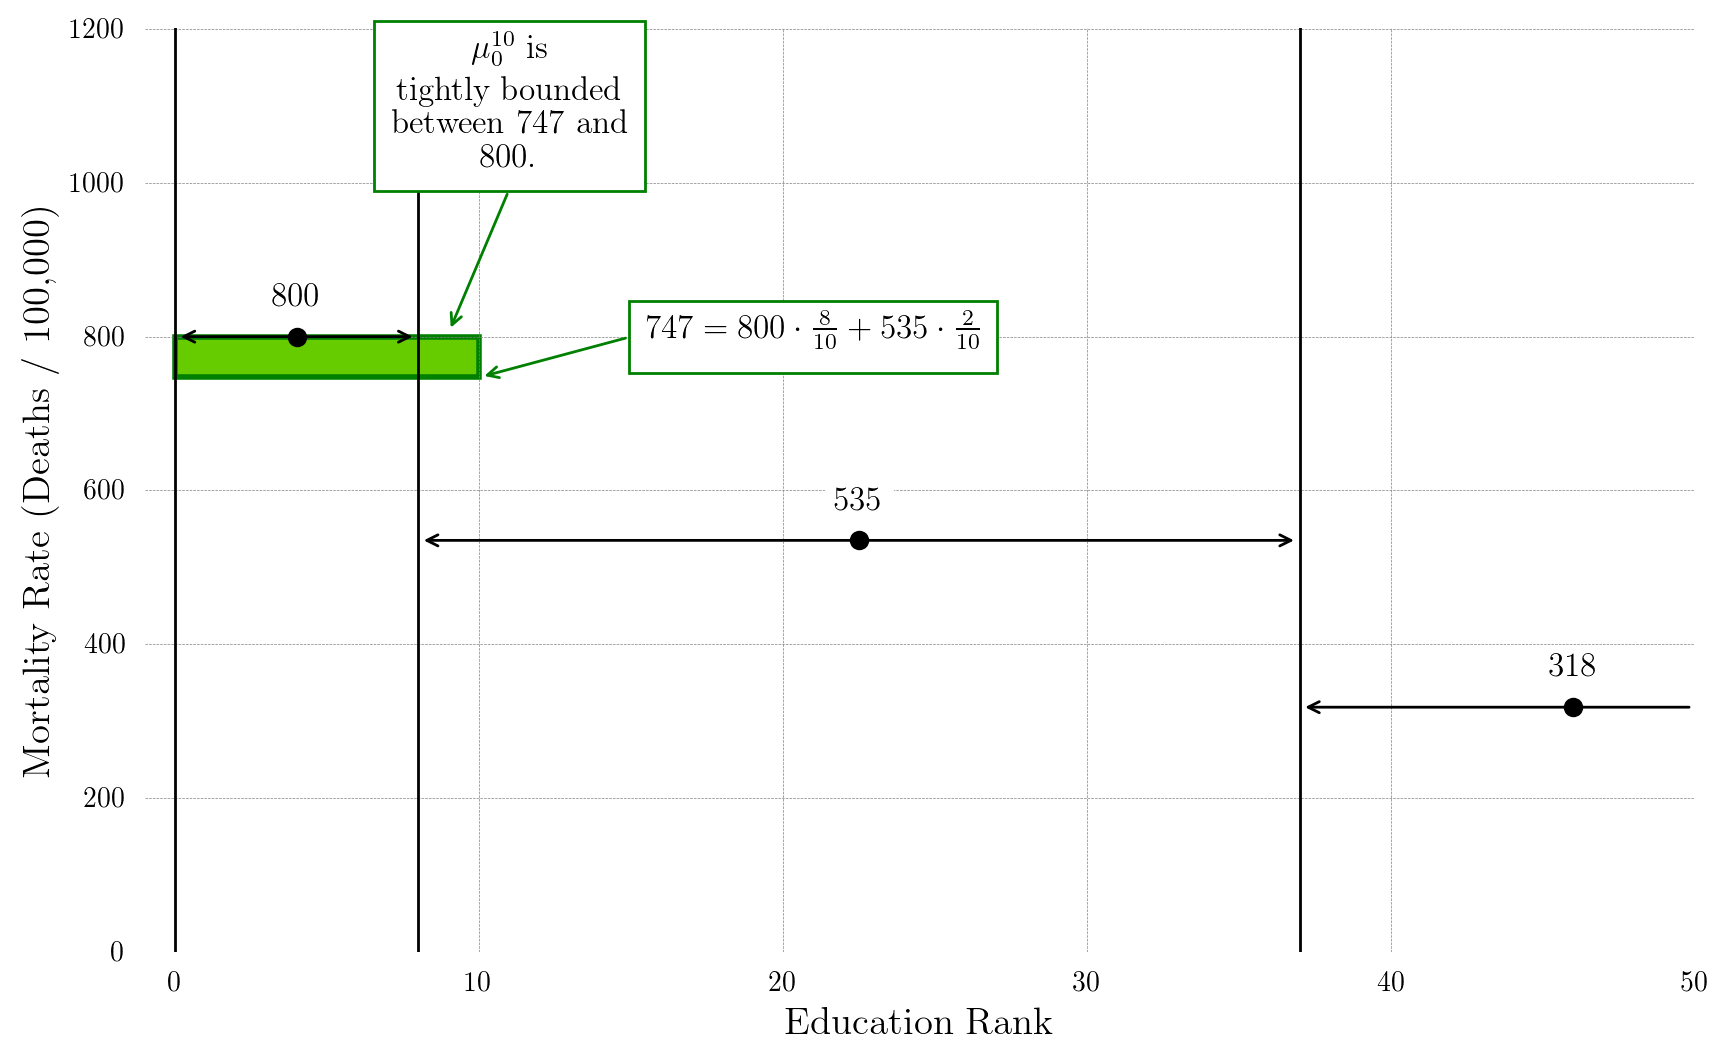
\includegraphics[scale=0.75]{\mortalitypath/intuit_b} \\
      
    \end{tabular}
  \end{center}
\end{figure}

\begin{figure}[H]\ContinuedFloat
\thispagestyle{empty} 
  \begin{center}
    \begin{tabular}{c}

      \panel{Panel C} \\
      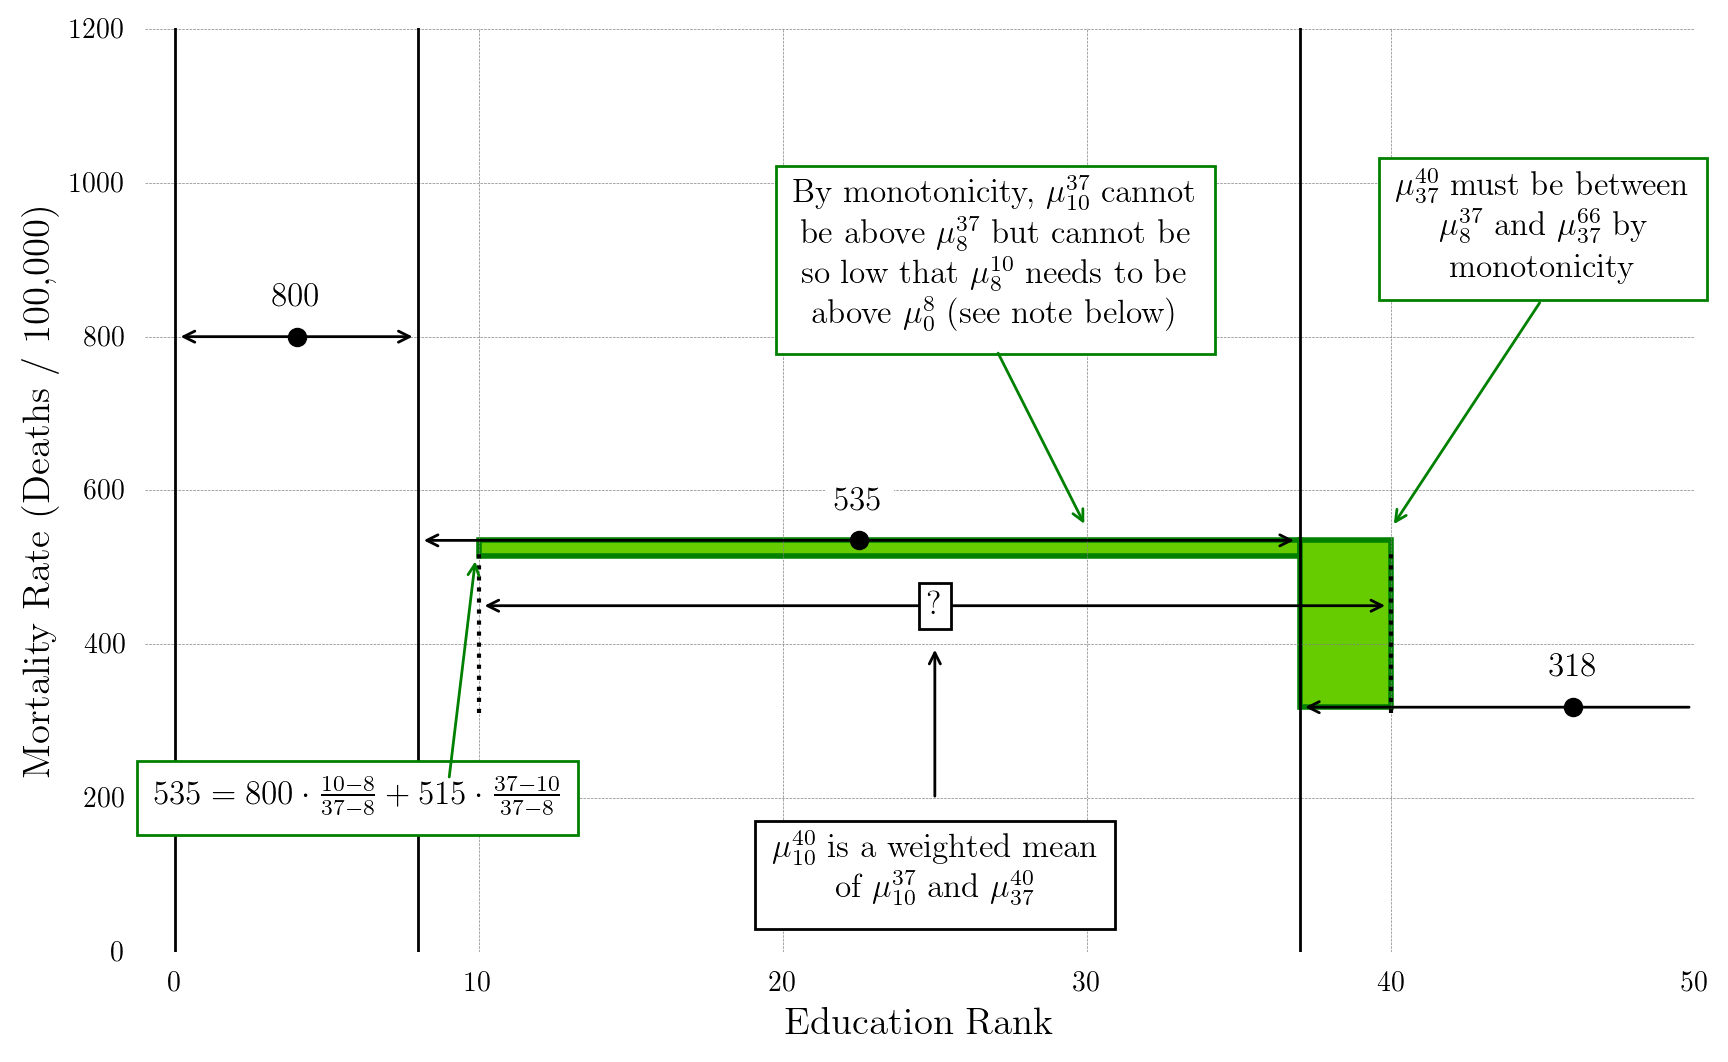
\includegraphics[scale=0.75]{\mortalitypath/intuit_c} \\
      
      \panel{Panel D} \\
      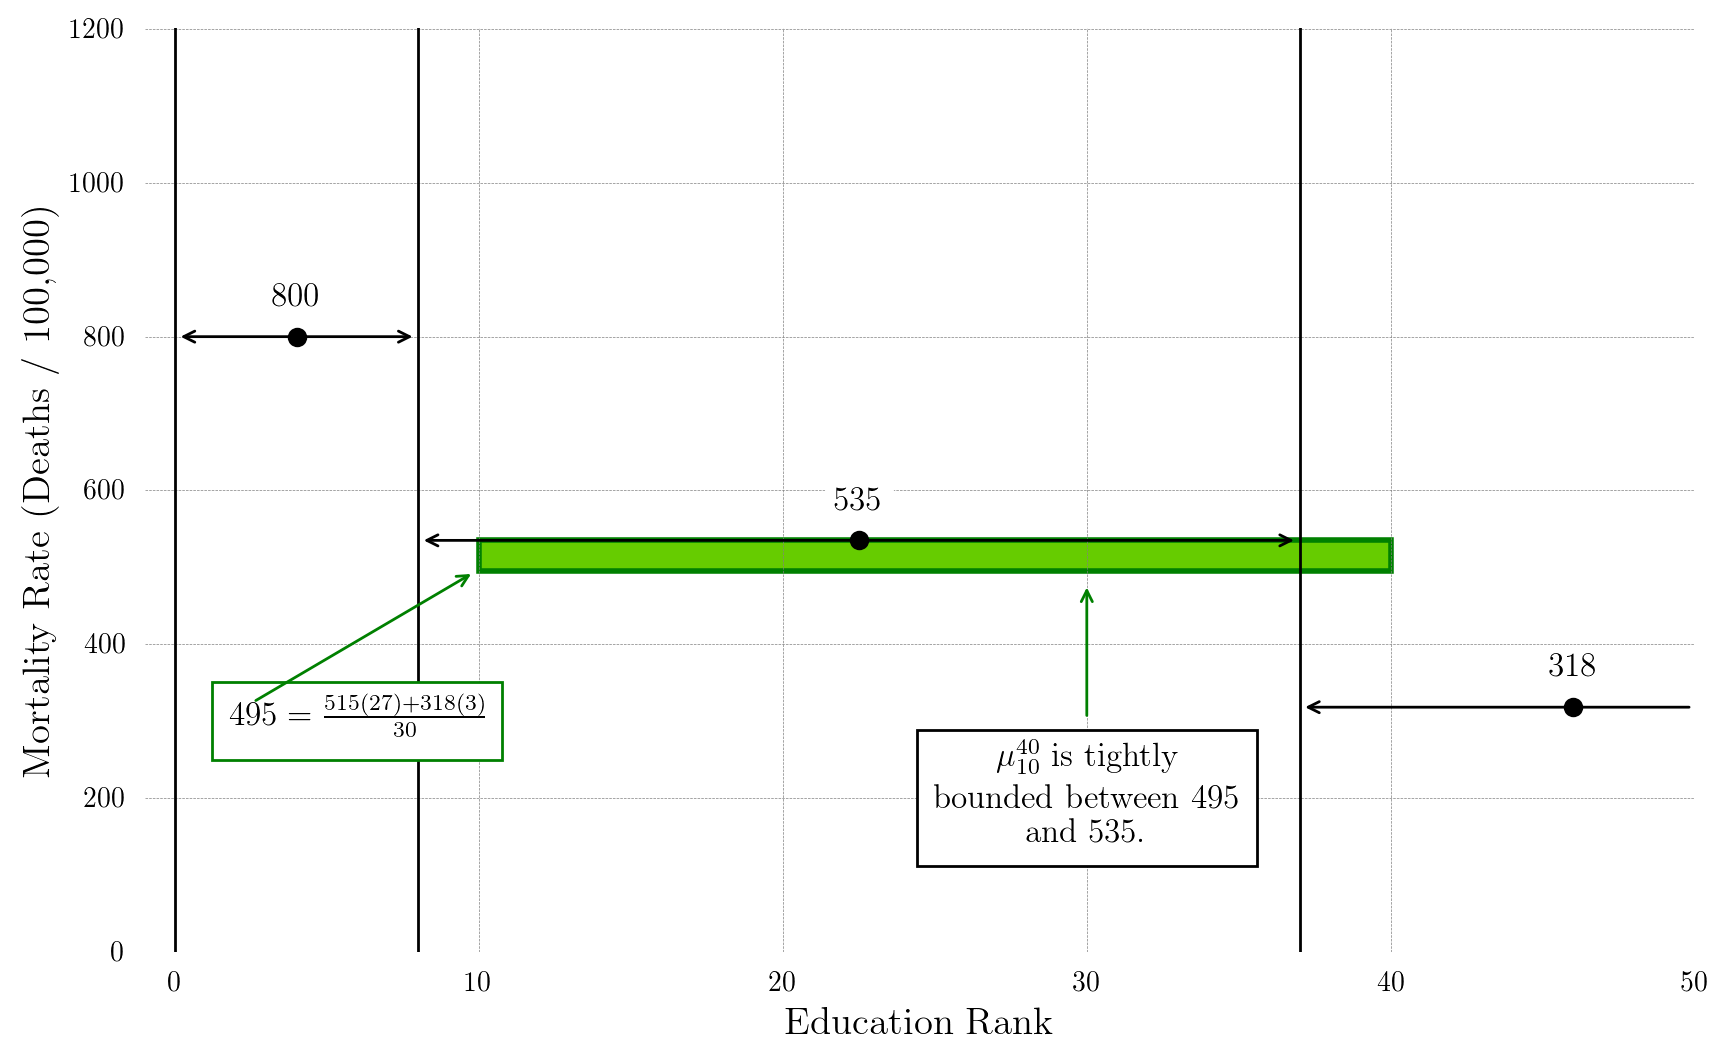
\includegraphics[scale=0.75]{\mortalitypath/intuit_d} \\
      \hline
    
    \end{tabular}
  \end{center}
  \noindent
\thisfloatpagestyle{empty} 
  \footnotesize{Figure \ref{fig:intuit} provides a graphical description of the calculation of the bounds on $\mu_a^b$ in two scenarios. The data are from women aged 50--54 in 2016--18. The vertical lines show the rank bin boundaries for each education bin for this group. The points show the mean mortality in each bin. The first two panels show the calculation of $\mu_0^{10}$ and the following two panels show the calculation of $\mu_{10}^{40}$. In Panel C, the upper bound of $\mu_{10}^{37}$ cannot exceed the value of $\mu_8^{37}$, because that would require $\mu_8^{10} > \mu_{10}^{37}$. The lower bound cannot be below 514, or else $\mu_8^{10}$ would need to be higher than $\mu_0^8$ to fit the bin mean, thus violating monotonicity. Source: NCHS.}
\end{figure}

%%%%%%%%%%%%%%%%%%%%%%%%%%%
%% MORTALITY CEF COMPARE %%
%%%%%%%%%%%%%%%%%%%%%%%%%%%
\begin{figure}[H]
\caption{Change in Total Mortality of U.S. Women, Age 50--54
  \cnewline Bounds on Conditional Expectation Functions}
\label{fig:mort_overlay}
\begin{center}
    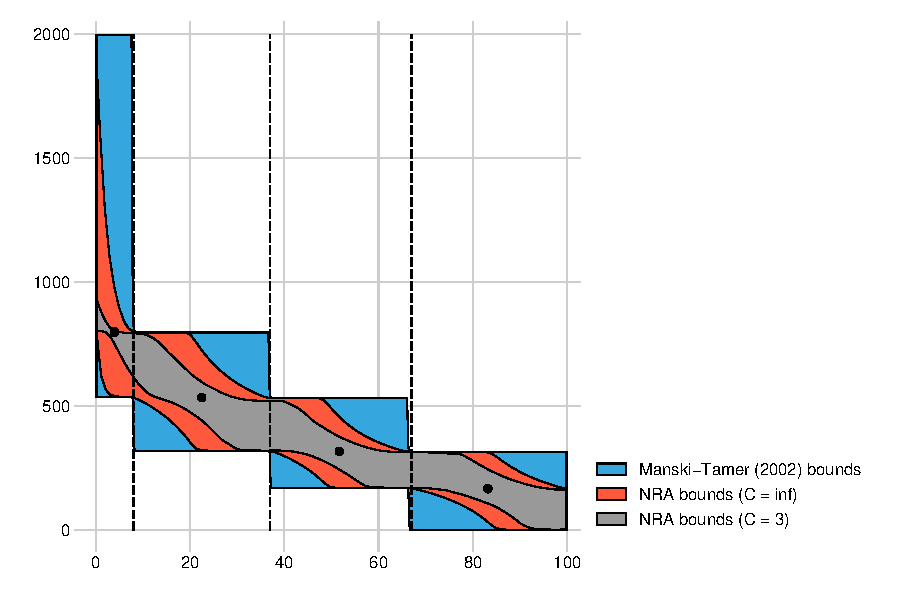
\includegraphics[scale=1.1]{\mortalitypath/mort_cef}
\end{center}
\noindent
\footnotesize{Figure \ref{fig:mort_overlay} shows bounds on the
  conditional expectation function of mortality as a function of
  latent educational rank. The sample consists of U.S. women aged
  50--54; mortality is measured in deaths per 100,000 women. The
  points in the graph show the mean education rank and mortality in
  each year for individuals with (i) less than high school; (ii) high
  school; (iii) some college; and (iv) a B.A. or higher. The curves
  show the bounds on expected mortality at each latent parent rank
  ($E(Y|X=i)$ in the text). The outer (blue) bounds are calculated
  following \cite{Manski2002}. In the bottom bin, the blue bounds are
  truncated at 2,000 for visual clarity but actually extend to 100,000
  (since the procedure cannot reject a mortality rate of 1 up to the
  first bin cut). The middle (red) bounds are calculated following our method with unrestricted curvature. The tightest (gray) bounds are calculated restricting the curvature to 3\% of mean mortality across every percentile bin (2x the largest curvature found in U.S. income rank-rank data \citep{Chetty2016b}.). Education rank is measured relative to the set of all women aged 50--54. Source: NCHS}

\end{figure}
 
%%%%%%%%%%%%%%%%%%%%%%%%%%%%%%%%%%%%%%%%
%% BIAS OF MORTALITY CHANGE ESTIMATES %%
%%%%%%%%%%%%%%%%%%%%%%%%%%%%%%%%%%%%%%%%
\begin{figure}[htbp]
\caption{Changes in U.S. Mortality, Age 50--54, 1992--94 to 2016--18:
  \cnewline Naive and Constant Rank Interval Estimates (Women, Ages 50--54)}
\label{fig:mort_bias}
\begin{center}

  \begin{tabular}{c}
    Panel A: Less than High School \\
    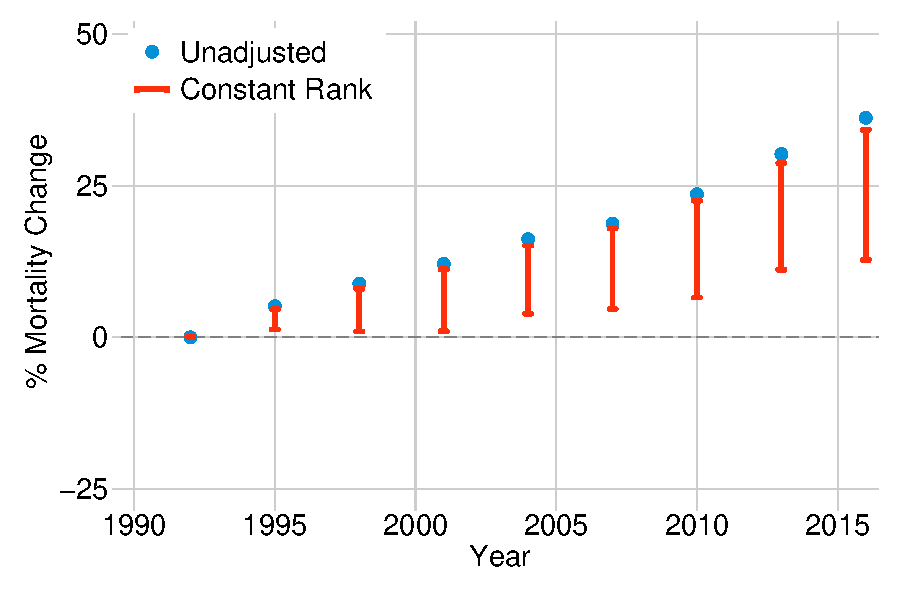
\includegraphics[scale=.8]{\mortalitypath/naive-5-women-50-t-1}
    \\
 Panel B: High School \\
    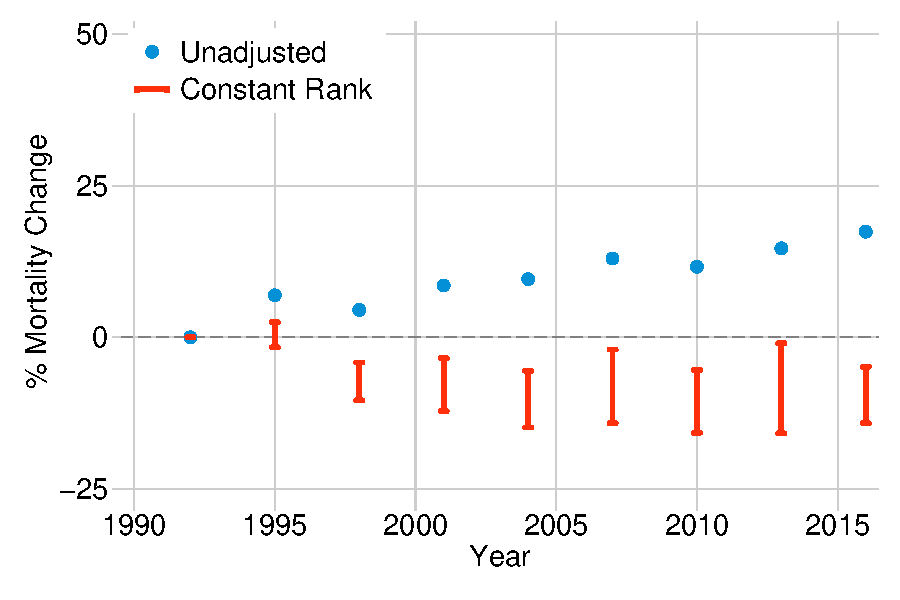
\includegraphics[scale=.8]{\mortalitypath/naive-5-women-50-t-2} \\
    \hline
  \end{tabular}
\end{center}
\noindent
Figure~\ref{fig:mort_bias} shows mortality changes for 50--54-year-old women from 1992--94 to 2016--18 (all races combined), calculated under different methods. The points show unadjusted estimates for women at constant education levels---dropouts in Panel A and high school graduates in Panel B. Both of these population groups have shrunk as proportions of the population during the sample period. The vertical bars show bounds on mortality change in constant rank bins---ranks 0--17 in Panel A and ranks 17--60 in Panel B. These ranks are chosen because they are close to the share of women in 1992--1994 with less than a high-school degree or exactly a high school degree, allowing the bounds to be very tight in the starting period.
\end{figure}

%%%%%%%%%%%%%%%%%%%%%%%%%%%%%%%%%%%%%
%% BOUNDED MORTALITY TRENDS BY GROUP
%%%%%%%%%%%%%%%%%%%%%%%%%%%%%%%%%%%%%
\begin{figure}[H]
  \floatpagestyle{empty}
    \caption{All-Cause Mortality Change in Constant Education
      Percentiles: \cnewline Age 50--54, 1992--1994 to 2016--2018}
    \label{fig:trend}
    \begin{center}
      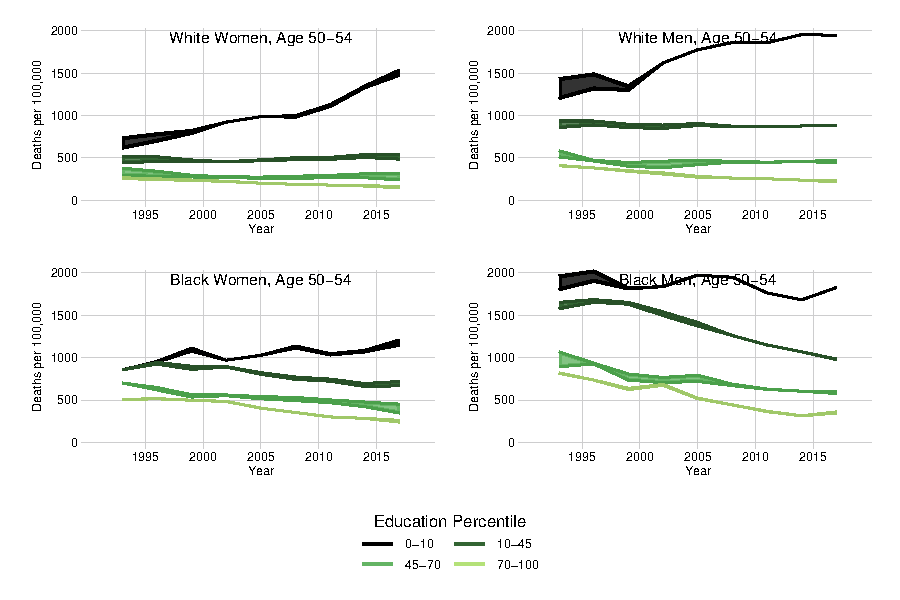
\includegraphics[scale=1.1]{\mortalitypath/trend-smooth-mon-step-t-sex-50}
    \end{center}
  \footnotesize{Note: ``White'' refers to non-Hispanic white and ``Black'' to non-Hispanic black.  Each interval represents the bounded set containing the number of deaths per 100,000 people in a given time period, among people in the education percentiles specified in the legend. The education percentiles correspond to the percentile bins describing four levels of education for the median age group in 2003: No High School, High School, Some College, and a B.A. or Higher. Bounds are computed as described in Section~\ref{sec:method}. The sample consists of people ages 50--54. Sources: ACS, CPS, NCHS.}
\end{figure}

%%%%%%%%%%%%%%%%%%%%%%%%%%%%%%%%%%%%%%%%%%%%%%%%%%%%%%%%%%%%%%%%
% Figure:      Main Mortality Estimates                        %
%              White Women, White Men, Black Women, Black Men  %
%%%%%%%%%%%%%%%%%%%%%%%%%%%%%%%%%%%%%%%%%%%%%%%%%%%%%%%%%%%%%%%%

\begin{figure}[H]
  \floatpagestyle{empty}
  \caption{Mortality Change in Constant Education
    Percentiles (1992--1994 to 2016--2018, All Ages)}
  \label{fig:mort_main}
  \begin{center}
    \begin{tabular}{c}
      \panel{\textbf{A. Non-Hispanic White Women}} \\
      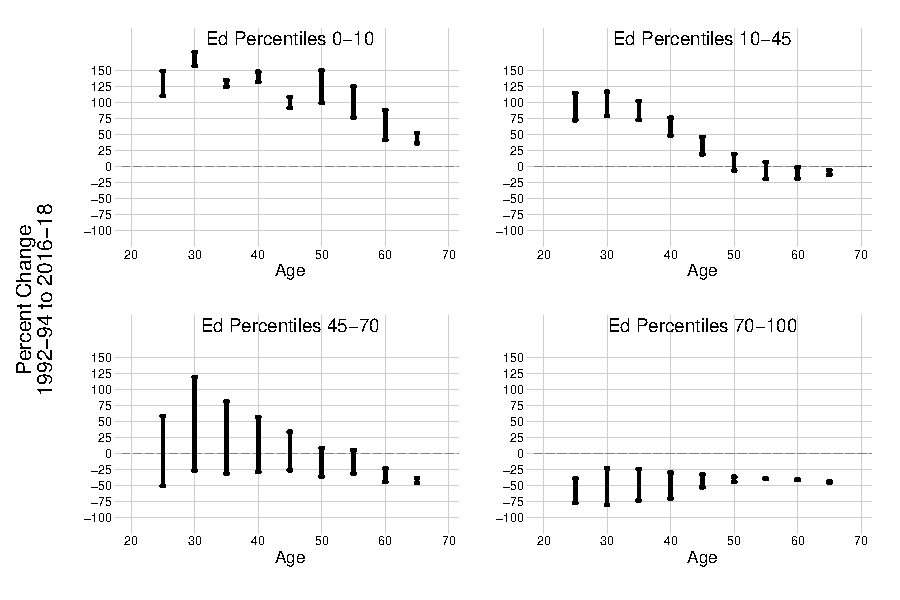
\includegraphics[scale=0.9]{\mortalitypath/changes-total-2-1} \\
      \panel{\textbf{B. Non-Hispanic White Men}} \\
      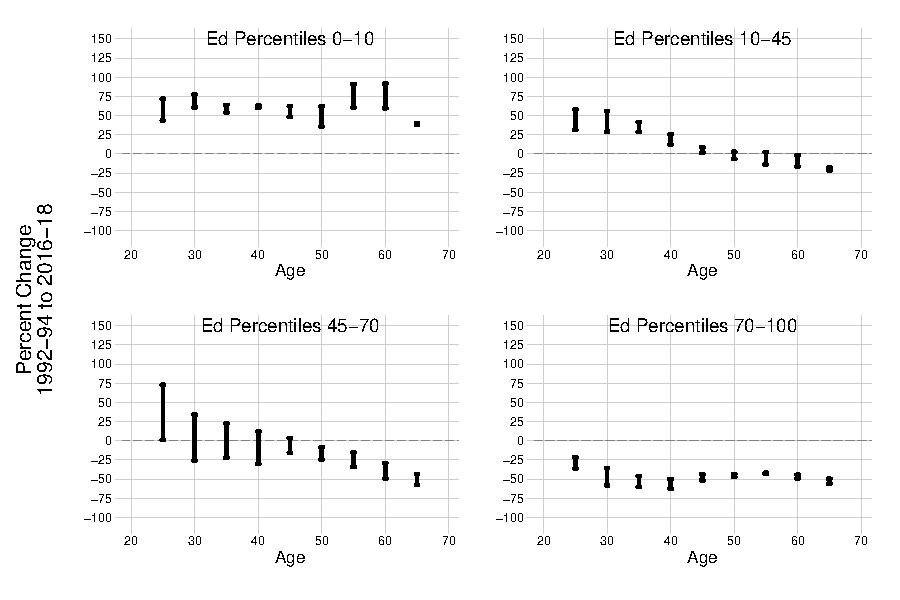
\includegraphics[scale=0.9]{\mortalitypath/changes-total-1-1} \\
    \end{tabular}
  \end{center}
  \vspace{-.5cm} \scriptsize{The graph shows changes in mortality by age, sex, race, and
    constant percentile education bin. The vertical lines show the
    bounded set containing the percentage change in the mortality rate
    from 1992--1994 to 2016--2018 for the given age group. Bounds are
    computed as described in Section~\ref{sec:method}. Sources: ACS, CPS, NCHS.}
\end{figure}
\begin{figure}[H]\ContinuedFloat
  \begin{center}
    \begin{tabular}{c}    
      \panel{\textbf{C. Non-Hispanic Black Women}} \\
      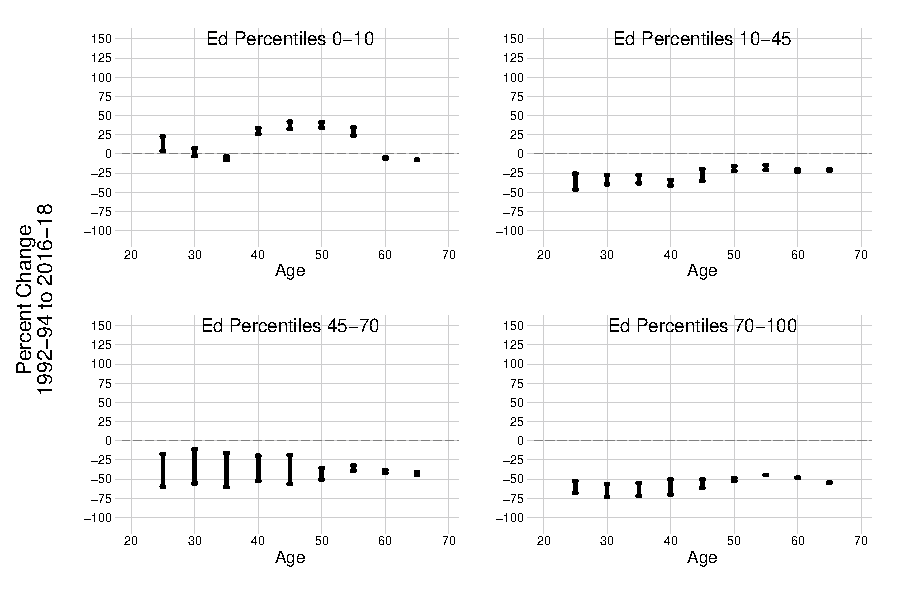
\includegraphics[scale=0.9]{\mortalitypath/changes-total-2-2} \\
      \panel{\textbf{D. Non-Hispanic Black Men}} \\
      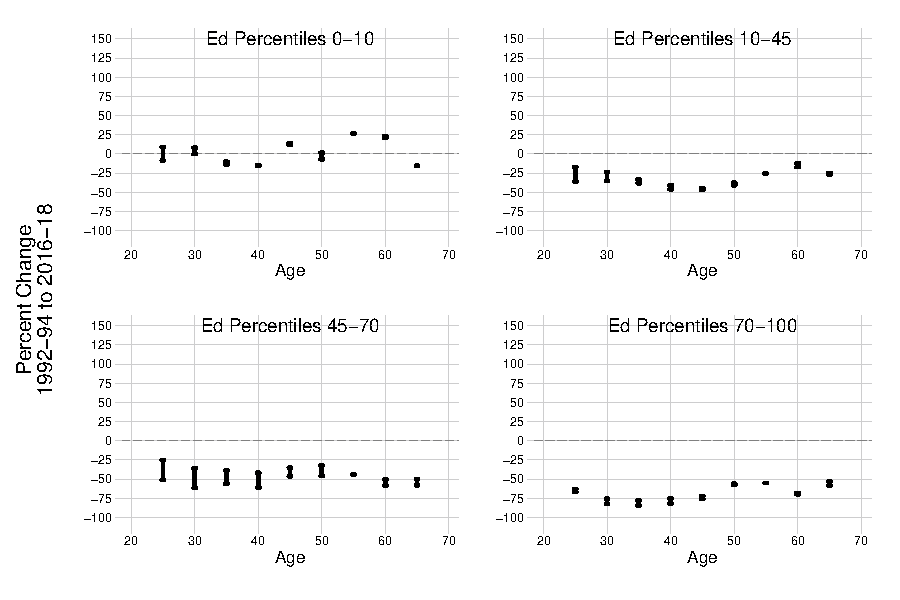
\includegraphics[scale=0.9]{\mortalitypath/changes-total-1-2} \\
    \end{tabular}
  \end{center}
  \vspace{-.5cm} \scriptsize{Note: The graph shows changes in
    mortality by age, sex, race, and constant percentile education bin. The vertical lines show the bounded set containing the percentage change in the mortality rate
    from 1992--1994 to 2016--2018 for the given age group. Bounds are
    computed using the set identification methods described in
    Section~\ref{sec:method}. Sources: ACS, CPS, NCHS.}
\end{figure}

%%%%%%%%%%%%%%%%%%%%%%%%%%%%%%%%%%%%%%%%%%%%%%%%%%%%%%%%%%%
%% FIGURE: CHANGES BY GROUP WITH ALL CAUSES OF MORTALITY %%
%%%%%%%%%%%%%%%%%%%%%%%%%%%%%%%%%%%%%%%%%%%%%%%%%%%%%%%%%%%
\begin{figure}[H]
  \caption{Decomposition of Mortality Change from 1992--94 to 2016--18: \cnewline
    Contribution of Deaths of Despair}
  \label{fig:mort_causes}

  \begin{center}
    \panel{\textbf{A. Non-Hispanic White Women}} \\
  \end{center}
  \begin{center}
    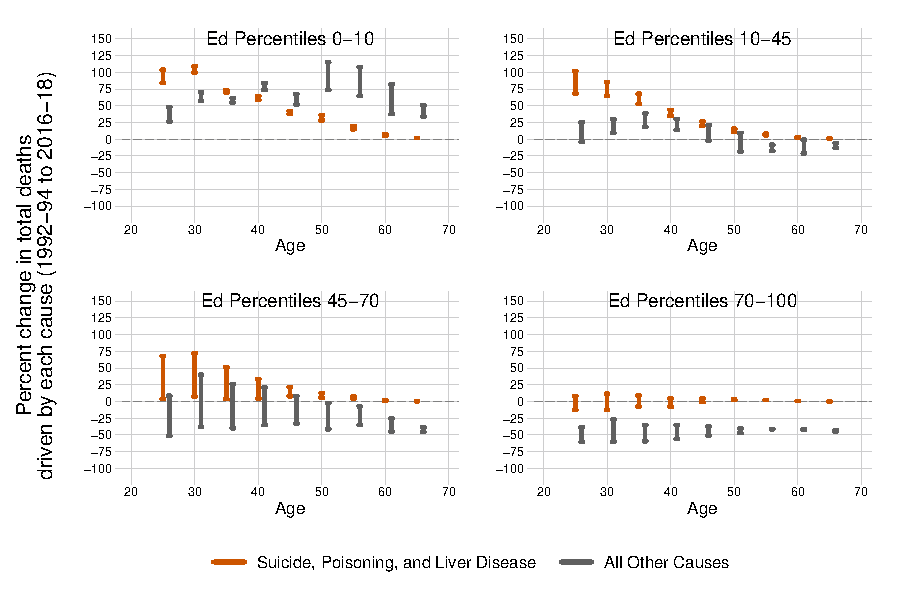
\includegraphics[scale=0.9]{\mortalitypath/changes-nod-2-1} &
  \end{center}

  \begin{center}
    \panel{\textbf{B. Non-Hispanic White Men}} \\
  \end{center}
  \begin{center}
    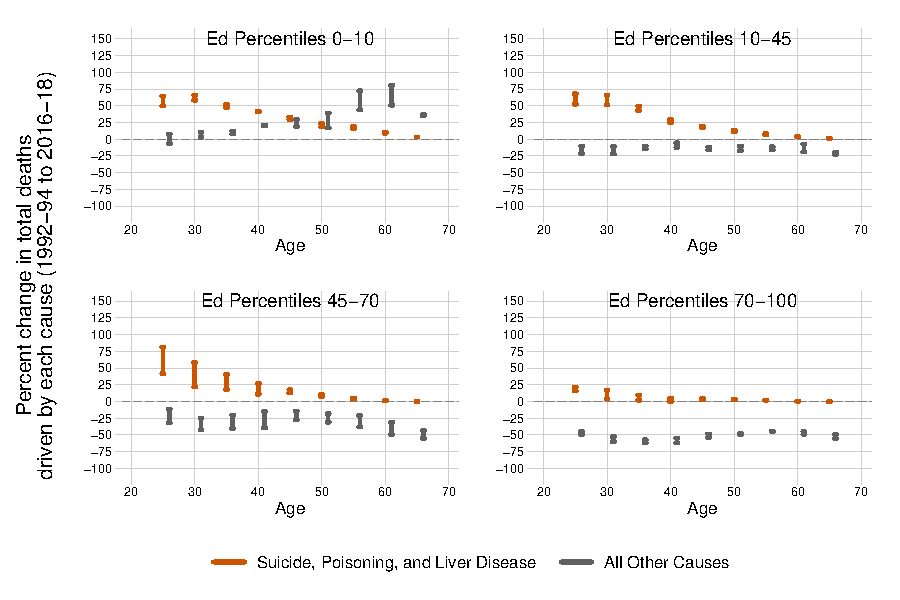
\includegraphics[scale=0.9]{\mortalitypath/changes-nod-1-1} \\
  \end{center}
\end{figure}
\begin{figure}[H]\ContinuedFloat

  \begin{center}
    \panel{\textbf{C. Non-Hispanic Black Women}} \\
  \end{center}
  \begin{center}
    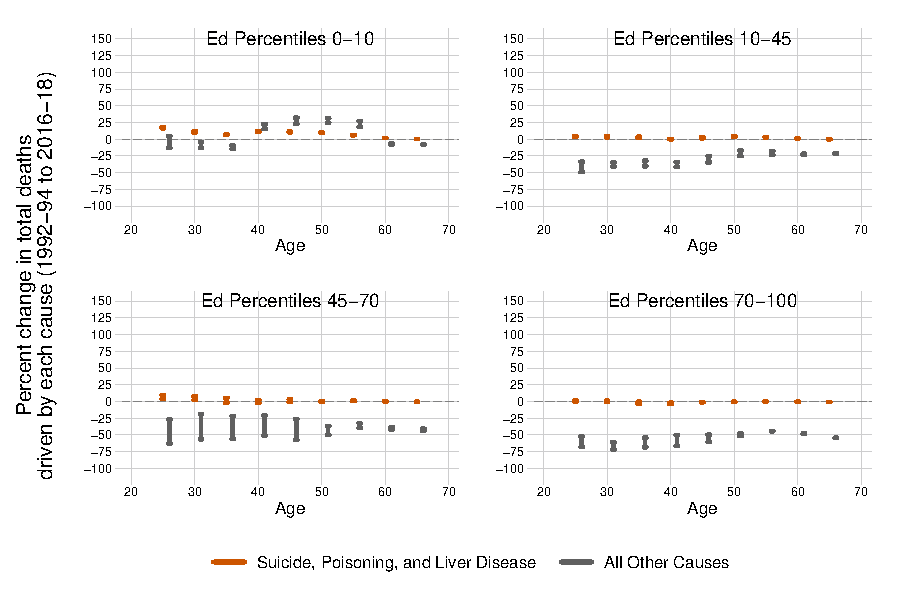
\includegraphics[scale=0.8]{\mortalitypath/changes-nod-2-2} &
  \end{center}
  \begin{center}
    \panel{\textbf{D. Non-Hispanic Black Men}} \\
  \end{center}
  \begin{center}
    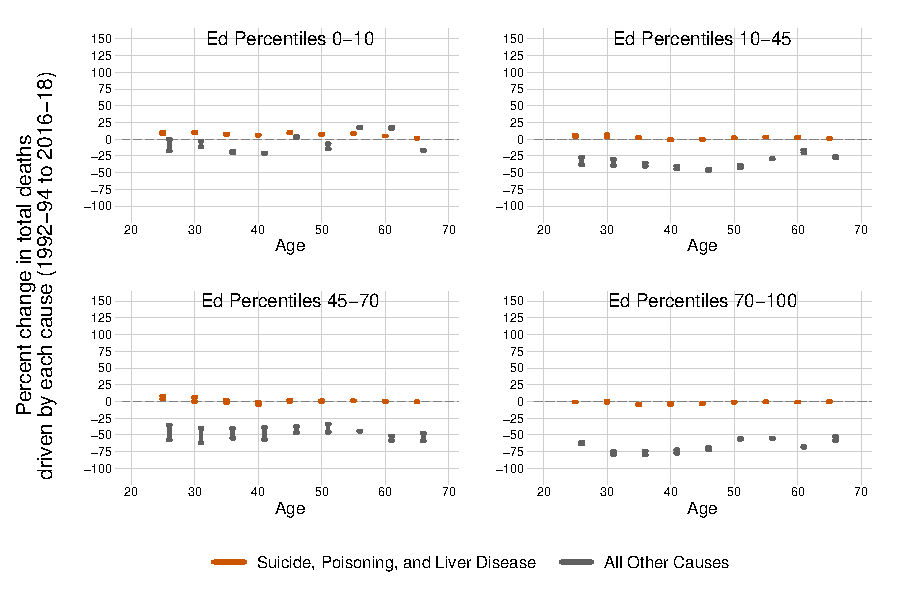
\includegraphics[scale=0.8]{\mortalitypath/changes-nod-1-2} \\
  \end{center}
\end{figure}
\vspace{-1cm}
\scriptsize{Note: ``White'' refers to non-Hispanic white. The graph decomposes the change in total mortality from 1992--1994 to 2016--2018 into two parts: the change in total deaths driven by deaths of despair, and the change in total deaths driven by all other causes. Estimates are disaggregated by age, sex, race, and constant percentile education bin. The orange lines show bounds on the contribution to total mortality change driven by changes in deaths of despair. The value on the $Y$ axis is the amount that total mortality for each group would have changed if the rates of all deaths \textit{other} than deaths of despair were unchanged. The gray lines show the contribution to total mortality change driven by all causes of death \textit{other} than deaths of despair. Deaths of despair are deaths from suicide, poisoning, and chronic liver disease. Bounds are computed using the set identification methods described in Section~\ref{sec:method}. Sources: ACS, CPS, NCHS.}

\floatbarrier
\clearpage
\begin{table}[H]
  \caption{Bounds on Mortality Thoughout the Education Rank Distribution \cnewline 50--54-Year-Old Women, All Races}
  \label{tab:bound_stats}
  \begin{center}
    \begin{tabular}{c}
      \panel{A. 1992--1994} \\

      \begin{tabular}{lccc}
\hline
Statistic                                    & Monotonicity Only                                 & Curvature Only                                            & Monotonicity and                                      \\
                                             & $(\overline{C}=\infty)$                           & $(\overline{C}=3)$                                        & Curvature $\overline{C}=3$                            \\
\hline
$Y(x=10)$: First Quintile Median              & [455.9, 682.1]   & [343.3, 793.8]   & [456.1, 614.7]   \\
$Y(x=25)$: Bottom Half Median                 & [427.7, 587.2]   & [0.0, 1163.1]   & [436.9, 586.7]   \\
$Y(x=8)$: Median $\le$ High School (1992--94)   & [455.9, 738.0]   & [453.1, 726.2]   & [485.9, 638.8]   \\
$Y(x=4)$: Median $\le$ High School (2016--18)   & [455.9, 1013.2]   & [263.6, 972.2]   & [573.1, 730.5]   \\
\rule{0pt}{2ex}                              &                                                   &                                                           &                                                       \\
$\mu_0^{20}$: First Quintile Mean            & [570.2, 587.2] & [539.0, 607.1] & [567.6, 586.2] \\
$\mu_0^{50}$: Bottom Half Mean               & [501.6, 530.7] & [431.3, 582.1] & [504.3, 529.5] \\
$\mu_0^{16}$: Mean $\le$ High School (1992--94) & [587.2, 598.7] & [585.3, 595.2] & [588.1, 595.1] \\
$\mu_0^{8}$: Mean $\le$ High School (2016--18) & [587.2, 741.5] & [259.7, 1041.2] & [587.5, 725.6] \\
\hline
\end{tabular}

 \\
      \\
      
      \panel{B. 2016--2018} \\
      
      \begin{tabular}{lccc}
\hline
Statistic                                    & Monotonicity Only                                 & Curvature Only                                            & Monotonicity and                                      \\
                                             & $(\overline{C}=\infty)$                           & $(\overline{C}=3)$                                        & Curvature $\overline{C}=3$                            \\
\hline
$Y(x=10)$: First Quintile Median              & [516.0, 799.9]   & [284.9, 1074.7]   & [534.3, 799.8]   \\
$Y(x=25)$: Bottom Half Median                 & [318.5, 685.4]   & [208.2, 775.5]   & [349.0, 600.5]   \\
$Y(x=8)$: Median $\le$ High School (1992--94)   & [535.3, 799.9]   & [417.0, 1009.8]   & [535.4, 799.8]   \\
$Y(x=4)$: Median $\le$ High School (2016--18)   & [535.3, 1046.3]   & [737.3, 831.1]   & [733.8, 816.3]   \\
\rule{0pt}{2ex}                              &                                                   &                                                           &                                                       \\
$\mu_0^{20}$: First Quintile Mean            & [640.1, 799.9] & [476.9, 903.0] & [641.2, 783.0] \\
$\mu_0^{50}$: Bottom Half Mean               & [520.8, 570.1] & [455.5, 553.0] & [521.3, 551.2] \\
$\mu_0^{16}$: Mean $\le$ High School (1992--94) & [666.2, 799.9] & [551.7, 952.2] & [667.7, 793.0] \\
$\mu_0^{8}$: Mean $\le$ High School (2016--18) & [797.2, 799.9] & [799.9, 799.9] & [799.9, 799.9] \\
\hline
\end{tabular}

 \\
      \hline
    \end{tabular}
\end{center}
\end{table}
\footnotesize{Note: ``White'' refers to non-Hispanic white and
  ``black'' refers to non-Hispanic black. The table shows bounds on
  mortality in 1992--94 (Panel A) and 2016--18 (Panel B) at various
  ranks or rank ranges in the education distribution. The notation $Y(x=i)=E(Y|x=i)$
  describes mortality at education percentile $i$, and $\mu_a^b$
  describes average mortality between education percentiles $a$ and
  $b$. $\overline{C}$ is the maximum percentage change in mortality
  function curvature allowed in any one percentile that does not
  correspond to an education bin boundary. Sources: ACS, CPS, and NCHS}


\begin{table}[H]
  \caption{Age-Adjusted Changes in All-Cause Mortality \cnewline by Education Percentile, 1992--94 to 2016--18}
  \label{tab:mort_changes}
  \begin{center}
    \begin{tabular}{lcccc}
  \hline
              & \multicolumn{4}{p}{Education Percentile Group} \\
  \hline
              & 0--10th    & 10th--45th & 45th--70th & 70th--100th \\
  \hline
  White Women & (+77\%, +111\%) & (-0\%, +21\%) & (-39\%, -4\%) & (-48\%, -39\%)  \\
  White Men   & (+50\%, +68\%) & (-6\%, +5\%) & (-40\%, -18\%) & (-52\%, -45\%)  \\
  Black Women & (+11\%, +17\%) & (-28\%, -21\%) & (-47\%, -33\%) & (-55\%, -51\%)  \\
  Black Men   & (-0\%, +3\%) & (-33\%, -29\%) & (-54\%, -44\%) & (-67\%, -64\%)  \\
  
  \hline
\end{tabular}

\end{center}
\end{table}
\footnotesize{Note: ``White'' refers to non-Hispanic white and
  ``black'' refers to non-Hispanic black. The table shows the percent
  change in all-cause mortality, defined as total deaths in a year
  divided by population. To hold the population distribution constant,
  we weight the age-specific mortality rates from the data with the
  standardized U.S. population distribution for ages 25--69. We use
  age-specific mortality rates from each period, but a single set of
  weights for all periods.}

\floatbarrier

%%%%%%%%%%%%%%%%%%%%%%%%%%%%%%%%%%%%%%%
%% BEGIN APPENDIX TABLES AND FIGURES %%
%%%%%%%%%%%%%%%%%%%%%%%%%%%%%%%%%%%%%%%
\newpage 
\renewcommand{\thetable}{A\arabic{table}}
\setcounter{table}{0}
\renewcommand{\thefigure}{A\arabic{figure}}
\setcounter{figure}{0}
\section{Appendix: Additional Tables and Figures} 
\label{sec:app_figs}
%%%%%%%%%%%%%%%%%%%%%%%%%%%%%%%%%%%%%%%%%%%%
%% TABLE: DISTRIBUTION OF DEATHS BY CAUSE %%
%%%%%%%%%%%%%%%%%%%%%%%%%%%%%%%%%%%%%%%%%%%%
\begin{table}[H]
  \caption{Distribution of Deaths by Cause, Ages 25--69 (2018)}
  \label{tab:icd_causes}
  \begin{tabular}{lc}
    Cause of Death & Share of Total Deaths \\
    \hline
    Cancer&28.28\\
Heart and other diseases of the circulatory system&21.75\\
Poisoning, suicide, chronic liver disease ("deaths of despair") &11.82\\
Diseases of the respiratory system&8.00\\
Accidents and injuries (primarily falls, motor vehicles, assaults)&5.79\\
Endocrine, nutritional and metabolic diseases&5.36\\
Diseases of the nervous system&3.69\\
Cerebrovascular diseases&3.33\\
Infectious and parasitic diseases&2.72\\
Diseases of the digestive system&2.48\\
Diseases of the genitourinary system&1.95\\
Mental and behavioural disorders&1.92\\
Deaths not elsewhere classified&0.95\\
Diseases of the blood and immune disorders&0.88\\
Diseases of the musculoskeletal system and connective tissue&0.53\\
Congenital malformations, deformations and chromosomal abnormalities&0.27\\
Diseases of the skin and subcutaneous tissue&0.19\\
Pregnancy, childbirth and the puerperium&0.07\\
Diseases of the eye, ear, mastoid and adnexa&0.01\\
Certain conditions originating in the perinatal period&0.00\\

    \hline
  \end{tabular}
  \footnotesize{Note: The table shows the distribution of causes of
    death for individuals aged 25--69 in 2018. Categories are defined
    by major headings in the ICD-10 Cause-Of-Death lists. The
    categories of cancer, heart disease and deaths of despair are
    pooled across subcategories following the previous literature. See
    Appendix~\ref{sec:app_data} for additional details.}
\end{table}

%%%%%%%%%%%%%%%%%%%%%%%%%%%%%%%%%%%%%%%%%%%%%%%%%%%%%%
%% TABLE: AGE-ADJUSTED MORTALITY CHANGES, BY CAUSES %%
%%%%%%%%%%%%%%%%%%%%%%%%%%%%%%%%%%%%%%%%%%%%%%%%%%%%%%
\begin{landscape}
  \begin{table}[htbp]
    \caption{Age-Adjusted Changes in Mortality by
      Education Percentile and Cause \cnewline Ages 25--69, 1992--1994
      to 2016--2018}
    \label{tab:all_cause_all_age}
    \centering
\resizebox{\columnwidth}{!}{%
  \begin{tabular}{llcccccc}
  & & Injuries & Cancer & Heart Disease & Despair & Other & Total \\
  \hline
  \textbf{White non-Hispanic Women} & & & & & & & \\
  Education Percentile &  0--10  & (+62\%, +79\%) & (+25\%, +35\%) & (+3\%, +38\%) & (+526\%, +585\%) & (+111\%, +167\%) & (+77\%, +111\%) \\
                       & 10--45  & (+15\%, +36\%) & (-26\%, -18\%) & (-38\%, -16\%) & (+274\%, +354\%) & (+18\%, +52\%) & (-0\%, +21\%) \\
                       & 45--70  & (-29\%, +21\%) & (-48\%, -37\%) & (-59\%, -28\%) & (+64\%, +225\%) & (-26\%, +26\%) & (-39\%, -4\%) \\
                       & 70--100 & (-50\%, -34\%) & (-49\%, -47\%) & (-61\%, -55\%) & (-14\%, +42\%) & (-38\%, -28\%) & (-48\%, -39\%) \\

  \hline
  \textbf{White non-Hispanic Men} & & & & & & & \\
  Education Percentile &  0--10  & (+32\%, +47\%) & (+17\%, +27\%) & (+1\%, +13\%) & (+241\%, +267\%) & (+70\%, +102\%) & (+50\%, +68\%) \\
                       & 10--45  & (+2\%, +16\%) & (-30\%, -24\%) & (-38\%, -31\%) & (+156\%, +186\%) & (+3\%, +16\%) & (-6\%, +5\%) \\
                       & 45--70  & (-22\%, +15\%) & (-52\%, -42\%) & (-58\%, -45\%) & (+78\%, +148\%) & (-36\%, -14\%) & (-40\%, -18\%) \\
                       & 70--100 & (-44\%, -35\%) & (-55\%, -52\%) & (-63\%, -59\%) & (+17\%, +39\%) & (-54\%, -48\%) & (-52\%, -45\%) \\

  \hline
  \textbf{Black non-Hispanic Women} & & & & & & & \\
  Education Percentile &  0--10  & (+11\%, +19\%) & (-9\%, -6\%) & (-16\%, -11\%) & (+152\%, +168\%) & (+23\%, +32\%) & (+11\%, +17\%) \\
                       & 10--45  & (-33\%, -24\%) & (-31\%, -28\%) & (-42\%, -37\%) & (+44\%, +65\%) & (-21\%, -12\%) & (-28\%, -21\%) \\
                       & 45--70  & (-49\%, -25\%) & (-45\%, -40\%) & (-60\%, -49\%) & (-8\%, +48\%) & (-38\%, -20\%) & (-47\%, -33\%) \\
                       & 70--100 & (-60\%, -51\%) & (-49\%, -48\%) & (-67\%, -64\%) & (-41\%, -22\%) & (-51\%, -45\%) & (-55\%, -51\%) \\

  \hline
  \textbf{Black non-Hispanic Men} & & & & & & & \\
  Education Percentile &  0--10  & (+28\%, +39\%) & (-22\%, -19\%) & (-12\%, -10\%) & (+109\%, +118\%) & (-8\%, -4\%) & (-0\%, +3\%) \\
                       & 10--45  & (-18\%, -8\%) & (-46\%, -44\%) & (-37\%, -33\%) & (+30\%, +40\%) & (-36\%, -32\%) & (-33\%, -29\%) \\
                       & 45--70  & (-48\%, -21\%) & (-63\%, -57\%) & (-56\%, -49\%) & (-8\%, +22\%) & (-54\%, -45\%) & (-54\%, -44\%) \\
                       & 70--100 & (-69\%, -63\%) & (-68\%, -66\%) & (-66\%, -63\%) & (-45\%, -34\%) & (-69\%, -66\%) & (-67\%, -64\%) \\
\hline & & & & & & & \\
\end{tabular}
}

  \end{table}
  \footnotesize{ Note: The table shows age-adjusted percentage change
    in mortality from 1992--1994 to 2016--2018 for individuals aged 25
    to 69, by race, gender and education percentile bin. Each table
    entry shows the upper and lower bound on the percentage change in
    mortality over the sample period for the given cause and
    population subgroup. Ages are adjusted with a standardized
    U.S. population distribution, which holds constant that age
    distribution of the population across all years. Education
    percentile bins approximately describe the 2003 distribution of
    education across four categories: high schools dropouts
    (percentiles 0--10), high school graduates (10--45), some college
    (45--70) and B.A. or higher (70--100).}
\end{landscape}

%%%%%%%%%%%%%%%%%%%%%%%%%%%%%%%%%%%%%%%%%%%%%%%%%
%% FIGURE: BOUND ESTIMATES AND NAIVE ESTIMATES %%
%%%%%%%%%%%%%%%%%%%%%%%%%%%%%%%%%%%%%%%%%%%%%%%%%
\begin{figure}[H]
  \floatpagestyle{empty}
  \caption{Bounds on Constant Percentile Mortality Change and Naive
    Point Estimates \cnewline Age-Adjusted Populations, 1992--1994 to 2016--2018}
  \label{fig:bias}
  \begin{center}
    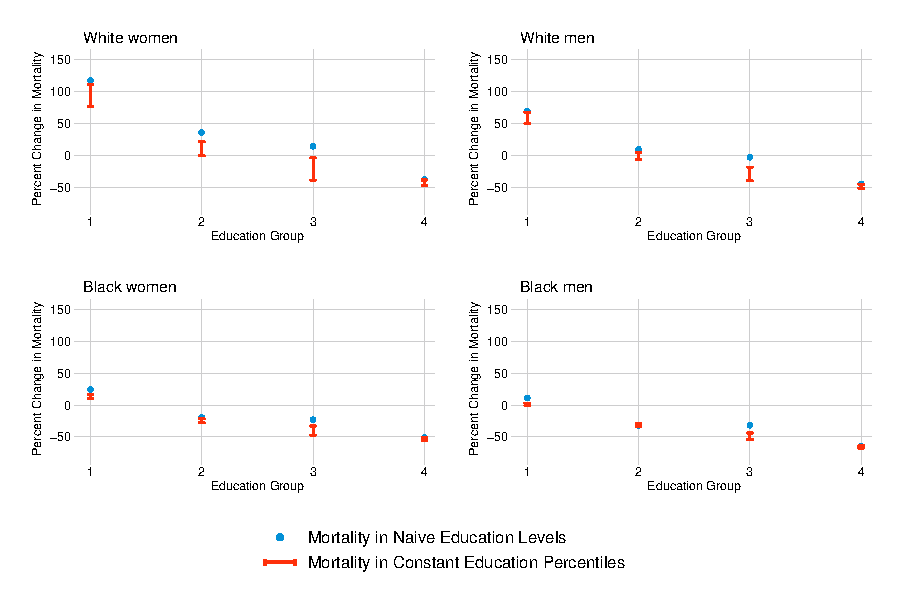
\includegraphics[scale=1.1]{\mortalitypath/std_mort_perc_total}
  \end{center}
  \footnotesize{Note: ``White'' refers to non-Hispanic white and
    ``Black'' to non-Hispanic black. The line segments in the graph
    show bounds on age-adjusted mortality change from 1992--1994 to
    2016--2018 for a standardized population, as in
    Table~\ref{tab:mort_changes}. The four education groups represent
    education percentiles (i) 0--10; (ii) 10--45; (iii) 45--70; and (iv) 70--100.
    The points in the graph show naive estimates of mortality rates at
    fixed education \textit{levels}; the four education levels for the
    points represent (i) high school dropouts; (ii) high school
    completers; (iii) some college; and (iv) a B.A. or higher.}
\end{figure}

%%%%%%%%%%%%%%%%%%%%%%%%%%%%%%%%%%%%%%%%%%%%%%%%%%%%%%%%%%%%%%%%%%%%%%%%
%% FIGURE: BOUND ESTIMATES AND NAIVE ESTIMATES -- ALL RACE-SEX GROUPS %%
%%%%%%%%%%%%%%%%%%%%%%%%%%%%%%%%%%%%%%%%%%%%%%%%%%%%%%%%%%%%%%%%%%%%%%%%
\begin{landscape}
\begin{figure}[H]
  \floatpagestyle{empty}
  \caption{Bounds on Constant Percentile Mortality Change and Naive
    Point Estimates: \cnewline 50--54-year-olds, 1992--1994 to 2016--2018}
  \label{fig:bias_more}
  \begin{center}
    \begin{tabular}{cc}
      \multicolumn{2}{c}{\textul{White Women}} \\
      Dropouts vs. p0--p17 & High School vs. p17--p60 \\
      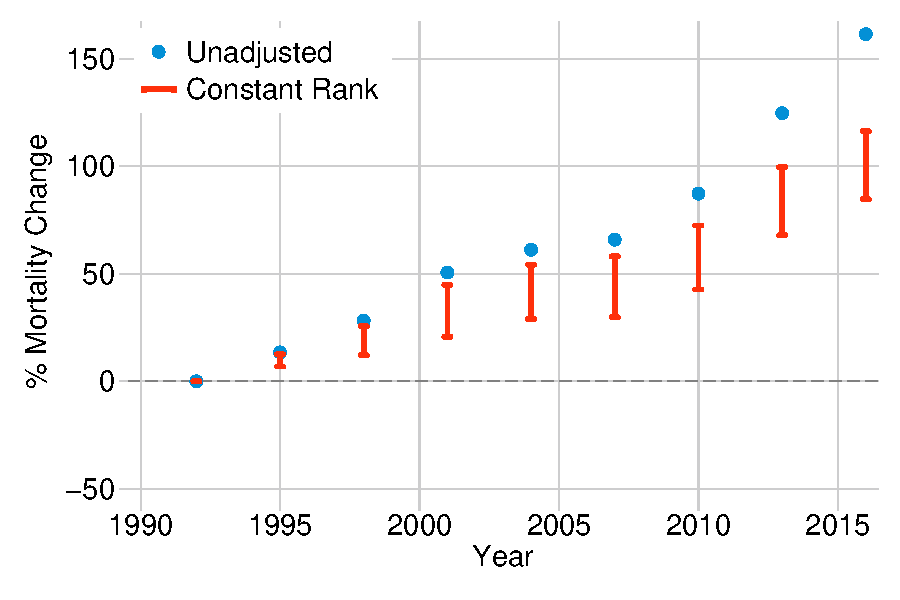
\includegraphics[scale=0.6]{\mortalitypath/naive-1-women-50-t-1} &
      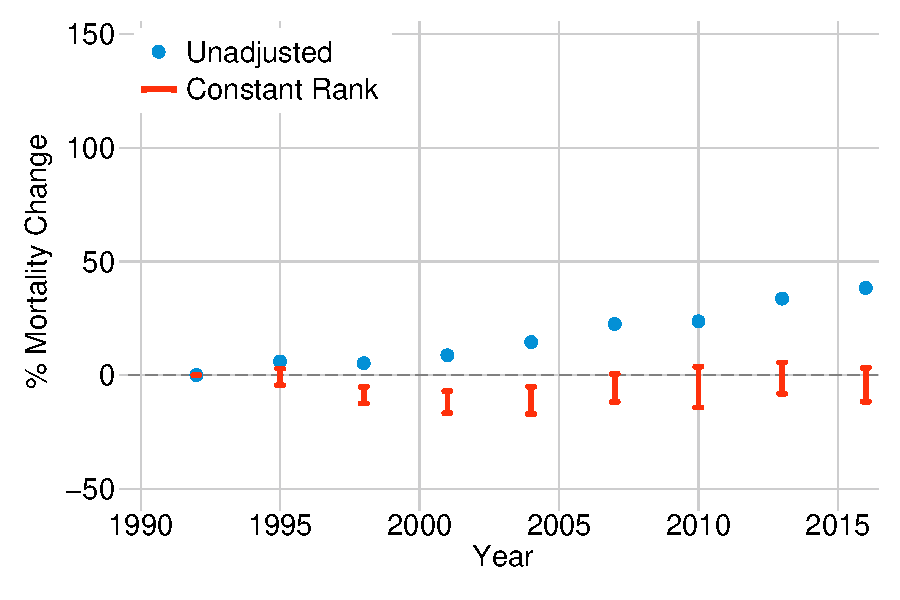
\includegraphics[scale=0.6]{\mortalitypath/naive-1-women-50-t-2} \\

      \multicolumn{2}{c}{\textul{White Men}} \\
      Dropouts vs. p0--p17 & High School vs. p17--p52 \\
      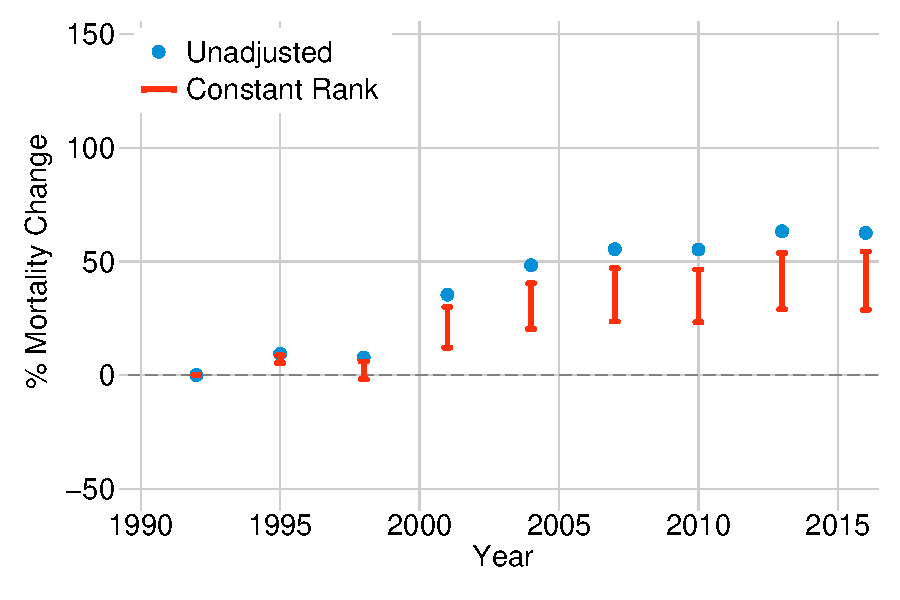
\includegraphics[scale=0.6]{\mortalitypath/naive-1-men-50-t-1} &
      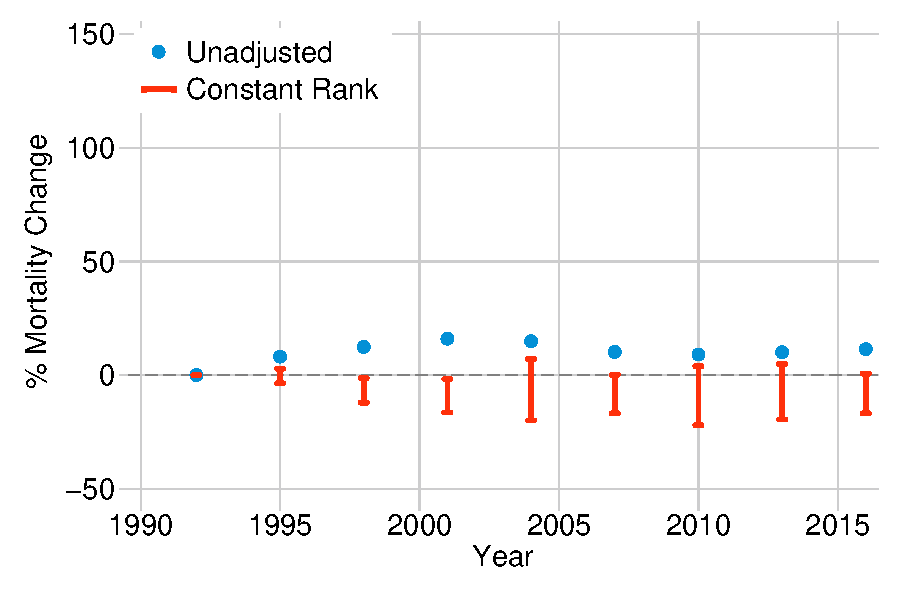
\includegraphics[scale=0.6]{\mortalitypath/naive-1-men-50-t-2} \\
      
    \end{tabular}
  \end{center}
  \end{figure}
\begin{figure}[H]\ContinuedFloat
  \begin{center}
    \begin{tabular}{cc}
      
      \multicolumn{2}{c}{\textul{Black Women}} \\
      Dropouts vs. p0--p17 & High School vs. p17--p60 \\
      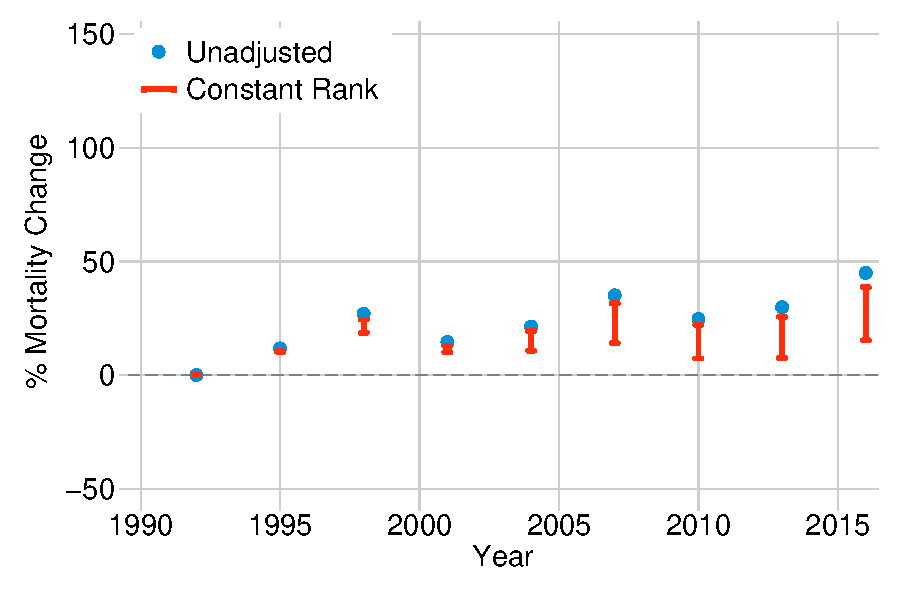
\includegraphics[scale=0.6]{\mortalitypath/naive-2-women-50-t-1} &
      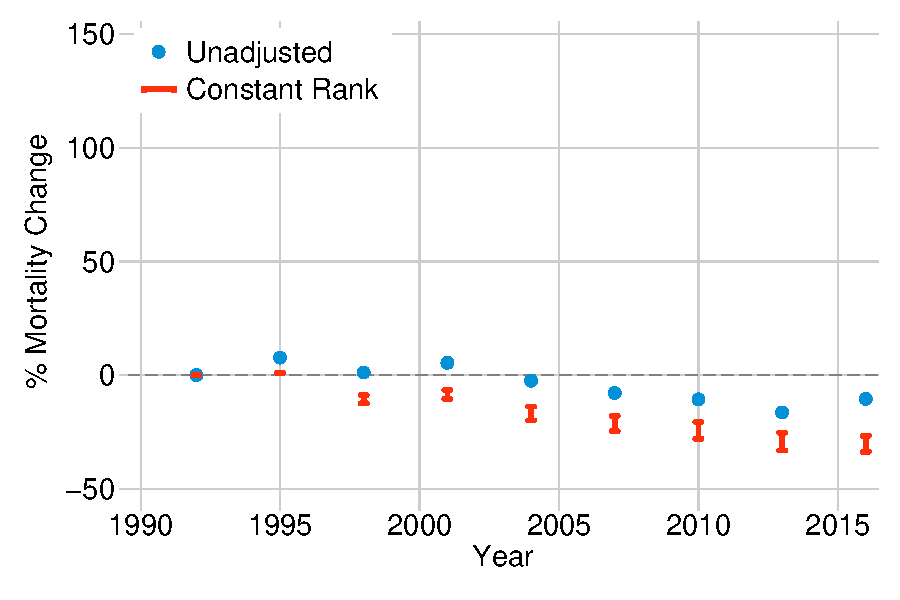
\includegraphics[scale=0.6]{\mortalitypath/naive-2-women-50-t-2} \\

      \multicolumn{2}{c}{\textul{Black Men}} \\
      Dropouts vs. p0--p17 & High School vs. p17--p52 \\
      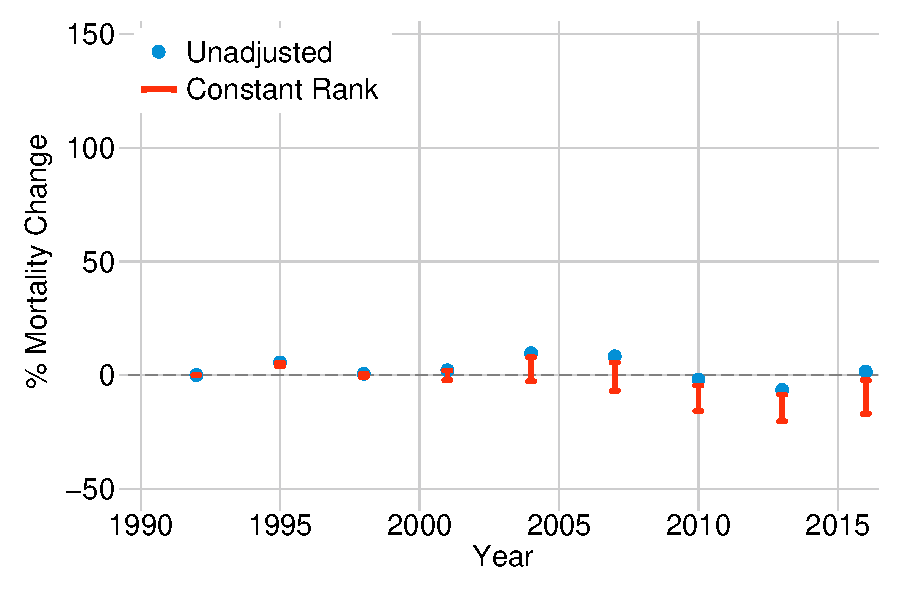
\includegraphics[scale=0.6]{\mortalitypath/naive-2-men-50-t-1} &
      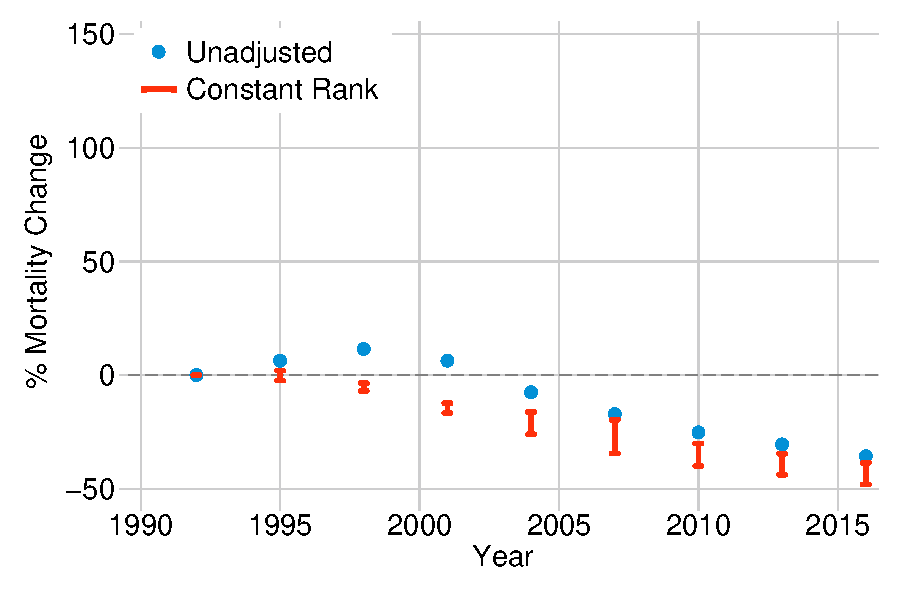
\includegraphics[scale=0.6]{\mortalitypath/naive-2-men-50-t-2} \\

    \end{tabular}
    
  \end{center}
  \footnotesize{Note: ``White'' refers to non-Hispanic white and ``Black'' to non-Hispanic black. The line segments in the graph show bounds on age-adjusted mortality change from 1992--1994 to 2016--2018 for 50-year-olds, separately by race and gender. The four education groups represent education percentiles (i) 0--10; (ii) 10--45; (iii) 45--70; and (iv) 70--100.  The points in the graph show naive estimates of mortality rates at fixed education \textit{levels}; the four education levels for the points represent (i) high school dropouts; (ii) high school completers; (iii) some college; and (iv) a B.A. or higher.}
\end{figure}
\end{landscape}


% \floatbarrier

\newpage 
\clearpage 
\section{Appendix: Data Construction}
\label{sec:app_data}
\spacing{1.5} 
\normalsize This section provides additional details on data construction.  The
All Cause Mortality file provided by the National Center for Health
Statistics reports the number of deaths, by age, race, gender,
education and state.

\textbf{Mortality data.} Beginning in 2003, a substantial share of states only report
educations in coarse bins. The bins are: 
\begin{itemize}
\item 8th grade or less
\item 9th - 12th grade, no diploma
\item High school graduate or GED 
\item Some college, but no degree
\item Associate degree
\item Bachelor's degree
\item Master's degree
\item Doctorate or professional degree
\item Unknown 
\end{itemize}

To reduce noise, we slightly coarsen the bins. We put the small share of people
people with an 8th grade or less into the HS Dropouts group. We aggregate HS dropouts and
middle-school dropouts due to concerns about statistical precision.

We aggregate some college and Associate degrees into the Some College
group; it is not clear which group would have
higher rank or socioeconomic status on average. To reduce noise, we aggregate
Bachelor's, Master's, and Doctorate/professional degrees. These
aggregation choices are unlikely to affect our estimates of mortality
at the bottom of the distribution. 

We exclude deaths of foreign residents. 

\textbf{Missing education.} Georgia, Oklahoma, Rhode
Island, and South Carolina do not consistently report education data
linked to the death certificates. Because
their entry and exit from the data could bias mortality trends, we
drop mortality records and population totals for these states. The
mortality rates we report are thus mortality rates for the remaining states. 

The remaining mortality records occasionally report missing
education. In each age-gender-race-year category, we obtain the
proportion of death records with non-missing educations belonging to
each education group. We assign an education group to mortality
records where education is missing, assuming that the missing
distribution is the same as the non-missing distribution. For example,
if 25\% of mortality records with non-missing education in a
given cell have a high school degree only, we assign 25\% of the
mortality records with missing education to have a high school
degree. This practice is standard; see Case and Deaton
(\citeyear{Case2015,Case2017}).

Missing data cannot account for the large mortality changes
described in the body of the paper. After dropping the four states, 2.90\% of
white and 4.34\% of black mortality records are missing
education (across all years). Roughly 20\% of missing deaths among
whites (and 25\% among blacks) are assigned to high school
dropouts; even in the extreme case where \textit{all} of these
assignments were incorrect, it would erroneously assign only about 0.6\%
of white and 1\% of black deaths to the bottom education bin, thus creating very
little bias.\footnote{By 2000 and after, the share of missing data falls by
  about a third. Thus, the trends over the past 18 years are even less subject to this
  concern.} 

\textbf{CPS.} Following \cite{Case2017}, we use the March
CPS extracts prepared by the Center for Economic and Policy
Research. 

\textbf{Harmonizing educations.} A standard issue when harmonizing
educational attainment data across several datasets is the treatment
of people who drop out of high school in 12th grade. \citet{Jaeger1997}
recommends treating 12th grade dropouts as people who complete
high school, since in earlier datasets, people who complete part of
12th grade were typically treated as people who completed
high-school. Therefore, following \citet{Jaeger1997}'s advice, in the CPS and ACS data which
have fine information about educational attainment, we code people who
drop out of high school in 12th grade as completing high
  school.\footnote{This is automatically implemented in CEPR's public-use CPS
    data. When we augment the CPS data with the ACS data, we recode
    CEPR's ACS education variable so it is consistent with the CPS
    data.}

Early mortality data reports years of
school completed. Beginning in 2003, a share of states began reporting
education in \textit{categories}, where one of the categories is
9th--12th grade, no diploma. By 2018, all deaths are coded using the
2003 categories. It is not possible to disaggregate the
data further. Before 2003, the data only include years of high school
(e.g., 1 year of high school or 4 years of high school). For the data
coded using the pre-2003 categories, we consider dropouts to be people
who attained less than 4 years of high school.

We acknowledge a concern that beginning in 2003, we include people who
attained some 12th grade education as dropouts. We emphasize that, due to
the death certificate aggregation, there is no
other way to harmonize the mortality data over time. However, this data
limiation is unlikely to play a large role in our results. For example, in the 2018
ACS, there are approximately 5 million people who have 12th grade, no
diploma. By contrast, there are 86 million people who do not attain a
high-school degree (and have no 12th grade education at all) and 70
million people who attain a high-school diploma. As a result, the
share of people who receive some 12th grade education but no degree
represents 7\% or less of either group.

\textbf{Moving averages.} Because we use
small population cells (e.g., white high-school dropouts ages 30--34),
to address noise, we use the moving 5-year average for the total population
denominator when 5 years of data are available. In 1993 and 2017, we
use the moving 3-year average (1992--1994 and 2016--2018,
respectively). In 1992 and 2018, we use the predicted values from a
regression of population totals on the adjacent years (1992--1994 and
2016--2018, respectively). 
\begin{itemize}
\item We do not use the 1990 or 1991 CPS data because
the education question changed in 1992, so the estimates of the
dropouts population is discontinuous in 1991. 
\item We do not use the 2019 or 2020 CPS because these extracts are
  not yet harmonized by CEPR. 
\end{itemize} 
We pool annual data into 3-year bins to focus on long-term trends and minimize spurious year-on-year variation in results; e.g. for 1992--94, we use average CPS population in each group and the average number of deaths in each group.

\textbf{Institutionalized populations.} The CPS does not survey
institutionalized populations, e.g. people living in prisons or
hospitals, but deaths in institutions are counted in the mortality
records. To obtain accurate mortality rates, we generate
institutionalized populations in each year as follows:
\begin{enumerate} 
\item We obtain counts of the institutionalized population by age,
  education, gender, race, and year in the 1990 and 2000 
  U.S. Census \citep{ipums} and 2006--2018 American Communities Survey \citep{acs}.
\item For years between Censuses (1991--1999) or between the Census
  and American Communities Survey (2001--2005), we impute the
  number of institutionalized people in each
  age-education-gender-race-year by generating a linear prediction of the
  population between nearest surveys. We use the 2006 ACS because it
  has more accurate counts of the institutionalized populations. For example, if there were 1,000
  institutionalized white women aged 50--54 with a high school degree in
  the 1990 Census and 1,200 in the 2000 Census, we would impute 1,100 in
  1995 (where there is no Census available). 
\item We add institutionalized populations to our count of the
  non-institutionalized populations from the CPS. We compute mortality
  rates as the number of deaths divided by the total population. 
\end{enumerate}

In the ages in our sample, this procedure gives that the share of the
white (black) male institutionalized population was
1.3\% (6.2\%) in 2018. The share of the white (black) female
institutionalized population was 0.5\% (0.7\%). In order for errors
from this imputation process to substantially bias
mortality estimates, the institutionalized population would need to
fluctuate non-linearly in the imputed years. Incarceration rates do rise
substantially in the 1990s, but the change is close to linear over
time, suggesting that the imputation is a good approximation.

The 2018 CPS does not include people living in college dormitories. We
do not adjust for this because we only consider the population older
than age 25. 

\textbf{Cause of deaths.} We partition all deaths into five groups:
cancer, heart disease, deaths of despair, injuries, and other
diseases. We construct these groups by using codes from the
International Statistical Classification of Diseases and Related
Health Problems. NCHS reports ICD-9 codes for 1992--1998 and ICD-10
codes for 1999--2018. We list below the codes pertaining to each cause
of death. For consistency, we follow the data appendix and public code
from \citet{Case2017} to define deaths from cancer,
heart disease, and deaths of despair.

\begin{itemize}
\item Cancer. ICD-9: 140--208; ICD-10: C (all). 
\item Heart Disease. ICD-9: 390-429; ICD-10: I0--I9, I11, I13,
  I20--I51. 
\item Deaths of Despair. ICD-9: 571, 850--860, 950--959, 980; ICD-10:
  K70, K73, K74, X40--45, Y10--15, Y45, Y47, Y49, Y87.0. 
\item Injuries. ICD-9: 800-999 \& not a death of despair;
  ICD-10: V, W, X, Y \& not a death of despair. 
\item Other Diseases. All deaths not otherwise classified. 
\end{itemize}

Table~\ref{tab:icd_causes} reports the share of deaths among
25--69-year-olds in 2018, ordered by importance. We report the
categories used in the paper, and then disaggregate remaining deaths
according to major ICD-10 categories.
 
% \floatbarrier

\newpage 
\clearpage
\section{Appendix: Methods}
\renewcommand{\thefigure}{C\arabic{figure}}
\setcounter{figure}{0}
\renewcommand{\thetable}{C\arabic{table}}
\setcounter{table}{0}

\subsection{Analytical Proof of NRA Bounds}
\label{sec:app_proofs}
\normalsize \subsubsection{Proof of Proposition \ref{eq:cef_bound}}
Formalizing the set-up from the text, let $y \sim F$, where
$F$ has support $[\underline{y},\overline{y}]$. Put $r_0 =
\underline{y}$ and $r_{K+1} = \overline{y}$. In our benchmark case 
where $y$ denotes survival rates, $F$ has support $[0,1]$. For simplicity we impose $F$ has
finite support in all proofs below. The arguments are identical if $F$
has infinite support except in the top or bottom bin, where the
bounds must be adjusted slightly.\footnote{We focus on finite-support $F$ to lighten
  notation. In practice for
  the analyst, almost every distribution can be restricted with only
  slight loss of generality to have finite support. For instance, if one
  studies the CEF of wages given education, $\overline{y}$ can be set
  to an implausibly high value.}

\textit{Part 1: Find} $x_k^*$. First define $\mathcal{V}_k$ as the
set of weakly increasing CEFs which meet the bin mean. Put
otherwise, let $\mathcal{V}_k$ be the set of weakly increasing $v: [x_k,x_{k+1}] \to \mathbb{R}$
satisfying $$r_k = 
\frac{1}{x_{k+1} - x_k} \int_{x_k}^{x_{k+1}} v(x) dx.$$ 
Now choose $z \in \mathcal{V}_k$ such that 
$$
z(x) = \begin{cases} 
r_{k-1}, & x_k \leq x < j \\
r_{k+1}, & j \leq x \leq x_{k+1}.
\end{cases} 
$$

Note that $z$ and $j$
both exist and are unique (it suffices to show that just $j$ exists
and is unique, as then $z$ must be also). We can solve for $j$ by
noting that $z$ lies in $\mathcal{V}_k$, so it must meet the bin mean. Hence, by
evaluating the integrals, $j$ must satisfy: 
\begin{align*}
r_k &= \frac{1}{x_{k+1} - x_k} \int_{x_k}^{x_{k+1}} z(x) dx \\
&= \frac{1}{x_{k+1} - x_k} \left(\int_{x_k}^{j} r_{k-1} dx
+  \int_{j}^{x_{k+1}} r_{k+1} dx \right) \\ 
&= \frac{1}{x_{k+1} - x_k} \left( \left(j - x_k\right)
r_{k-1} + \left(x_{k+1} - j\right) r_{k+1} \right). 
\end{align*}
Note that these expressions invoke assumption U, as the integration
of $z(x)$ does not require any adjustment for the density on the $x$ axis. For a
more general proof with an arbitrary distribution of $x$, see the
following section. 

With some algebraic manipulations, we obtain that $j =
x_k^*$.

\textit{Part 2: Prove the bounds.} 
In the next step, we show that $x_k^*$ is the smallest point at which no
$v \in \mathcal{V}_k$ can be $r_{k-1}$, which means that there must be some
larger lower bound on $E(y | x)$ for $x \geq x_k^*$. In other words, we prove
that $$x_k^* = \sup \Big\{x \vert \text{ there exists } v \in \mathcal{V}_k \text{
such that
} v(x) = r_{k-1}. \Big\}.$$ We must show that $x_k^*$ is an upper bound
and that it is the least upper bound. 

First, $x_k^*$ is an upper bound. Suppose that there exists $j' > x_k^*$ such
that for some $w \in \mathcal{V}_k$, $w(j') = r_{k-1}$. Observe that by
monotonicity and the bounds from \citet{Manski2002}, $w(x) =
r_{k+1}$ for $x \leq j'$; in other words, if $w(j')$ is the mean of
the mean of the prior bin, it can be no lower or higher than the mean
of the prior bin up to point $j'$. But since $j' > j$, this means that 
$$ \int_{x_k}^{j'} w(x)dx < \int_{x_k}^{j'} z(x) dx,$$ since $z(x) >
w(x)$ for all $h \in (j,j')$. But recall that both $z$ and $w$ lie in
$\mathcal{V}_k$ and must therefore meet the bin mean; i.e., 
$$ \int_{x_k}^{x_{k+1}} w(x)dx = \int_{x_k}^{x_{k+1}}
z(x)dx.$$ 
But then $$\int_{j'}^{x_{k+1}} w(x)dx > \int_{j'}^{x_{k+1}} z(x)
dx.$$ That is impossible by the bounds
from \citet{Manski2002}, since $w(x)$ cannot exceed
$r_{k+1}$, which is precisely the value of $z(x)$ for $x \geq j$. 

Second, $j$ is the least upper bound. Fix $j' < j$. From the definition of $z$, we
have shown that for some $h \in (j',j)$, $z(h) = r_{k-1}$ (and $z \in
\mathcal{V}_k$). So any point $j'$ less than $j$ would not be a lower bound on the
set --- there is a point $h$ larger than $j'$ such that $z(h) =
r_{k-1}$. 

Hence, for all $x < x_k^*$, there exists a function $v \in \mathcal{V}_k$ such
that $v(x) = r_{k-1}$; the lower bound on $E(y | x)$ for $x < x_k^*$
is no greater than $r_{k-1}$. By choosing $z'$ with 
$$ 
z'(x) = \begin{cases} 
r_{k-1}, & x_k \leq x \leq j \\
r_{k+1}, & j < x \leq x_{k+1}, 
\end{cases} 
$$ 
it is also clear that at $x_k^*$, the lower bound is no larger 
than $r_{k-1}$ (and this holds in the proposition itself, substituting in
$x_k^*$ into the lower bound in the second equation).

Now, fix $x' \in (x_k^*, x_{k+1}]$. Since $x_k^*$ is the supremum, there
is no function $v \in \mathcal{V}_k$ such that $v(x') = r_{k-1}$. Thus for
$x' > x_k^*$, we seek a sharp lower bound larger than $r_{k-1}$. Write this lower bound as
$$Y_{x'}^{min} = \min \Big\{ v(x') \text{ for all  } v \in \mathcal{V}_k \Big\},$$
where $Y_{x'}^{min}$ is the smallest value attained by any function $v \in \mathcal{V}_k$ at the point
$x'$. 

We find this $Y_{x'}^{min}$ by choosing the function which maximizes
every point after $x'$, by attaining the value of the
subsequent bin. The function which minimizes $v(x')$ must be a
horizontal line up to this point. 

Pick $\tilde{z} \in \mathcal{V}_k$ such that 
$$ 
\tilde{z}(x) = \begin{cases}
\underline{Y}, &x_k \leq x' \\
r_{k+1}, &x' < x_{k+1} 
\end{cases}. 
$$
By integrating $\tilde{z}(x)$, we claim that $\underline{Y}$ satisfies the following: 
$$ \frac{1}{x_{k+1} - x_k} \left( \left(x' - x_k\right) \underline{Y} + \left(x_{k+1} -
x'\right) r_{k+1}\right) = r_k .$$ As a result, $\underline{Y}$ from this expression exists and is unique,
because we can solve the equation. Note that this integration step
also requires that the distribution of $x$ be uniform, and we
generalize this argument in the following section. 

By similar reasoning as above, there
is no $Y' < \underline{Y}$ such that there exists $w \in \mathcal{V}_k$ with 
$w(x') = Y'$. Otherwise there must be some point $x
> x'$ such that $w(x') > r_{k+1}$ in order that $w$ matches the bin
means and lies in $\mathcal{V}_k$; the expression
for $\underline{Y}$ above maximizes every point after $x'$, leaving no
additional room to further depress $\underline{Y}$. 

Formally, suppose there exists $w \in \mathcal{V}_k$ such that $w(x') =
Y' < \underline{Y}$. Then $w(x') < \tilde{z}(x')$ for all $x < x'$, since $w$ is
monotonic. As a result, $$\int_{x_k}^{x'}\tilde{z}(x)dx
>  \int_{x_k}^{x'}w(x)dx.$$ But recall that 
$$\int_{x_k}^{x_{k+1}} w(x) dx = \int_{x_k}^{x_{k+1}} \tilde{z}(x) dx,$$ so 
$$\int_{x'}^{x_{k+1}} w(x) dx > \int_{x'}^{x_{k+1}} \tilde{z}(x) dx. $$ This is
impossible, since $\tilde{z}(x) = r_{k+1}$ for all $x > x'$, and
by \citet{Manski2002}, $w(x) \leq r_{k+1}$ for all $w \in \mathcal{V}_k$. Hence there
is no such $w \in \mathcal{V}_k$, and therefore $\underline{Y}$ is smallest possible
value at $x'$, i.e. $\underline{Y} = Y_{x'}^{min}$.

By algebraic manipulations, the expression for $\underline{Y} = Y_{x}^{min}$ reduces
to $$Y_{x}^{min} = \frac{ \left(x_{k+1} - x_k\right) r_k  - (x_{k+1}
- x) r_{k+1}}{x - x_k}, \ x \geq x_k^*.$$  

The proof for the upper bounds uses the same structure as the proof of the lower bounds.

Finally, the body of this proof gives sharpness of the bounds. For we
have introduced a CEF $v \in \mathcal{V}_k$ that obtains the value of the upper and lower
bound for any point $x \in [x_k,x_{k+1}]$. For any value $y$ within the
bounds, one can generate a CEF $v \in \mathcal{V}_k$ such that $v(x) =
y$. \qed

\vspace{1em}

\vspace{2em}

\subsubsection{Analytical Bounds when Uniformity Does Not Hold} 
Suppose we relax
assumption $U$. We continue to impose for notational simplicity that $x$ is drawn
from a continuous distribution, though similar arguments apply to discrete
$x$. We characterize $x$ by some known probability
density function, which we assume is integrable in every bin
$k$. Then we derive the following bounds. 

\begin{proposition} 
\label{eq:bound_arb_distrib}
Let $x$ be in bin $k$. For simplicity we work with continuous
distributions of $x$. Let $f_k(x)$ be the probability density function
of $x$ in bin $k$. Under assumptions M, I, MI \citep{Manski2002}, and
without additional information, the
following bounds on $E(y \vert x)$ are sharp:
$$
\begin{cases}                                                                                                                          
r_{k-1} \leq E(y \vert x) \leq \frac{r_k - r_{k-1} \int_{x_{k}}^x
  f_k(s)ds}{\int_x^{x_{k+1}}f_k(s)ds}, & x < x_k^*      \\           
\frac{r_k - r_{k+1}\int_x^{x_{k+1}} f_k(s)ds }{\int_{x_k}^x f_k(s)ds}  \leq E(y \vert x)  \leq                                                                         
r_{k+1} , & x \geq x_k^*                                                                                                             
\end{cases}
$$
where $x_k^*$ satisfies: 
$$r_k = r_{k-1} \int_{x_k}^{x_k^*} f_k(s) ds + r_{k+1}
\int_{x_k^*}^{x_{k+1}} f_k(s) ds.$$ 
\end{proposition} 

The proof follows the same argument as in Proposition
\ref{eq:cef_bound}. With an arbitrary distribution, $\mathcal{V}_k$ now
constitutes the functions $v: [x_k,x_{k+1}] \to \mathbb{R}$ which satisfy: 
$$ \int_{x_k}^{x_{k+1}} v(s)f_k(s) ds = r_k.$$ 

As before, choose $z \in \mathcal{V}_k$ such that 
$$
z(x) = \begin{cases} 
r_{k-1}, & x_k \leq x < j \\
r_{k+1}, & j \leq x \leq x_{k+1}. 
\end{cases}
$$

Because the distribution of $x$ is no longer uniform, $j$ must now satisfy 
\begin{align*}
r_k &= \int_{x_k}^{x_{k+1}} z(s)f_k(s) ds \\ 
&= r_{k-1} \int_{x_k}^j f_k(s)ds + r_{k+1} \int_{j}^{x_{k+1}}
f_k(s)ds. 
\end{align*} 
This implies that $j = x_k^*$, precisely. 

The rest of the arguments follow identically, except we now claim that
for $x > x_k^*$, 
$\underline{Y} = Y_{x}^{min}$ satisfies the following: 
$$ r_k = \int_{x_k}^{x} Y_{x}^{min} f_k(s)ds + \int_{x}^{x_{k+1}}
r_{k+1} f_k(s)ds.$$ 

By algebraic manipulations, we obtain: 
$$ Y_{x}^{min}= \frac{r_k - r_{k+1} \int_{x}^{x_{k+1}}
f_k(s)ds}{\int_{x_k}^{x}  f_k(s)ds}$$ and the proof of the lower
bounds is complete. As before, the proof for upper bounds follows from identical logic. \qed 

\subsubsection{Bounds on $\mu_a^b$}
Define $$  \mu_a^{b} = \frac{1}{b - a} \int_a^{b} E(y | x) di. $$ Let
$Y_x^{min}$ and $Y_x^{max}$ be the lower and upper bounds respectively
on $E(y | x)$ given by Proposition \ref{eq:cef_bound}. 
We seek to bound $\mu_a^b$ when $x$ is observed only in discrete intervals. 

\begin{proposition}
  \label{eq:mu} 
  Let $b \in [x_k, x_{k+1}]$ and $a \in [x_h, x_{h+1}]$ with $a<b$. Let
  assumptions M, I, MI \citep{Manski2002} and U hold. Then, if there is no
  additional information available, the
  following bounds are sharp: 
  \label{eq:bound_mu} 
$$ 
  \begin{cases} 
     Y_b^{min} \leq \mu_a^b \leq Y_a^{max}, & h = k \\
    \frac{r_h (x_k - a) + Y_b^{min}(b - x_k)}{b-a} \leq
    \mu_a^b \leq \frac{Y_a^{max} (x_k - a) + r_k
      (b-x_k)}{b-a}, & h +
    1 = k \\
    \frac{r_h (x_{h+1} - a) + \sum_{\lambda = h+1}^{k-1} r_{\lambda}
      (x_{\lambda+1} - x_{\lambda}) + Y_b^{min}(b - x_k)}{b-a} \leq
    \mu_a^b 
    %% \ \ \ \ \ \ \ \ \ \ \ \ %%
    \leq \frac{Y_a^{max} (x_{h+1} - a) + \sum_{\lambda = h+1}^{k-1} r_{\lambda}
      (x_{\lambda+1} - x_{\lambda}) + r_k (b-x_k)}{b-a}, & h +
    1 < k. 
  \end{cases} 
$$ 
\end{proposition} 

The order of the proof is as follows. If $a$ and $b$ lie in the same
bin, then $\mu_a^b$ is maximized only if the CEF is minimized prior to
$a$. As in the proof of proposition \ref{eq:cef_bound}, that occurs when
the CEF is a horizontal line at $Y_x^{min}$ up to $a$, and a
horizontal line $Y_x^{max}$ at and after $a$. If $a$ and $b$ lie in separate bins, the
value of the integral in bins that are contained between $a$ and $b$ is determined by
the observed bin means. The portions of the integral that are not
determined are maximized by a similar logic, since they both lie
within bins. We prove the bounds for
maximizing $\mu_a^b$, but the proof is symmetric
for minimizing $\mu_a^b$. 

\textit{Part 1: Prove the bounds if $a$ and $b$ lie in the same bin.} We
seek to maximize $\mu_a^b$ when $a, b \in [x_k,x_{k+1}]$. This
requires finding a candidate CEF $v \in \mathcal{V}_k$ which maximizes $\int_a^b
v(x) dx$. Observe that the function
$v(x)$ defined as $$ v(x) = \begin{cases}
Y_a^{min}, &x_k \leq x < a \\ 
Y_a^{max}, &a \leq x \leq x_{k+1} 
\end{cases}
$$ 
has the property that $v \in \mathcal{V}_k$. For if $a \geq x_k^*$, $v = \tilde{z}$
from the second part of the proof of
proposition \ref{eq:cef_bound}. If $a < x_k^*$, the CEF in $\mathcal{V}_k$ which
yields $Y_a^{max}$ is precisely $v$ (by a similar argument which delivers the upper bounds in
proposition \ref{eq:cef_bound}). 

This CEF maximizes $\mu_a^b$, because
there is no $w \in \mathcal{V}_k$ such that $$\frac{1}{b-a} \int_{a}^{b}
w(x) dx > \frac{1}{b-a}
\int_{a}^{b} v(x)dx.$$ Note that for any $w \in \mathcal{V}_k$, $\frac{1}{x_{k+1} - x_k} \int_{x_k}^{x_{k+1}} w(x)dx =
\frac{1}{x_{k+1} - x_k} \int_{x_k}^{x_{k+1}} v(x)dx = r_k$. Hence in
order that $\int_{a}^{b} w(x)dx > \int_{a}^{b} v(x)dx$, there are two
options. The first option is that $$ \int_{x_k}^{a}
w(x)dx < \int_{x_k}^{a} v(x)dx.$$ That is impossible, since there is
no room to depress $w$ given the value of $v$ after $a$. If $a < x_k^*$, then it is
clear that there is no $w$ giving a larger $\mu_a^b$, since
$r_{k-1} \leq w(x)$ for $x_{k-1} \leq x \leq a$, so $w$ is bounded below by $v$. If $a \geq x_k^*$, then $v(x) = r_{k+1}$ for all $a \leq x \leq
x_{k+1}$. That would leave no room to depress $w$ further; if $ \int_{x_k}^{a}
w(x)dx < \int_{x_k}^{a} v(x)dx$, then $\int_{a}^{x_{k+1}} w(x) dx
> \int_{a}^{x_{k+1}} v(x) dx $, which cannot be the case if $v =
r_{k+1}$, by the bounds given in \citet{Manski2002}. 

The second option is that $$ \int_{b}^{x_k}
w(x)dx < \int_{b}^{x_k}
v(x)dx .$$ This is impossible due to monotonicity. For if $ \int_{a}^{b}
w(x)dx > \int_{a}^{b}
v(x)dx$, then there must be some point $x' \in [a,b)$ such that $w(x')
> v(x')$. By monotonicity, $w(x) > v(x)$ for all $x \in [x',x_{k+1}]$
since $v(x) =Y_a^{max}$ in that interval. As a result,  $$ \int_{b}^{x_k}
w(x)dx > \int_{b}^{x_k}
v(x)dx,$$ since $b \in (x',x_{k+1})$. (If $b = x_{k+1}$, then only the
first option would allow $w$ to maximize the desired $\mu_a^b$.) 

Therefore, there is no such $w$, and $v$ indeed maximizes the desired integral. Integrating $v$ from
$a$ to $b$, we obtain that the upper bound on $\mu_a^b$ is
$\frac{1}{b-a} \int_a^b Y_a^{max} dx = Y_a^{max}$. Note that there may
be many functions which maximize the integral; we only needed to show
that $v$ is one of them. 

To prove the lower bound, use an analogous argument. 

\textit{Part 2: Prove the bounds if $a$ and $b$ do not lie in the same
bin.} We now generalize the set up and permit $a,b \in [0,100]$. Let
  $\mathcal{V}$ be the set of weakly increasing functions such that $\frac{1}{x_{k+1} -
  x_k} \int_{x_k}^{x_{k+1}}
v(x) dx = r_k$ for all $k \leq K$. In other words, $\mathcal{V}$ is the set of
  functions which match the means of every bin. Now observe that for all $v \in \mathcal{V}$, 
\begin{align*}
\mu_a^b &= \frac{1}{b-a}\int_a^b v(x) dx \\ 
&= \frac{1}{b-a} \left(
\int_a^{x_{h+1}} v(x)dx + \int_{x_{h+1}}^{x_k} v(x)dx +
\int_{x_k}^{b} v(x) dx \right), 
\end{align*} 
by a simple expansion of the integral. 

But for all $v \in \mathcal{V}$, $$\int_{x_{h+1}}^{x_k} v(x)dx = \sum_{\lambda =
  h+1}^{k-1} r_{\lambda}
    (x_{\lambda+1} - x_{\lambda})$$ if $h + 1 <k$
and $$\int_{x_{h+1}}^{x_k} v(x)dx = 0$$ if $h + 1 = k$. For in
  bins completely contained inside $[a,b]$, there is no room for any
  function in $\mathcal{V}$ to vary; they all must meet the bin means. 

We proceed to prove the upper bound. We split this into two portions:
we wish to maximize $\int_a^{x_{h+1}}v(x)dx $ and we also wish to maximize $\int_{x_k}^b v(x)dx $. The values of
these objects are not codependent. But observe that the CEFs $v \in
\mathcal{V}_k$ which yield upper bounds on these integrals are the very same functions which yield upper bounds on
$\mu_a^{x_{h+1}} $ and $\mu_{x_k}^b$, since $\mu_s^t
= \frac{1}{t-s} \int_s^t v(x) dx$ for any $s$ and $t$. Also notice
that $a$ and $x_{h+1}$ both lie in bin $h$, while $b$ and $x_k$ both
lie in bin $k$, so we can make use of 
the first portion of this proof. 

In part 1, we showed that the function $v \in \mathcal{V}$, 
$v:[x_h,x_{h+1}] \to \mathbb{R}$, which maximizes $\mu_a^{x_{h+1}}
$ is
$$ v(x) = \begin{cases}
Y_a^{min}, & x_{h} \leq x < a \\
Y_a^{max}, & a \leq x \leq x_{h+1}. 
\end{cases}
$$ 
As a result $$\underset{v \in \mathcal{V}}{\max}\Bigg\{ \int_a^{x_{h+1}} v(x) dx \Bigg\} = \int_a^{x_{h+1}} Y_a^{max} dx = Y_a^{max} (x_{h+1} -a).$$

Similarly, observe that $x_k$ and $b$ lie in the same bin, so the function
$v:[x_k,x_{k+1}] \to \mathbb{R}$, with $v \in \mathcal{V}$  which maximizes $\int_{x_k}^b v(x)dx$ must be of the form 
$$ v(x) = \begin{cases}
Y_{x_k}^{min}, & x_{k} \leq x < a \\
Y_{x_k}^{max}, & b \leq x \leq x_{k+1}. 
\end{cases}
$$ 

With identical logic, 
$$\underset{v \in \mathcal{V}}{\max}\Bigg\{ \int_{x_k}^{b} v(x) dx \Bigg\}
= \int_{x_k}^{b} Y_{x_k}^{max} dx = Y_{x_k}^{max} (b -x_k).$$
And by proposition \ref{eq:cef_bound}, $x_k \leq x_k^*$ so $Y_{x_k}^{max} =
r_{k}$. (Note that if $x_k = x_k^*$, substituting $x_k^*$ into the second
expression of proposition \ref{eq:cef_bound} still yields that
$Y_{x_k}^{max} = r_k$.) 

Now we put all these portions together. First let $h + 1 = k$. Then
$\int_{x_{h+1}}^{x_k} v(x) dx = 0$, so 
we maximize $\mu_a^b$ by
$$\frac{1}{b-a} \left( Y_a^{max} (x_{h+1} -a) + r_k (b
-x_k) \right). $$ Similarly, if $h +1 < k$ and there are entire bins completely
contained in $[a,b]$, then we maximize $\mu_a^b$ by 
$$\frac{1}{b-a} \left( Y_a^{max} (x_{h+1} -a) + \sum_{\lambda =
  h+1}^{k-1} r_{\lambda}
    (x_{\lambda+1} - x_{\lambda}) + r_k  (b -x_k) 
\right). $$ 

The lower bound is proved analogously. Sharpness is immediate, since
we have shown that the CEF which delivers the endpoints of the
bounds lies in $\mathcal{V}$. As a result, there is a function delivering any intermediate
value for the bounds. \qed 

\vspace{1em}
 

\subsection{Numerical Calculation of NRA Bounds with Arbitrary Structural Assumptions} 
\label{sec:app_numerical} 
\normalsize This section describes the numerical optimization approach for
calculating bounds on mortality within arbitrary percentiles of the
education distribution. To calculate bounds, we discretize the mortality-education relationship and solve a numerical optimization problem that obtains the highest and lowest possible values of expected mortality at any given point, that are consistent with matching the empirical data points and meeting a set of structural constraints on the functional form of the CEF. We first formalize the computational procedure and then describe its numerical implementation.

\subsubsection{Conceptual Approach: Functions of the CEF} 
We write the conditional expectation function in the form
$Y(x) = s(x,\gamma)$, where $\gamma$ is a finite-dimensional vector
that lies in parameter space $G$ and serves to parameterize the CEF
through the function $s$. For example, we could estimate the
parameters of a linear approximation to the CEF by defining
$s(x,\gamma)=\gamma_0+\gamma_1*x$. We can approximate an arbitrary
nonparametric CEF by defining $\gamma$ as a vector of discrete values
that give the value of the CEF in each of $N$ partitions; we take this
approach in our numerical optimizations, setting $N$ to
100.\footnote{For example, $s(x,\gamma_{50})$ would represent $E(y|x
  \in [49,50])$.} Any statistic $m$ that is a single-valued function
of the CEF, such as the average value of the CEF in an interval
$(\mu_a^b)$, or the slope of the best fit line to the CEF, can be
defined as $m(\gamma)=M(s(x,\gamma))$.

Let $f(x)$ represent the probability distribution of $x$. Define $\Gamma$ as the set of parameterizations of the CEF that obey monotonicity and minimize mean squared error with respect to the observed interval data:
\begin{align}
  \label{eq:opt1}
  \Gamma = \underset{g \in G}{\text{argmin}} \sum_{k=1}^K \Bigg\{
  \int_{x_k}^{x_{k+1}} f(x) dx \left( \left(
  \frac{1}{\int_{x_k}^{x_{k+1}} f(x)dx } \int_{x_k}^{x_{k+1}} s(x,g)
  f(x) dx \right) - \overline{r}_k \right)^2 \Bigg\} \\ \nonumber
  \text{such that} \\ \tag{Monotonicity} s(x,g) \text{ is weakly
    increasing in } x.
\end{align}
\noindent Decomposing this expression, $\frac{1}{\int_{x_k}^{x_{k+1}}
  f(x)dx } \int_{x_k}^{x_{k+1}} s(x,g) f(x) dx$ is the mean value of
$s(x,g)$ in bin $k$, and $\int_{x_k}^{x_{k+1}} f(x) dx$ is the mass in
bin $k$. The minimand is thus a bin-weighted MSE.\footnote{While we
  choose to use a weighted mean squared error penalty, in principle
  $\Gamma$ could use other penalties.} Recall that for the rank
distribution, $x_1=0$ and $x_{K+1}=100$. We can easily add additional
structural constraints on $s(x,\gamma)$ to Equation \ref{eq:opt1} (e.g., the curvature
constraint below) or remove the monotonicity constraint. 

The bounds on $m(\gamma)$ are therefore:

\begin{equation}
  \begin{aligned}
    \label{eq:m_bounds}
    m^{min} &= \inf\{m(\gamma) \ \vert \ \gamma \in \Gamma \} \\ m^{max} &= \sup\{m(\gamma) \ \vert \ \gamma \in \Gamma \}.
  \end{aligned}
\end{equation}

For example, bounds on the best linear approximation to the CEF can be defined by the following process. First, consider the set of all CEFs that satisfy monotonicity and minimize mean-squared error with respect to the observed bin means.\footnote{In many cases, and in all of our applications, there will exist many such CEFs that exactly match the observed data and the minimum mean-squared error will be zero.} Next, compute the slope of the best linear approximation to each CEF. The largest and smallest slope constitute $m^{min}$ and $m^{max}$. Note that this definition of the best linear approximator to the CEF corresponds to the \textit{least squares set} defined by \citet{Ponomareva2011}.

The set of CEFs that describe the upper and lower bounds in Proposition~\ref{eq:cef_bound} are step functions with substantial discontinuities. If such functions are implausible descriptions of the data, then the researcher may wish to impose an additional constraint on the curvature of the CEF, which will generate tighter bounds. For example, examination of the mortality-income relationship (which can be estimated at each of 100 income ranks, displayed in Appendix Figure \ref{fig:mort_poly}) suggests no such discontinuities. Alternately, in a context where continuity has a strong theoretical underpinning but monotonicity does not, a curvature constraint can substitute for a monotonicity constraint and in many cases deliver useful bounds.

We consider a curvature restriction with the following structure:
\begin{align}
  \label{eq:c_bar}
  \tag{Curvature Constraint} \tag{Or alt Curvature} s(x,\gamma) \text{ is twice-differentiable and } \vert s''(x,\gamma) \vert \leq \overline{C}.
\end{align}

\noindent This is analogous to imposing that the first derivative is Lipshitz.\footnote{Let $X, Y$ be metric spaces with metrics $d_X, d_Y$ respectively. The function $f:X \to Y$ is \textit{Lipschitz continuous} if there exists $K \geq 0$ such that for all $x_1,x_2 \in X$,
  $$d_Y(f(x_1),f(x_2)) \leq K d_X(x_1,x_2).$$} Depending on the value
of $\overline{C}$, this constraint may or may not bind. 

The most restrictive curvature constraint, $\overline{C}=0$, is
analogous to the assumption that the CEF is linear. Note that the
default practice in many studies of mortality is to estimate the best
linear approximation to the CEF of mortality given education (e.g.,
\citet{Cutler2011} and \citet{Goldring2016}). A moderate curvature
constraint is therefore a \textit{less} restrictive assumption than
the approach taken in many studies. In practice, we slightly adjust the curvature
constraint condition by generating a ``normalized'' curvature
constraint which imposes that the absolute value of the second
derivative, divided by the mean mortality across all percentiles, does
not exceed a certain $\overline{C}$. The advantage of this approach is
that it more readily permits using a conservative value of $\overline{C}$ across
all groups. We discuss the choice of curvature
restriction below. 

\subsubsection{Computational Approach} 

This section describes a method to numerically solve the constrained optimization problem suggested by Equations~\ref{eq:opt1} and \ref{eq:m_bounds}. 

To make the problem numerically tractable, we solve the discrete problem of identifying the feasible mean value taken by $E(y|x)$ in each of $N$ discrete partitions of $x$. We thus assume $E(y|x) = s(x,\gamma)$, where $\gamma$ is a vector that defines the mean value of the CEF in each of the $N$ partitions. We use $N=100$ in our analysis, corresponding to integer rank bins, but other values may be useful depending on the application. In other words, we will numerically calculate upper and lower bounds on $E(y|x \in [0, 1])$, $E(y|x \in [1, 2])$, $...$, $E(y|x \in [99,100])$.  Given continuity in the latent function, the discretized CEF will be a very close approximation of the continuous CEF; in our applications, increasing the value of $N$ increases computation time but does not change any of our results.

We solve the problem through a two-step process. Define a $N$-valued
vector $\hat{\gamma}$ as a candidate CEF. First, we calculate the
minimum MSE from the constrained optimization problem given by
Equation~\ref{eq:opt1}. Put another way, each set $\Gamma$
  is associated to a minimmum MSE (the value of the objective), which
  we denote $\underbar{MSE}$. We then run a second pair of constrained optimization problems that respectively minimize and maximize the value of $m(\hat{\gamma})$, with the additional constraint that the MSE is equal to the value obtained in the first step, denoted $\underbar{MSE}$. Equation \ref{eq:opt2} shows the second stage setup to calculate the lower bound on $m(\hat{\gamma})$:
\begin{align}
  \label{eq:opt2}
  m^{min} &= \underset{ \hat{\gamma} \in [0,100]^{N} }{ \text{min} } m(\hat{\gamma}) \\
  &\nonumber \text{such that} \\
  \tag{Monotonicity} s(x, \hat{\gamma}) \text{ is weakly increasing in } x \\
  \tag{Curvature} \lvert s''(x, \hat{\gamma}) \rvert &\leq \overline{C} \\
  \tag{MSE Minimization} \sum_{k=1}^K \left[ \frac{\Vert X_k \Vert}{100} \left( \left( \frac{1}{\Vert X_k \Vert} \sum_{x \in X_k} s(x,\hat{\gamma}) \right) - \overline{r}_k \right)^2 \right] &= \underbar{MSE}
\end{align}

\noindent
$X_k$ is the set of discrete values of $x$ between $x_{k}$ and
$x_{k+1}$ and $\Vert X_k \Vert$ is the width of bin
$k$. $\overline{r}_k$ is the observed mortality in education bin $k$,
and \underbar{MSE} is the lowest mean-squared error obtainable out of
the entire set of education-mortality functions, which is typically
zero. The complementary maximization problem obtains the upper bound
on $m(\hat{\gamma})$. Note that this particular setup is specific to
the uniform rank distribution, but setups with other distributions
would be similar. 

The purpose of the two-step process is that it is difficult to
numerically solve for every possible member of $\Gamma$ under
arbitrary constraints. We render the problem tractable by recasting
the problem as a minimization problem of obtaining $\underbar{MSE}$ in
the first step. Then, in the second step, we use $\underbar{MSE}$ as a
constraint. 

Note that setting $m(\gamma) = \gamma_x$ (the $x$\superscript{th} element of $\gamma$) obtains bounds on the value of the CEF at point $x$. Calculating this for all ranks $x$ from 1 to 100 generates analogous bounds to those derived in proposition \ref{eq:cef_bound}, but satisfying the additional curvature constraint. Similarly $m(\gamma) = \frac{1}{b-a} \sum_{x=a}^{b}\gamma_x$ yields bounds on $\mu_a^b$.

The numerical method can easily permit the curvature constraint to vary over the CEF. For example, one might believe that there are discontinuities in the CEF at bin boundaries, due to sheepskin effects \citep{hungerford1987}; high-school graduates, upon receiving a diploma, could experience discretely lower mortality probability due to better labor-market outcomes. In other settings, researchers might impose that the CEF has a large (but finite) curvature in one portion of its domain and be more constrained elsewhere.

\textbf{Calibrating a curvature constraint}.  This subsection explains how we obtain a benchmark for the curvature constraint using data from \citet{Chetty2016b} on mortality rates for U.S. men and women above age 40 from years 2001--2014. We collapse the data to three-year periods and five-year age groups.\footnote{Since the number of years is not divisible by 3, we group years 2001 and 2002.}$^,$\footnote{Because people are ranked within the percentile for their own age, gender, and year, this departs slightly from the ranking procedure we use in the text.} We then use OLS to fit fifth-order polynomials to the mortality-income percentile data we observe. We show two examples of these best-fit functions for 50--54 year old men and women in 2012--2014 (the last year data are available), as well as the range for the normalized second derivative for these groups, in Appendix Figure \ref{fig:mort_poly}. The $\overline{C}$ we use is 50\% larger than the maximum absolute value of the union of these ranges across all such groups we observe.

We construct a $\overline{C}$ that holds for all mortality-income
functions as follows. Using the estimated polynomial fit, we
analytically compute the absolute value of the second derivative of
the best-fit polynomial at every value for every polynomial
function. To generate comparable $\overline{C}$, we construct a normalized $\overline{C}$ that accounts for differences in mortality levels by dividing the absolute value of the second derivative by the mean mortality in that age-year group (across all percentiles). Expressed in these terms (and multiplied by 100), the normalized $\overline{C}$ represents the absolute value of the second derivative as a percent of the mean.

Across all age and years, the largest $\overline{C}$ is approximately 2.0\%. Because polynomial fits can be inaccurate near the tails, we also compute the largest second-derivative (normalized by the mean mortality across all percentiles) within the set of percentiles $[5,95]$. This value is 1.5\%. We choose a conservative curvature constraint of 3\% --- about 50\% larger than the largest normalized $\overline{C}$ observed in the data.

We acknowledge the concern that mortality-income CEFs may exhibit different curvature than mortality-education CEFs. We argue that the mortality-income CEF at least provides a natural benchmark for how curved the CEF might be in the education setting; we are not aware of another continuous conditioning value to calibrate $\overline{C}$. Moreover, we are comforted that our results are robust to relaxing the curvature constraint altogether.

%%%%%%%%%%%%%%%%%%%%%%%%%%%%%%%%
% Mortality rank distributions 
%%%%%%%%%%%%%%%%%%%%%%%%%%%%%%%%
\begin{figure}[H]
  \caption{Fifth-Order Polynomial Approximations to the Empirical Mortality-Income CEF}
  \label{fig:mort_poly}

\begin{center}
  Panel A: 50--54 Year-Old Women in 2012--2014
\end{center}
  \begin{center}
      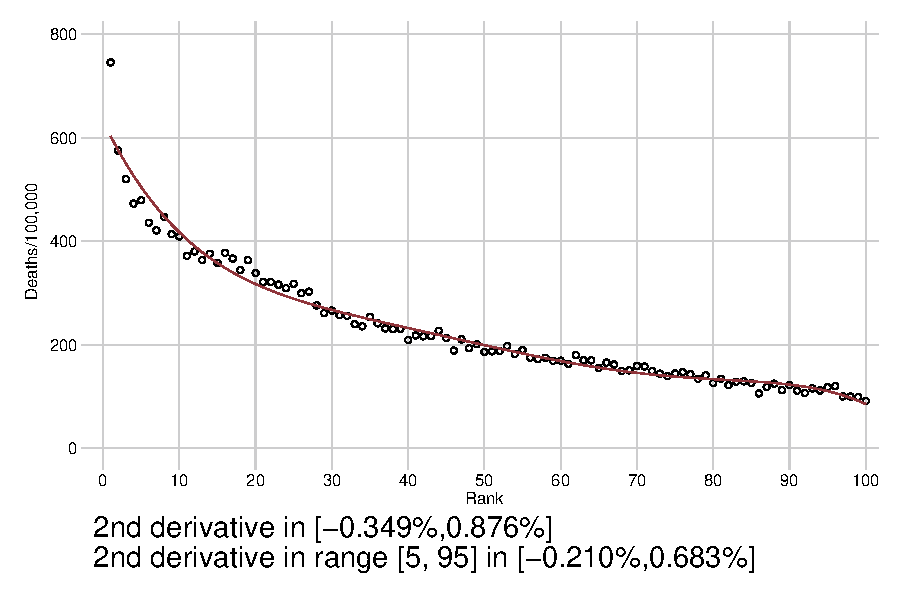
\includegraphics[scale=0.75]{\mortalitypath/polyspline__50_F_2012-2014}
  \end{center}

\begin{center}  
  Panel B: 50--54 Year-Old Men in 2012--2014 
\end{center}
  \begin{center}                                                          %%
      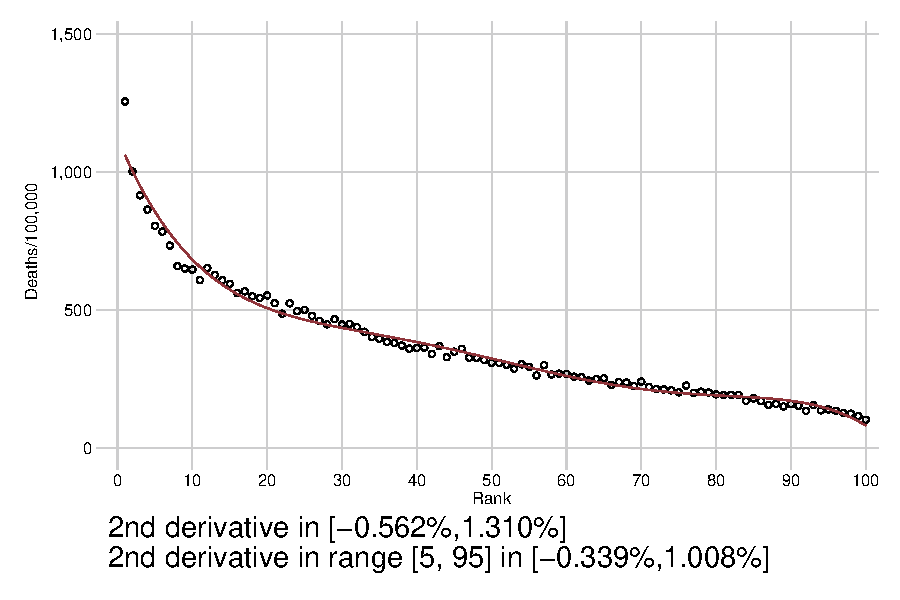
\includegraphics[scale=0.75]{\mortalitypath/polyspline__50_M_2012-2014} %%
  \end{center}                                                            %%
  

  \noindent
  \footnotesize{Figure \ref{fig:mort_poly} presents estimates of
    the conditional expectation function of U.S. mortality given
    income rank, using data from \citet{Chetty2016b}. The CEF is
    fitted using a fifth-order polynomial. The function plots the best
    polynomial fit to the data series, and the circles plot the
    underlying data. The text under the graph shows the range of the
    second derivative, divided by the mean mortality rate in all
    percentiles, across the function's support.}
\end{figure}

% \floatbarrier

\subsection{Comparison with Other Approaches} 
\label{sec:app_comparison} 
\normalsize The selection bias in estimates of mortality change among the less educated is widely recognized and has been examined in other studies. \citet{Meara2008}, \citet{Bound2015}, \citet{Hendi2015}, and \citet{Leive2020} (henceforth MBHL) adjust for this bias by randomly reassigning deaths to different education bins, so that bin sizes are comparable across time. For example, to obtain an estimate of mortality in the bottom quartile of the education distribution in 1992 when 19\% of 50-year-old men are dropouts and an additional 36\% are high school graduates, they would reassign 6/36 = 16.6\% of the high school graduate population and 16.6\% of high school graduate deaths to the bottom bin.

This approach is equivalent to assuming that the conditional expectation function of mortality given latent education rank takes a specific functional form---a step function that is totally flat in each education category, and has a discrete jump at each education boundary. To be concrete, under this assumption, an individual who just barely managed to complete high school (and thus has the lowest latent education rank among high school graduates) has exactly the same implied socioeconomic status and expected mortality risk as a high school graduate who was right at the margin of completing a two year college degree (and thus has the highest latent education rank among high school graduates). Standard human capital theory suggests that the true functional form is not flat in each category---the high school educated individuals who were at the margin of completing some higher education would have had higher socioeconomic status than those who barely made it to high school, and thus lower mortality risk.

This implicit functional form is nevertheless considered a valid functional form in our bounding exercise, which allows arbitrary steps and slope changes at education boundaries. But this functional form underestimates mortality among the least educated in all periods, because it constructs bins by combining dropouts with average high school graduates -- even though the high school graduates with the lowest latent ranks are likely to have higher mortality than average high school graduates.  The downward bias on mortality among the least educated will be the highest when the education-mortality gradient is steep. Because this gradient has steepened over time \citep{Goldring2016}, the downward bias on mortality is higher in 2018 than in 1992, which means that mortality change among the least educated is biased downward when we use this functional form.

Note finally that these other approaches are likely to be increasingly biased when the bin boundary shifts more over time, or when the desired outcome percentiles are very different from the bin boundaries in the raw data, but the estimates from the MBHL function will not reflect this source of error. One reason that few of these authors focus on the very bottom of the education distribution (or the percentiles approximating high school dropouts) is that the large population change in dropouts (among women, from 19\% of the population in 1992 to 8\% in 2018) leads to a substantial potential for bias.  With our approach, in contrast, the bounds reflect the uncertainty in the estimates and become wider in cases like these where bin boundaries have shifted substantially. Our bounds thus accurately convey the uncertainty due to misalignment between desired outcome percentiles and bin boundaries in the data.

The MBHL function generates a mortality estimate among the least educated that is close to our lower bound mortality estimate. Our results are therefore entirely consistent with \citet{Meara2008}, who find that death rates among those with a high school education or less are diverging from those with any college education. We find similar effects for the period up to 2000 studied by \citet{Meara2008}, and show that (i) mortality by education continues to diverge from 2000--2018; and (ii) the bottom 10\% of whites do particularly badly in both periods.

In contrast, \citet{Bound2015} argue that the composition adjustment effectively erases large mortality increases among non-Hispanic whites in the bottom 25\%, though they continue to find average decreases in life expectancy at age 25 among non-Hispanic whites in this education group.  These differences can be reconciled with our finding of substantially rising mortality rates among the least educated non-Hispanic whites. First, as noted in this section, the Bound et al. estimates are at the lower bound of mortality change because of the implicit functional form assumption. Second, we find that mortality increases are most severe among the bottom \textit{10\%}; extending the interval to the bottom 25\% substantially attenuates the estimated mortality change, and makes the functional form bias larger. Third, we focus on middle-age mortality change, because of known problems of age inaccuracy among older ages \citep{Olshansky2012}; trends among individuals aged 70 and older may substantially influence life expectancy and be different from those studied here.

Hendi (2015, 2017) use data from NHIS to argue that mortality is rising for white women without high school education but not white men. We find worse outcomes for both women and men because: (i) the random reassignment approach of Hendi (2015, 2017) biases downward estimates of mortality change; (ii) as noted in detail by Sasson (2017), the NHIS consistently samples a healthier population than that reflected in population vital statistics, and the mortality followup sample sizes are too small to precisely estimate mortality changes for less educated groups. We perform a similar analysis in Appendix~\ref{sec:app_nhis}, showing that while NHIS generates point estimates of lower mortality changes for less educated women (but not men), the estimates are extremely noisy and our estimates are well within the 95\% confidence intervals of the NHIS measures. In some age/education groups, NHIS mortality changes are estimated from just a handful of deaths.

Hendi (2015, 2017) also raise the possibility that over-reporting of education in death statistics may have changed over time, as noted by \citet{Sorlie1996}, leading to underestimates of death rates among older cohorts of dropouts. While we cannot rule out this form of bias, we present a range of evidence in Appendix~\ref{sec:app_robust} (summarized in Section~\ref{sec:robust}) suggesting that misreporting of education in death records cannot explain larges increases in mortality among white men and women.


\newpage 
\clearpage 

\renewcommand{\thetable}{D\arabic{table}}
\renewcommand{\thefigure}{D\arabic{figure}}
\setcounter{table}{0}
\setcounter{figure}{0}

\section{Appendix: Robustness}
\label{sec:app_robust}

\subsection{Loosening the Monotonicity Assumption}
\label{sec:app_nonmon}
\normalsize The results in the body of the paper use an assumption that mortality is weakly monotonically decreasing in the latent education rank. In this section, we explore the sensitivity of the results to loosening this assumption. Using the numerical optimization described in Section \ref{sec:app_numerical}, we alter the monotonicity assumption such that the discrete CEF is permitted to be non-monotonic across at most $m$ rank bins out of 100.

Table~\ref{tab:semimon} shows how the bounds on white male and female mortality change in percentiles 0--10 under values of $m$ ranging from 0 to 100. The case of $m=0$ corresponds to the monotonicity assumption used in the body of the paper and reproduces the results from the main analysis (Figures~\ref{fig:mort_main}A and \ref{fig:mort_main}B in the body of the paper).

Note first that for the 2016--18 results, loosening monotonicity has very little effect. In this period, exactly 10\% of men are high school dropouts, meaning $\mu_0^{10}$ is known. Among women, 8.0\% are dropouts, which gives us $\mu_0^8$; this leaves little room for mortality to depend on functional form assumptions in the bottom 10\%.

In 1992--94, dropouts represent the bottom 17.1\% and 17.4\% for men and women respectively, leaving more uncertainty over the value of mortality in the bottom 10\%. Loosening the monotonicity restrictions in 1992 naturally widens the bounds. Figure \ref{fig:semimon} shows the pair of optimized CEFs that produce the upper and lower bounds for the case of 50--54-year-old white women.

The primary results of rising mortality among both groups are upheld in all cases. The bounds expand moderately up to $m=20$, rising from $[+105\%, +152\%]$ for white women at $m=0$ to $[+67\%, +204\%]$ at $m=20$. As conveyed by the figure, loosening monotonicity entirely results in very implausible functional forms for the CEF. Even the CEFs at $m=20$ are difficult to reconcile with an a priori theory of mortality change, and exhibit higher degrees of non-monotonicity than suggested by the data for any of the subgroups. We therefore view this exercise largely as a demonstration of our method's capability to be adapted to any set of structural assumptions.

Note that if monotonicity and curvature are both totally unrestricted, then much wider bounds are possible, though again we would not consider these to be realistic. For instance, mortality among white men in 1992--94 is known to be 1197 per 100,000 in the bottom 17\%. The mathematical upper bound on mortality in the bottom 10\%, with no structural restrictions, would be given by a mortality rate of 2035/100,000 for percentiles 0--10, and 0/100,000 for percentiles 10--17. While mathematically possible, this function is not a realistic possibility. In our setup, it violates both the monotonicity constraint (since mortality would need to rise with high school completion) and the curvature constraint (since implied mortality falls sharply and discontinuously between 10 and 11).

\begin{table}[H]
  \caption{Mortality Change in the Least Educated 10\% \cnewline Estimates with Variable Non-Monotonicity }

  \begin{center}
    \footnotesize{\begin{tabular}{ccccc}

  \hline
Group &   Non-monotonicity & Mortality & Mortality & Percent \\
      &   Tolerance        & 1992--94      & 2016--18      & Change  \\
  \hline
White Women, Age 50 &  0   & $[613,722]$   & $[1481,1542]$     & $[105.2\%, 151.6\%]$   \\
 &   5   & $[612,742]$   & $[1477,1546]$     & $[99.2\%, 152.6\%]$   \\
 &   10  & $[577,753]$  & $[1477,1553]$   & $[96.1\%, 169.0\%]$  \\
 &   15  & $[524,821]$  & $[1477,1552]$   & $[79.9\%, 196.1\%]$  \\
 &   20  & $[513,885]$  & $[1475,1556]$   & $[66.6\%, 203.5\%]$  \\
%%     &   25  & $$b_f_1992_25_lb$$  & $$b_f_2016_25_ub$$   & $$b_f_diff_25$$  \\
%%     &   30  & $$b_f_1992_30_lb$$  & $$b_f_2016_30_ub$$   & $$b_f_diff_30$$  \\
%%     &   40  & $$b_f_1992_40_lb$$  & $$b_f_2016_40_ub$$   & $$b_f_diff_40$$  \\
%%     &   50  & $[415,928]$  & $[1475,1560]$   & $[59.0\%, 275.9\%]$  \\
 &   100 & $[384,945]$ & $[1475,1562]$ & $[56.0\%, 306.6\%]$ \\
\hline \\
White Men, Age 50 &   0   & $[1200,1394]$   & $[1946,1946]$     & $[39.6\%, 62.2\%]$   \\
 &   5   & $[1200,1427]$   & $[1946,1946]$     & $[36.4\%, 62.2\%]$   \\
 &   10  & $[1182,1528]$  & $[1946,1946]$   & $[27.4\%, 64.7\%]$  \\
 &   15  & $[1161,1590]$  & $[1946,1946]$   & $[22.5\%, 67.7\%]$  \\
 &   20  & $[1101,1635]$  & $[1946,1946]$   & $[19.0\%, 76.9\%]$  \\
%%    &   25  & $$b_m_1992_25_lb$$  & $$b_m_2016_25_ub$$   & $$b_m_diff_25$$  \\
%%    &   30  & $$b_m_1992_30_lb$$  & $$b_m_2016_30_ub$$   & $$b_m_diff_30$$  \\
%%    &   40  & $$b_m_1992_40_lb$$  & $$b_m_2016_40_ub$$   & $$b_m_diff_40$$  \\
%%    &   50  & $[920,1676]$  & $[1946,1946]$   & $[16.2\%, 111.6\%]$  \\
 &   100 & $[874,1713]$ & $[1946,1946]$ & $[13.6\%, 122.7\%]$ \\

  \hline
  
  
\end{tabular}
}
  \end{center}
  \label{tab:semimon}
\end{table}
  \footnotesize{The table shows bounds on mortality and mortality change of white men and women aged 50--54 in the least educated 10\% of the own-gender education distribution. Bounds are calculated under different tolerances for non-monotonic CEFs. The tolerance column indicates the number of rank cells out of 100 where mortality is permitted to be increasing with higher education.}

\begin{figure}[H]
  \caption{Bounds on Mortality in the Bottom 10\%: \cnewline Mortality CEFs under Variable Non-Monotonicity Constraints}
  \label{fig:semimon}
  \begin{center}
    \begin{tabular}{cc}
      \panel\textbf{A. Non-Monotonicity Tolerance = 0} &
      \panel\textbf{B. Non-Monotonicity Tolerance = 5} \\

      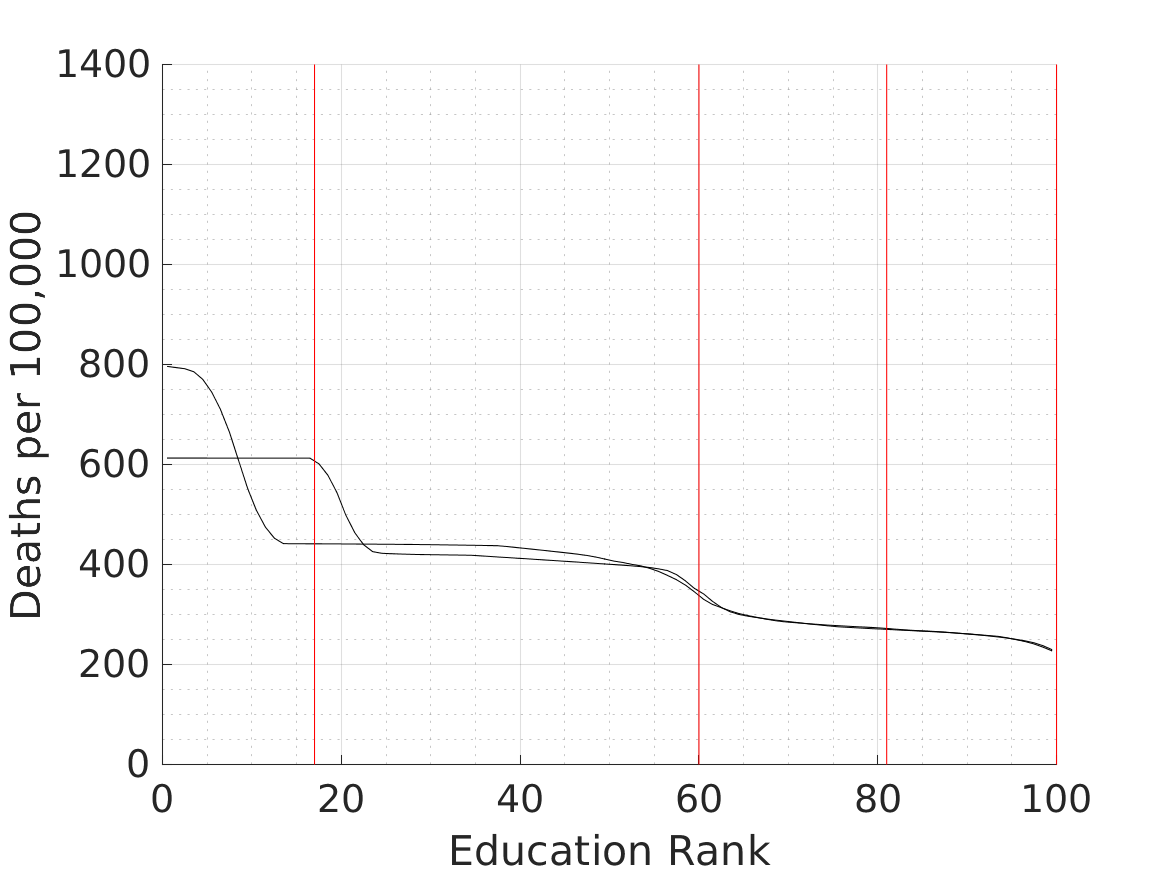
\includegraphics[scale=0.35]{\mortalitypath/f1992_semimon_0.png} &
      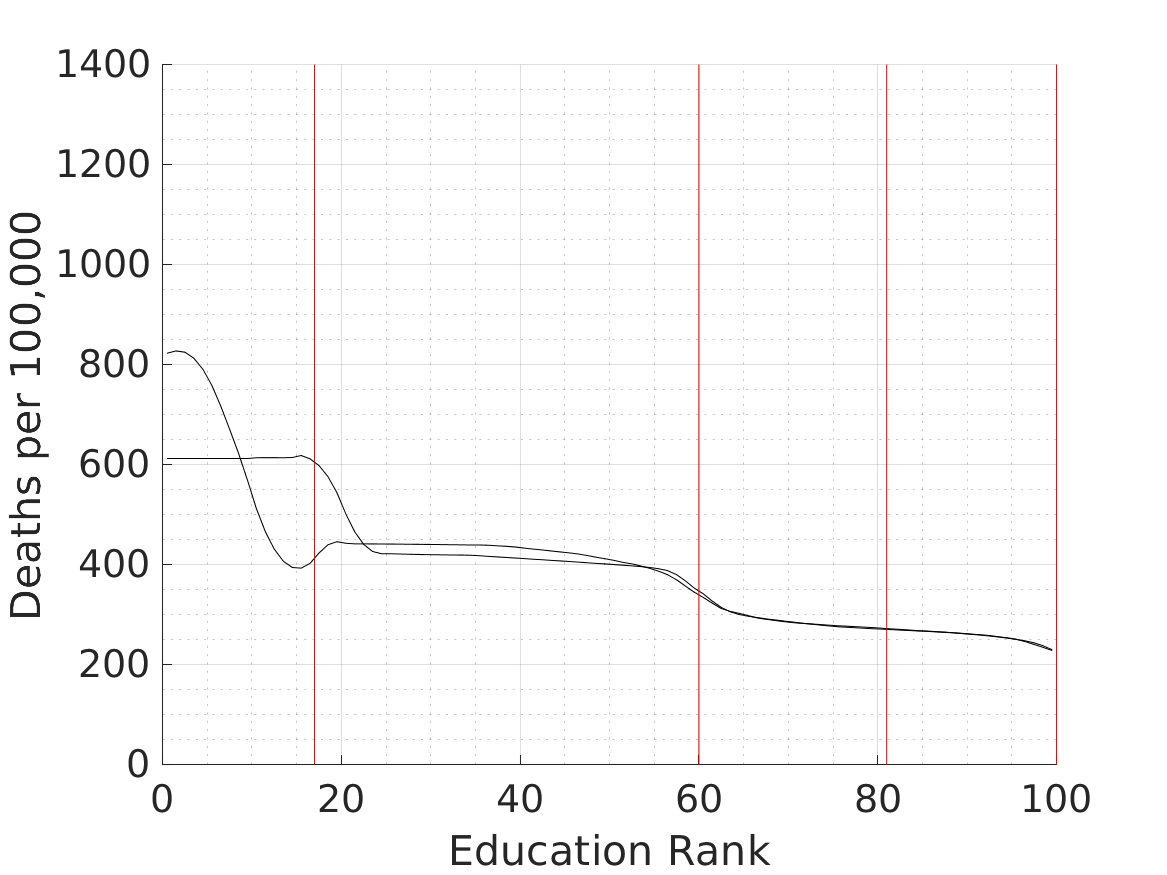
\includegraphics[scale=0.35]{\mortalitypath/f1992_semimon_5.png} \\
      
      \panel\textbf{C. Non-Monotonicity Tolerance = 20} &
      \panel\textbf{D. Non-Monotonicity Tolerance = 100} \\

      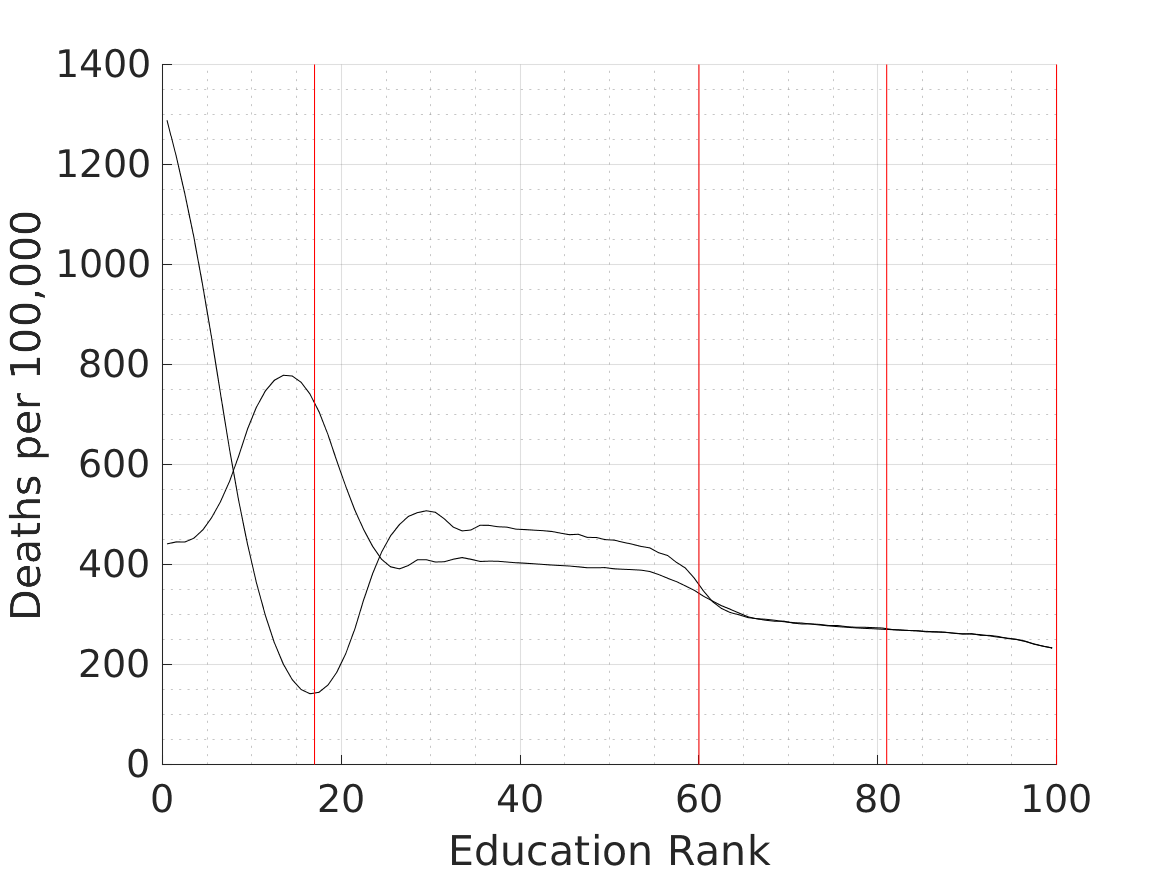
\includegraphics[scale=0.35]{\mortalitypath/f1992_semimon_20.png} &
      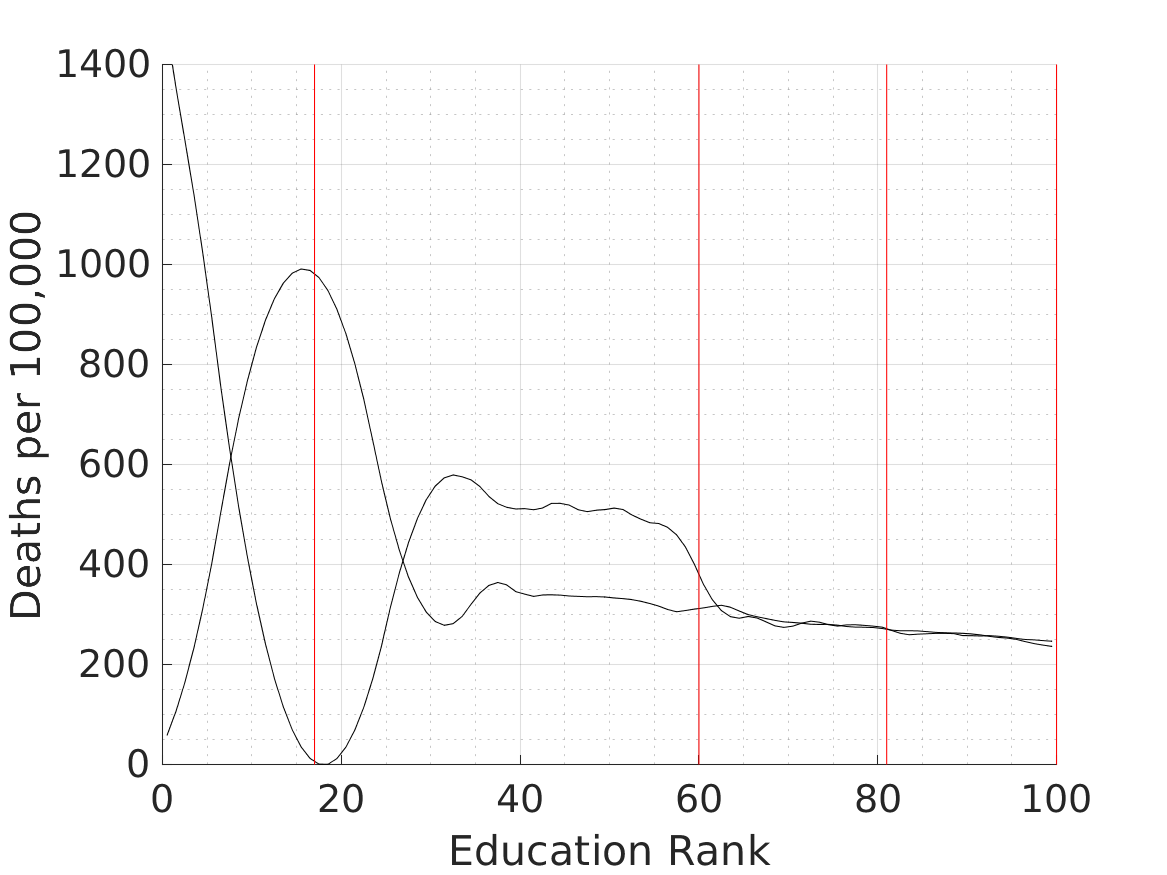
\includegraphics[scale=0.35]{\mortalitypath/f1992_semimon_100.png} \\
      \hline
    \end{tabular}
  \end{center}
  \footnotesize{The figure shows the conditional expectation functions that generate the highest and lowest values of mortality among the least educated 10\%, for 50--54-year-old white women, under different monotonicity assumptions. The tolerance value is the number of rank cells out of 100 where mortality is permitted to be increasing with higher education.}
\end{figure}



\subsection{Robustness to Alternate Specifications and Assumptions}
\label{sec:app_assumptions}
\normalsize \normalsize This section reports changes in mortality from 1992--1994 to 2016--2018 calculated under different assumptions and parameters. We focus on the sensitivity of estimates in Figure \ref{fig:mort_main} for non-Hispanic white women; results for other groups are similarly robust to the specifications here.

\textbf{Percentile Bins Defined in 1992.}  The main figure was calculated using education percentile bins from approximately the middle of the sample in 2003. In that year dropouts accounted for percentiles 0--10, high school graduates for percentiles 10--45, individuals with some college for percentiles 45--70, and individuals with a B.A. or higher accounted for the top 30\%. In 1992, these four education levels respectively represented percentiles 0--17, 17--60, 60--81 and 81--100. Panel A of Figure \ref{fig:robust} shows estimates of mortality change from 1992--94 to 2016--2018 using the latter bin boundaries. The broad patterns of mortality change are the same. Mortality changes are slightly smaller in the bottom group, but this is what we would expect given that the bottom group is now defined as the bottom 17\% rather than the bottom 10\%. The overall divergence of mortality by education is unambiguous.

\vspace{6mm} \textbf{Ranking within Race and Gender.} The body of the paper ranks individuals against members of their own gender. It thus reports, for example, changes in mortality for white women in the bottom 10\% of the female education distribution. An alternate approach is to define percentiles within race and gender, and thus to examine mortality changes for white women in the bottom 10\% of the white women's education distribution. This approach would be sensible if one's relative position in the own-race socioeconomic distribution was an important factor for mortality. Panel B of Figure~\ref{fig:robust} presents the main estimates, where education percentiles are defined within race and gender. The pattern of dramatically rising mortality for whites in the bottom 10\% remains evident. The total increases in mortality are slightly less under this definition, because white education has increased more than black education over this period, but the change in selection bias is small.

\vspace{6mm} \textbf{Alternate Bounding Assumptions.} The main analysis calculated bounds under the assumptions that (i) expected mortality is weakly monotonically declining in latent educational rank for all groups; and (ii) there is an upper bound on the size of kinks or discrete jumps in the expected mortality function.
While these assumptions are sensible and consistent with other
research and data on the expectation of mortality as a function of
education, we can readily relax these assumptions. Although our main
estimates are necessarily less precise under more general assumptions,
none any of the substantive conclusions change. 

Appendix~\ref{sec:app_nonmon} above presents bounds on mortality change as we gradually loosen the monotonicity assumption, and allow mortality to rise with education.

Panel C of Figure~\ref{fig:robust} presents results when we allow the
mortality function to have discrete jumps or kinks of any size when
crossing educational boundaries, for example, when crossing the
threshold of high school completion. Thus Panel C addresses concerns
about sheepskin effects by permitting (but not imposing) mortality to
fall discontinuously at the margin of completing a given education
level. 

Panel D removes the curvature restriction entirely; in this specification, the CEF can have discrete kinks or jumps at any point in the education rank distribution, though it must remain monotonic. In both cases, the key result of substantial mortality gain among the least educated is robust. The other findings of the paper---education divergence among black men and women, and the patterns of deaths of despair---are similarly robust to these specifications.

%%%%%%%%%%%%%%%%%%%%%%%%%%%%%%%%%%%%%%%%%%%%%%
% Figure: Causes of Death -- 1992 Boundaries %
%%%%%%%%%%%%%%%%%%%%%%%%%%%%%%%%%%%%%%%%%%%%%%
\begin{figure}[H]
  \caption{Change in non-Hispanic White Female Mortality: Sensitivity Analysis} \thispagestyle{empty}
  \label{fig:robust}

  \begin{center}
    \vspace{-.6cm} Panel A: 1992 Percentile Boundaries
  \end{center}
  \vspace{-1.4cm}
  \begin{center}
    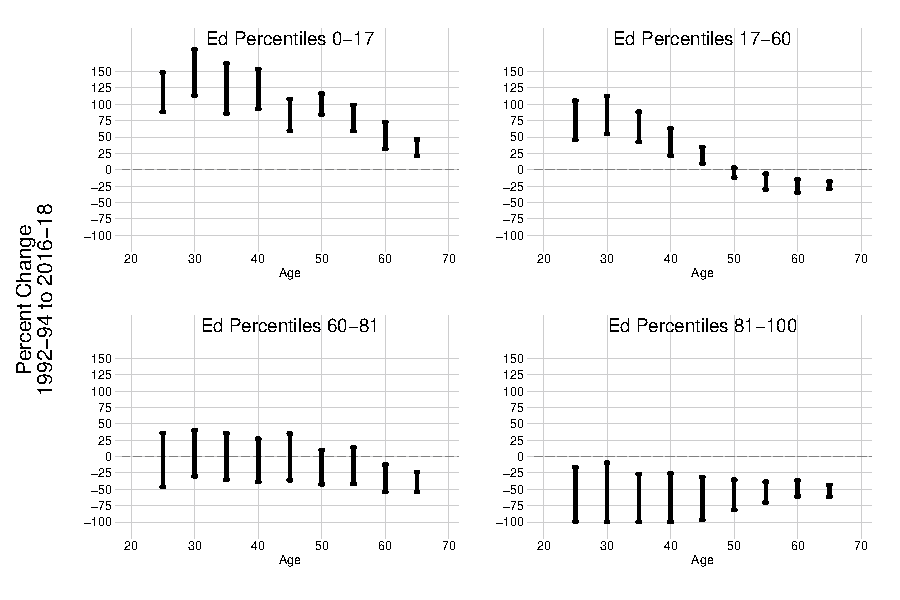
\includegraphics[scale=1.1]{\mortalitypath/causes-1992-2-1} &
  \end{center}

  \begin{center}
    \vspace{-.6cm} Panel B: Within Race-Gender Percentiles
  \end{center}
  \vspace{-1.4cm}
  \begin{center}
    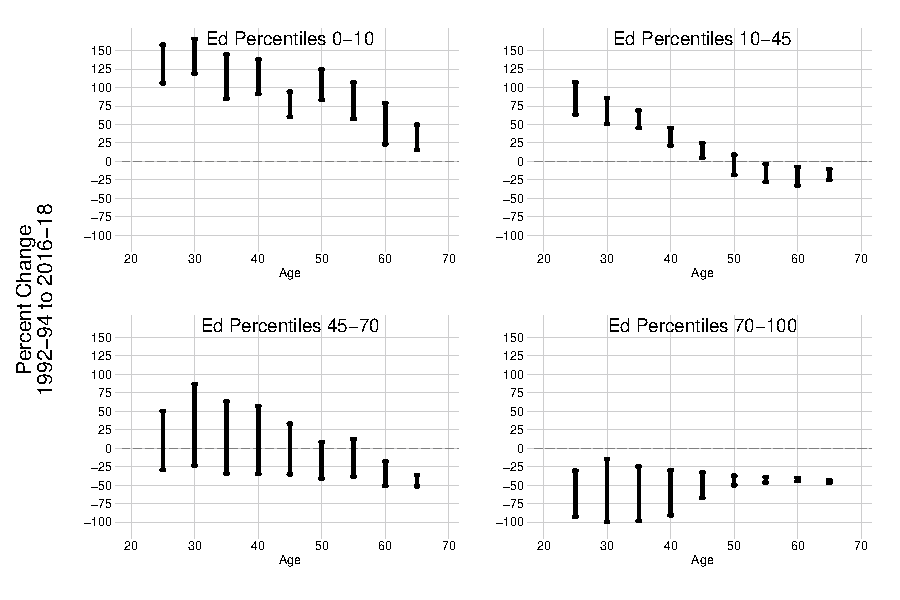
\includegraphics[scale=1.1]{\mortalitypath/causes-racesex-2-1} \\
  \end{center}
\end{figure}

\begin{figure}[H]\ContinuedFloat
  \caption{Change in non-Hispanic White Female Mortality: Sensitivity Analysis (Continued)} \thispagestyle{empty}
  \begin{center}
    \vspace{-.6cm} Panel C: Allow Sheepskin Effects
  \end{center}
  %\vspace{-1.4cm}
  \begin{center}
    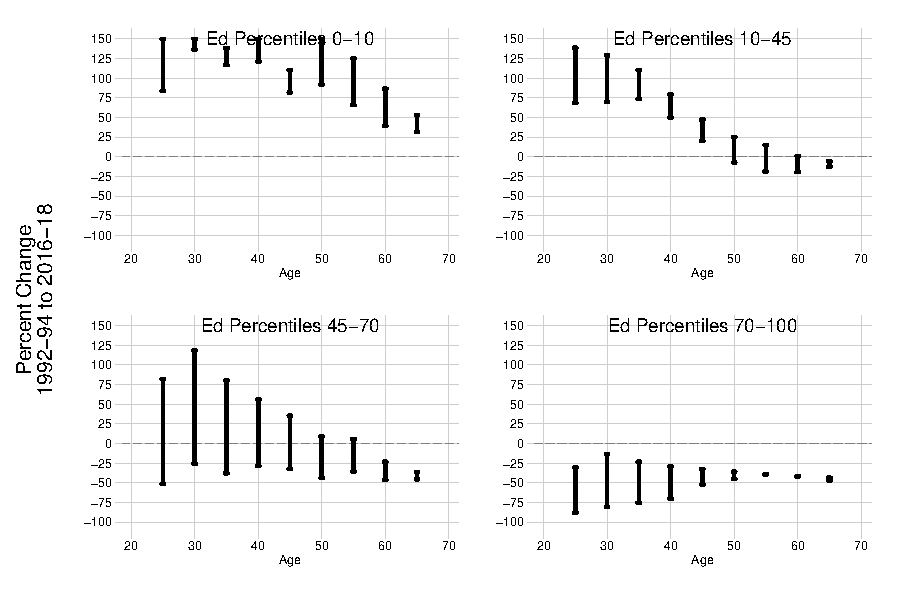
\includegraphics[scale=0.78]{\mortalitypath/causes-mon-step-2-1} \\
  \end{center}

  \begin{center}
    \vspace{-.6cm} Panel D: No Curvature Constraint
  \end{center}
  %\vspace{-1.4cm}
  \begin{center}
    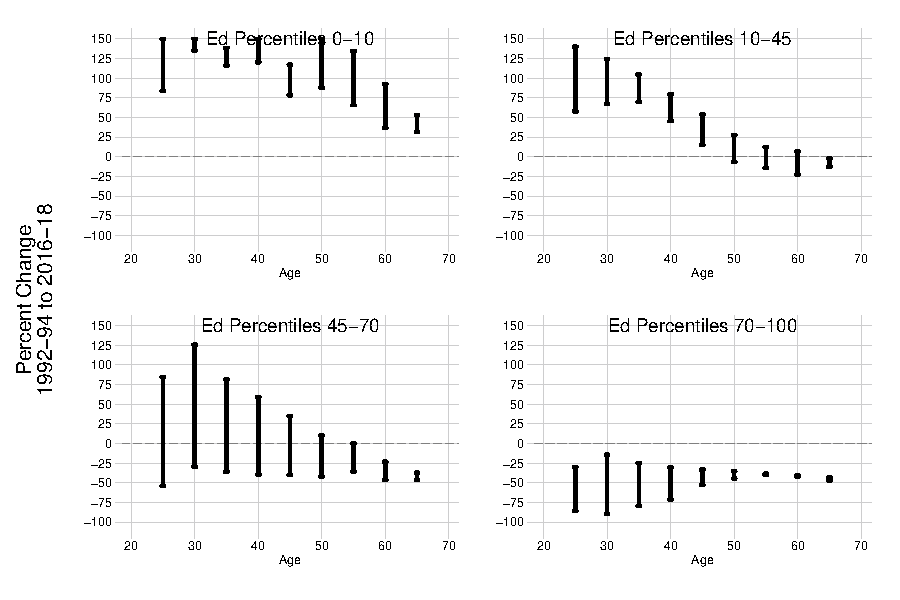
\includegraphics[scale=0.78]{\mortalitypath/causes-nof2-2-1} \\
  \end{center}
\end{figure}
\vspace{-1cm} \tiny{Note: The figure shows bounds on mortality change from 1992--1994 to 2016--2018, for non-Hispanic white women, by age and percentile education bin, under alternate assumptions from the main body of the paper. The figure is analogous to Panel A of Figure~\ref{fig:mort_main}, but with different bounding assumptions. Panel A defines education bins boundaries according to education levels in 1992--1994. Panel B defines an individual's education percentile according to the individual's rank in the own-race and own-gender education distribution, rather than in the own-gender education distribution. Panel C allows sheepskin effects, by allowing kinks and discrete jumps at education boundaries (e.g. the rank separating dropouts from high school completers). Panel D estimates bounds on mortality without restricting the curvature of the mortality-education CEF. The lines show the bounded set containing the percentage change in the mortality rate from 1992--1994 to 2016--2018 for the given group.}



\clearpage
\subsection{Changing Racial Composition} 
\label{sec:app_race_distrib} 
\normalsize 
This section examines the hypothesis that relative socioeconomic
status \textit{within} education bins has changed for blacks relative
to whites during the study period. This kind of change could bias our
estimates of mortality change, because we assume that the latent
education ranks of blacks and whites \textit{within} the bottom 10\%
(and within other percentile groups) have not changed during the study
period. For example, if whites within the bottom 10\% were clustered
at the top of this percentile bin in 1992--94 and at the bottom of this
bin in 2016--18, then we would expect their measured mortality to rise
even if the underlying mortality-education-rank CEF is unchanged.  To
be concrete, suppose the mean white woman, conditional on being in the
bottom 10\% of all women, moved from the 7th percentile to the 3rd
percentile. Then comparing average mortality among white women in the
bottom 10\% could still be subject to selection bias, even in our
constant composition estimates, because the average white woman in the
bottom 10\% would be more negatively selected over time.

Note that Panel B of Figure~\ref{fig:robust} already rules this out as a
primary explanation for rising white mortality, by showing that
mortality is rising for the bottom 10\% of whites, not just for whites in
the bottom 10\% of the national education distribution. Nevertheless,
in this section we explore the possibility that the relative status of
whites in the bottom 10\% of the entire educational distribution has
shifted relative to blacks.

Because education data is interval censored (i.e. we only know that
someone is a high school dropout, but we do not observe how close they
were to completing high school), we cannot measure the education
percentile more precisely. However, we can examine whether the
socioeconomic status of white dropouts has changed relative to black
dropouts on other measures. We focus on income as measured in the
Current Population Survey.

First, we use the granular information on incomes in the CPS to rank
all people by income within each gender, age and education bin in each
year. We then compute the mean income rank for whites and blacks
within each of the four education groups used in the body of the
paper.  Figure~\ref{fig:income_ranks} plots the results of this
exercise for women and men aged 50--54. The figures show that mean
income ranks for blacks and whites, conditional on education level,
have remained stable over time. Among women, black and white dropouts
have approximately equal income rank throughout the sample
period. Among high school graduates, the relative status of whites is
increasing relative to that of blacks, which would bias us
\textit{against} finding increases in mortality. Among men, whites
have higher average income ranks within every education bin, but their
relative advantage is stable over time.  Changing relative latent
education rank \textit{within} observed education bins therefore
cannot explain any of the rise in mortality of white dropouts.
\clearpage
\begin{figure}[H]
  \caption{Average Income Ranks for 50--54 year old whites and blacks}
  \label{fig:income_ranks}
  \begin{center}
    Panel A: Women \\
      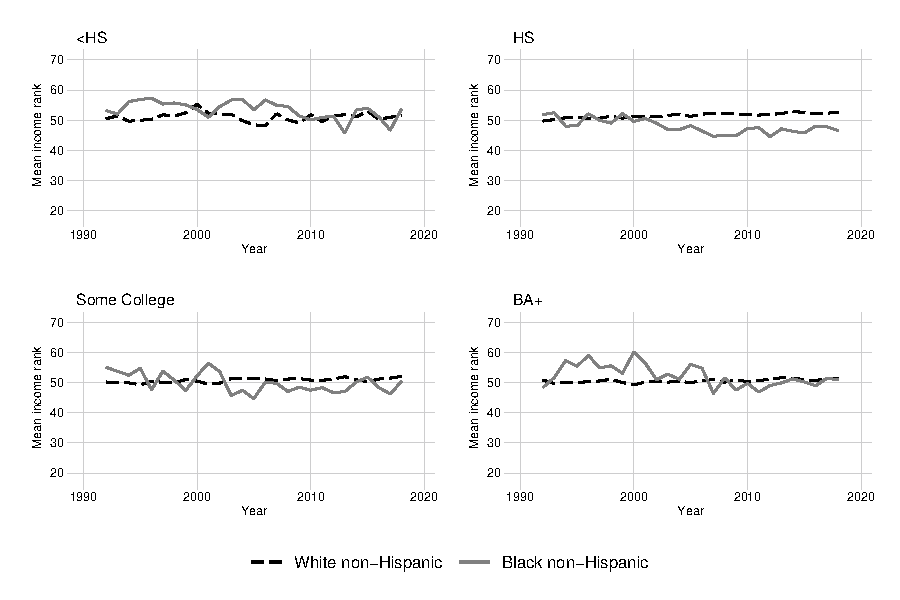
\includegraphics[scale=.75]{\mortalitypath/mean_within_rank_50_2_comb} \\
  \end{center}
  \begin{center}
    Panel B: Men \\
      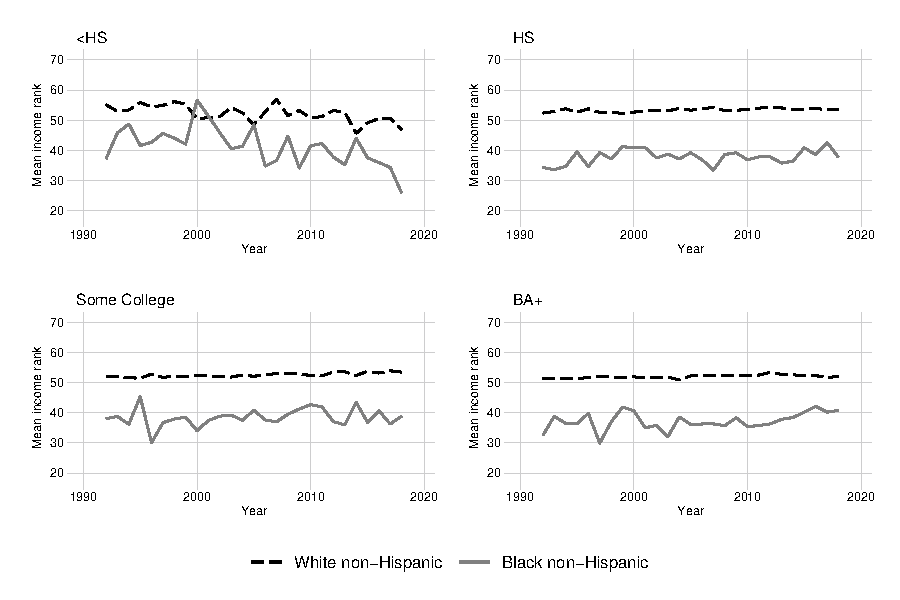
\includegraphics[scale=.75]{\mortalitypath/mean_within_rank_50_1_comb} \\
  \end{center}
\end{figure}

\scriptsize{ Note: The figure shows the average income rank within
  age, gender and education bins for non-Hispanic white and
  non-Hispanic black men and women at different education levels. Source: CPS.}


\clearpage
\subsection{Measurement Error in Race/Ethnicity} 
\label{sec:app_hisp}
\normalsize A concern that has arisen with the estimation of mortality change in the United States among white and black groups is that reporting patterns for Hispanic identity may have changed over recent decades. The Hispanic population of the U.S. has higher in- and out-migration, making mortality estimates for this group more difficult to measure \citep{Markides2005}.  Hispanics also have considerably lower mortality rates than other groups \citep{Palloni2004,Markides2005}. If patterns of Hispanic reporting change over time, and especially if they change differentially across the Current Population Survey and the Vital Statistics databases, then estimates of mortality change for non-Hispanics could be biased.

In this section, we consider and rule out two alternative hypotheses for the measured rise in non-Hispanic white mortality. First, survey questions change subtly over time; for example, the Census permitted people to check multiple race boxes starting in 2000 \citep{Currie2018}. We show that there are no discontinuities in the combined population records for non-Hispanic white or black populations in our sample, suggesting multiple race reporting is not substantially biasing mortality estimates.

Second, populations' attitudes about their own racial/ethnic identity may change over time. The same person might be more likely to report herself as a given race/ethnicity in 2018 than in 1992. Because Hispanics have lower mortality rates, if white Hispanics are more likely to report Hispanic identity over time in surveys, this phenomenon could bias the non-Hispanic mortality trend upward. We conduct a bounding exercise that shows that even if an implausibly large number of whites changed their identity to Hispanic, there would still be large mortality gains among less educated non-Hispanic whites.

Finally, average misalignment between Hispanic identification on death records and in census counts would not bias mortality estimates unless the error rate changed between 1992 and 2018. Further, researchers have examined potential misreporting of Hispanic identity on death certificates, and have found that reporting of identity on death certificates is in fact reliable and consistent with census data, with error rates consistently falling below 10\%, which is too low to explain the patterns described in this paper \citep{Rosenberg1999,Arias2008,Arias2010,Ruiz2013}.

\vspace{6mm} \textbf{Changes in survey questions.} The option to check
more than one race box in the 2000 Census has the potential to change
the share of the population that reports as any given race
\citep{Currie2018}. The CPS question on race changed in 2003, while
the question in the ACS (which we use only to calculate the
institutionalized population) changed in 2008.  Figure \ref{fig:pops}
plots the total population in our dataset by age and race. There is
clearly no large discontinuous change in the population of any group
in either of these years, suggesting that the option to check multiple
races in these national surveys cannot explain the secular trend in
rising mortality among the least educated white non-Hispanics. Note
also that only 5\% of white 20-year-olds in the 2010 Census report
multiple races \citep{Currie2018}. This number drops to less than 2\%
among white 50-year-olds. This is thus unlikely to be a major concern.

\vspace{6mm}

\textbf{Differences between the Census/CPS and NCHS reporting.} A
separate concern is that Hispanic identity could be reported
differently on death certificates and in Census counts. Misreporting
of ethnic identity on death certificates on average would not affect
our findings on mortality \textit{changes} unless the frequency of
misreporting changes substantially during the sample
period. For instance, to create an upward bias in mortality change
among non-Hispanic whites, Hispanic identity could be reported
correctly on death certificates in 1992 but substantially underreported
in 2018. In that case, there must be only small changes in accuracy of
reporting in the CPS. 

To test the extent to which changes in reporting of Hispanic identity could influence mortality estimates among non-Hispanic white mortality, we simulated misreporting in the data, focusing on non-Hispanic white women aged 50--54 in the least educated 10\%. Specifically, we assumed that X\% of white Hispanics in 2016--18 would have reported themselves as non-Hispanic white in 1992--94. We therefore reassigned X\% of white Hispanic deaths to be counted as white non-Hispanic deaths in 2016--18, and then recalculated bounds on mortality change from 1992--94 to 2016--18.  Panels A and B of Figure \ref{fig:hisp_changes} plot the results of this exercise for non-Hispanic white women and men respectively. Even in the extreme case where 20\% of white non-Hispanic female deaths in 2016--18 would have been reported as Hispanic deaths in 1992--94, we would still detect an increase in mortality of [397, 590] deaths per 100,000 among the bottom 10\%, putting the lower bound on mortality increase at 65\%. This example shows that even an extreme amount of misreporting could not drive our findings for the least educated group; however, note that estimates suggest the true amount of this kind of misreporting is much smaller than this extreme case \citep{Rosenberg1999,Arias2008,Arias2010,Ruiz2013}.

\begin{figure}[H]
  \caption{Population Counts by Group}
  \label{fig:pops}
  \begin{center}
    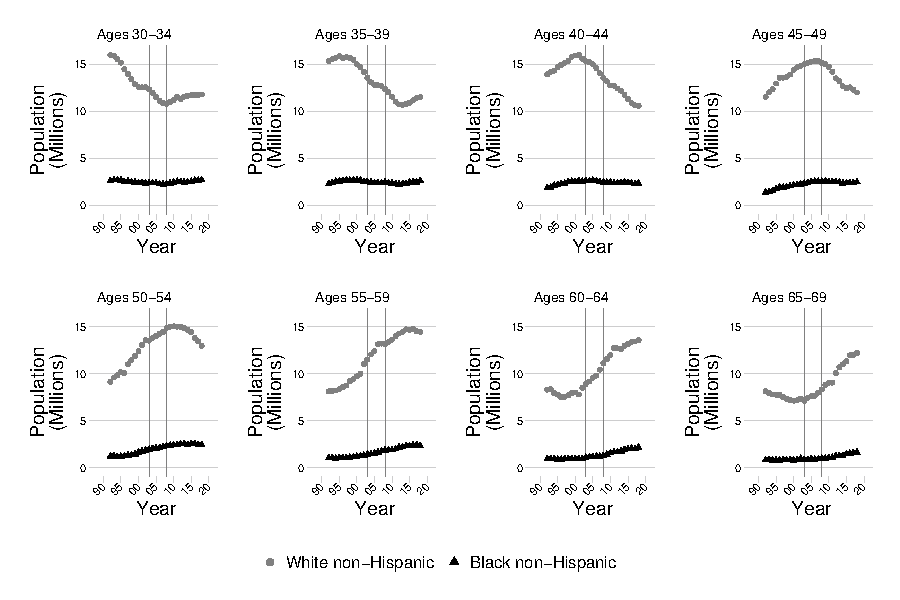
\includegraphics[scale=1.2]{\mortalitypath/total_pops} \\
  \end{center}
\end{figure}
\scriptsize{Note: the figure shows the population in each 5-year age bin of black and white non-Hispanics according to the CPS / ACS over the study sample period.}

\begin{figure}[H]
  \caption{Mortality Changes with Simulated Measurement Error}
  \label{fig:hisp_changes}
  \begin{center}
    \begin{tabular}{c}
      \small{Panel A: Non-Hispanic White Women Ages 50--54} \\ 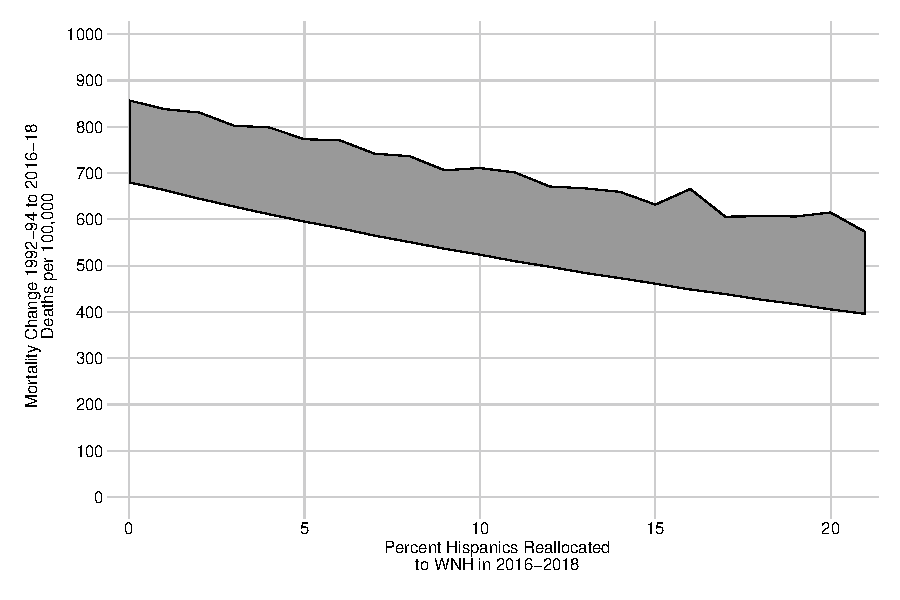
\includegraphics[scale=.75]{\mortalitypath/hisp_shift_2} \\ \small{Panel B: Non-Hispanic White Men Ages 50--54} \\ 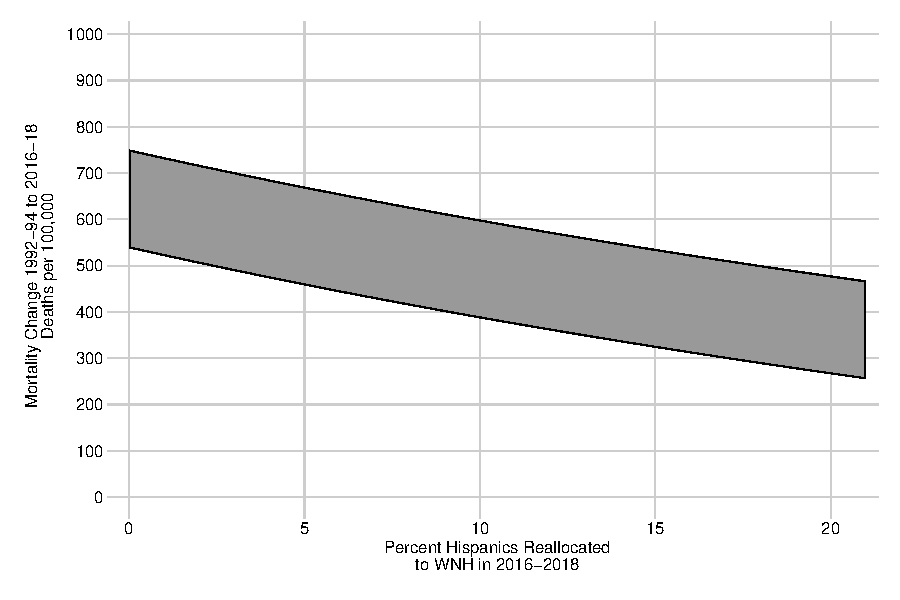
\includegraphics[scale=.75]{\mortalitypath/hisp_shift_1}
    \end{tabular}
  \end{center}
\end{figure}
\scriptsize{Note: The figure displays the sensitivity of mortality estimates to measurement error in ethnicity. The figure shows how primary mortality change estimates change if we recode white Hispanic deaths in 2016--18 to white non-Hispanic deaths, leaving reporting in 1992--94 and population totals unchanged. The X axis shows the percentage of Hispanic deaths recoded as non-Hispanic deaths under each scenario. The Y axis shows bounds on mortality change from 1992--1994 to 2016--2018 among non-Hispanic white men and women aged 50--54 in the least educated 10\%, under each different recoding. Bounds are otherwise calculated as in the body of the paper.}


\clearpage
\subsection{Analysis of Measurement Error Using Synthetic CPS Cohorts}
\label{sec:app_cps_cohorts}
\normalsize This section conducts an exercise to determine whether misreporting of education can explain our estimates of rising mortality among the least educated whites. Specifically, we examine whether changes in CPS cohort sizes are consistent with our mortality estimates. For instance, if we conclude from vital statistics that 5\% of dropouts in a certain cohort die in a given year, then we expect that cohort to shrink by about 5\% in the following year, after adjusting for other factors that can change cohort size. This approach addresses the concern that if CPS respondents increasingly inflate their level of education (\textit{i.e.} report that they have completed high school when in fact they did not), then the denominator of the mortality rate (the estimated number of high school dropouts) would be increasingly biased downward over time, causing us to overestimate mortality change.

We will put an upper bound on this source of bias by studying the size of a synthetic cohort of dropouts and high school completers in the CPS. The size of a cohort of white high school dropouts can change over time for five reasons: (i) deaths; (ii) migration; (iii) continuing education; (iv) false reports of continuing education; or (v) some report that they are Hispanic, even though they would not have reported this in the past.  We calculate an upper limit on the share of individuals who are exiting the sample for reporting reasons; this gives us a bound on the combined bias caused by misreporting of education and ethnicity status in the mortality rate.

We measure the death rate in every period, and we assume that net migration of non-Hispanic middle-aged whites is small enough to ignore. We also estimate the number of individuals passing the GED, which is the primary form of continuing education for individuals who did not complete high school. We obtained the number of GED passers from 1992 to 2013 from the GED Testing Service.\footnote{For a sample report, see the 2009 GED Testing Program Statistical Report, which we downloaded from https://files.eric.ed.gov/fulltext/ED512301.pdf. Due to the absence of more recent data, we use 2015 as a terminal year in the CPS and assume the number of GED passers in 2014 and 2015 is the same as in 2013. Alternate assumptions do not materially affect the results.} The number of passers is disaggregated by 5- or 10-year age group; the GED Testing Service also reports the share of passers who are female and the share who are white. The number of passers is not further disaggregated either into single-year age bins or bins describing age * female or age * race. We therefore assume that the number of passers is distributed uniformly across ages within age bins, and that the female and white shares are the same at all ages. We expect that these assumptions will bias downward our estimates of white female passers at higher ages, as women may be more likely than men to delay continuing education due to pregnancy.

Given our estimate of the number of GED passers and our estimate of the mortality rate, we can predict how the size of a synthetic CPS cohort of high school dropouts will evolve over time. Any discrepancy between our predicted cohort size and the actual cohort size will be driven by migration (which we expect is small), continuing education in a form other than the GED, false reporting of continuing education, or change in reporting of ethnicity. The discrepancy is therefore an upper bound on the mismeasurement of mortality due to individuals exiting the sample due to misleading reporting of education or ethnicity.

Figure~\ref{fig:cps_cohorts_dropouts} presents the results. The top left panel shows the analysis for non-Hispanic white female dropouts. The gray squares show the CPS population of white female dropouts in the 1950--54 birth cohort, approximately the middle 5-year birth cohort in our study. Their population falls over time due to the five factors above. The black dot-dash line is a linear trend fit to the gray points to eliminate year-on-year noise. The dashed blue line shows how the size of this cohort would have evolved over time from mortality alone, beginning at the CPS trend line in 1992, based on our estimates from the NCHS. The red line shows how this cohort would have evolved when we count deaths and GED completions. In 2015, the gap between the linearized CPS cohort size and the predicted cohort size is 8.0\%. Assuming that migration in this cohort is small, this gap is an upper bound on the error in our population count that arises from false reporting of high school completion or changing in reporting of Hispanic ethnicity.

The remaining panels of the figure show the same result for white men, and for white women and men in the 1960--64 birth cohorts. Continuing education explains more of the change in cohort size for the younger 1960--64 birth cohort because individuals are more likely to complete GEDs at younger ages. The potential biases for men are smaller than for women. The potential bias is highest for women in the 1960--64 birth cohort, with a discrepancy of 23.6\% between the CPS population and our predicted population. One factor that could explain this discrepancy is the possibility that women are more likely to take the GED later in life than men because of early pregnancies. Our GED passing numbers did not report age profiles for men and women separately, so we had to assume that men and women are equally likely to take the exam in their thirties and forties. If men are more likely to take the exam in their teens and twenties and women are more likely to take it later in life, then our predicted measures would be even closer to the true series for both men and for women.

Nevertheless, for the sake of argument, we can consider how our mortality change measures would change if our mortality estimates in 2016--18 are biased upward by the worst case estimate of 23.6\%.\footnote{We use 2016--18 as the comparison period, even though we only calculated bias up to 2015 due to availability of the GED data.}  We estimate that 50--54-year-old women (corresponding to the 1960--64 birth cohort in 2016--18) in the least educated 10\% experienced mortality increases of 100--150\% from 1992--94 to 2016--18. If we underestimated the population of white female dropouts in this birth cohort by 23.6\% in 2016--18, the corrected mortality change would be an increase of 62--102\%. While this number is smaller, it is still considerably higher than the mortality change estimate in the next education percentile group--- among similarly-aged women in the 10th to 45th percentiles, we estimate mortality change between -6\% and +20\%.

These worst case assumptions are implausible for three reasons. First, the calculation above uses the discrepancy for the 1960--64 birth cohort, which is among the largest in our sample; among women in the 1950--54 birth cohort, assuming the maximum bias would bring mortality change down only from 132--149\% to 115--131\%. Among men, the bias is less than 10\% across all age groups. Second, as noted above, women may be disproportionately likely to complete the GED at higher ages, bringing down the potential bias. Last, there are other mechanisms for individuals to obtain continuing education after dropping out of high school; we are only able to count the GED, and thus incorrectly attributed other schooling to bias. All these reasons suggest we have overstated the potential bias. Nevertheless, even if we make these worst case assumptions, the overall finding of disproportionately rising mortality among the least educated holds up.

Finally, Figure~\ref{fig:cps_cohorts_hs} shows similar graphs documenting the change in the size of synthetic CPS cohorts of white high school completers. For these groups, we can only predict population change due to mortality, because we could not obtain population counts of the number of whites obtaining any sort of 2- or 4-year degree by year and age. Nevertheless, even without counting continuing education, the potential discrepancies are very small and within the range that could be plausibly explained entirely by continuing education. In short, false reporting of education in the CPS cannot come close to driving the main results of substantial mortality increases among the least educated whites.

\begin{landscape}

\begin{figure}[H]
  \caption{Bounding Measurement Error in CPS Dropout Counts}
  \label{fig:cps_cohorts_dropouts}
  \begin{center}
    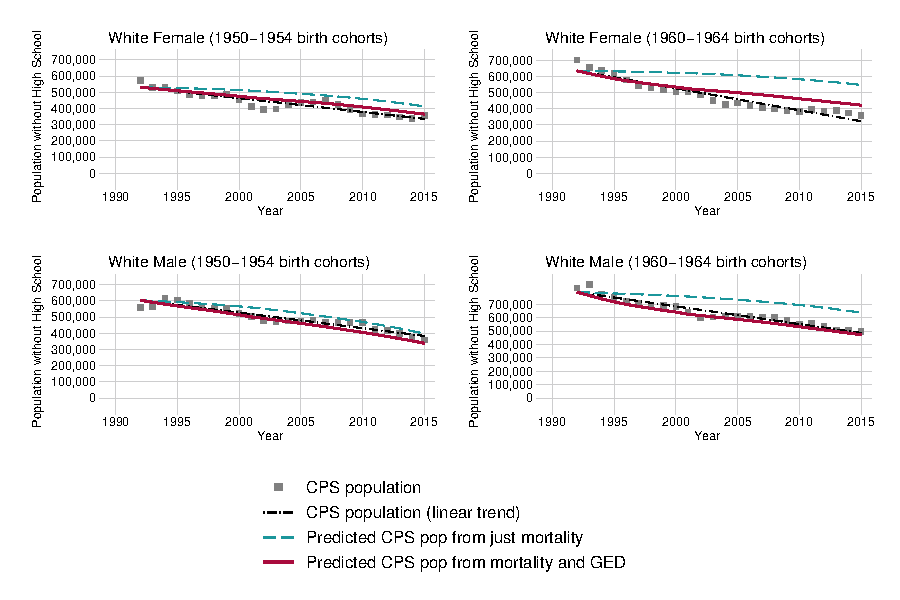
\includegraphics[scale=1.18]{\mortalitypath/cps_pred_all_dropout} \\
  \end{center}
\end{figure}
\scriptsize{The figure displays the population in selected cohorts of
  CPS dropouts. These are compared with the predicted population based
  on measured mortality and GED completion.  The gray points show the
  counts of members of each gender/education group in each round of
  the CPS. The dot-dash black line is a linear trend fit to the gray points to
  eliminate year-on-year noise. The dashed blue lines begin at the
  CPS trend line in 1992, and show how the CPS population  
  would have evolved from mortality alone. The solid red line shows
  how the CPS population would have evolved from mortality and GED
  completion only.}

\begin{figure}[H]
  \caption{Bounding Measurement Error in CPS High School Completer Counts}
  \label{fig:cps_cohorts_hs}
  \begin{center}
    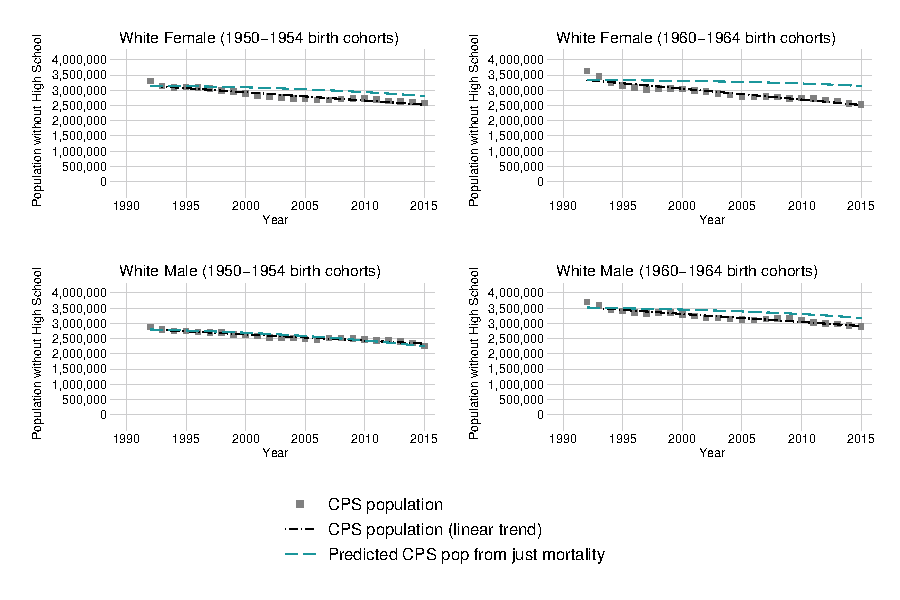
\includegraphics[scale=1.17]{\mortalitypath/cps_pred_all_hs} \\
  \end{center}
\end{figure}
\scriptsize{The figure displays the population in selected cohorts of
  CPS high school completers. These are compared with the predicted
  population based on measured mortality.  The gray
  points show the counts of members of each gender/education group in
  each round of the CPS. The dot-dash black line is a linear trend fit
  to the gray points to eliminate year-on-year noise. The dashed blue
  lines begin at the CPS trend line in 1992, and show how the CPS
  population would have evolved from mortality alone.}
\end{landscape}


\clearpage
\subsection{Comparison with National Health Interview Survey}
\label{sec:app_nhis}
\normalsize In this section, we use an alternate data source to validate the
findings in the body of the paper. We use the National Health
Interview Survey (NHIS), which is an annual repeated cross-section
survey of about 35,000 households and 87,000 individuals. Mortality
rates can be calculated directly from the NHIS, because NHIS records
are intermittently linked to death certificate records from the
National Death Index. We can therefore estimate a population subgroup
mortality rate as the share of individuals who are deceased in a given
followup period.

Because mortality rates and education/ethnicity are all measured for
the same individuals, there is no possibility of inconsistent measurement of ethnicity or education between death counts and population counts. For instance,
if some individuals without a high school education report that they
have a high school education, both their deaths and their population
will be counted among the high school group. This may create a small
bias if mortality is correlated with misreporting, but it will be
considerably less bias than if their deaths are counted in the dropout
group and their population is counted in the high school completion
group.  This said, NHIS-based measures of mortality slightly
underestimate aggregate mortality relative to vital statistics data,
especially for older white women, because the NHIS sample population appears to be more healthy than average \citep{ingram2008}.

We obtained public NHIS data with mortality followup for
NHIS participants linked to death records
through 2015. NHIS interviews occur
throughout the year.\footnote{The sample of deaths in the year following the NHIS
  survey is extremely small. In some of our subgroups, there were zero
  deaths reported in the shortest followup periods.} We aggregated
results across all ages using the standardized U.S. population
distribution, as in Section~\ref{sec:all_ages}. Because our aim in
this section is to validate the raw mortality estimates from the NCHS,
we present raw mortality change for education levels, rather than
bounding the mortality change in constant education percentiles.

Figure~\ref{fig:nhis_mort} below compares estimates of annualized
mortality change in the NHIS vs. our estimates from the NCHS for the
four key groups in our study: non-Hispanic white female dropouts and
high school completers, and non-Hispanic white male dropouts and high
school completers. Mortality change in the NHIS is calculated from
the average mortality in periods 1997--1999 to the last period in which the $n$-year mortality rate can be
calculated. For example, we can compute 1-year mortality for the 2014
data, 2-year mortality for the 2013 data, etc. 

The red points in Figure~\ref{fig:nhis_mort} show NHIS mortality estimates with 95\%
confidence intervals. Even with the 6-year followup period, the NHIS
sample is too small to precisely estimate mortality change over the
sample period. Most point estimates are very close to our mortality
change estimates from NCHS data (indicated by the dashed green line),
but in many cases the NHIS confidence interval includes both zero and
our measure. In almost all cases, our NCHS measure of mortality change
is within one standard error of the NHIS estimate and they are particularly close for the largest sample mortality followup in NHIS (6 years).\footnote{Compared with our
  results, NHIS calculates slightly higher mortality increases for high school completers and slightly lower for dropouts, but the opposite interpretation also falls within the confidence interval. The NHIS estimates are just not precise enough to make any clear statement about the difference between these groups.}

\textbf{Health status.} NHIS estimates of mortality are imprecise because the number of
middle-aged white dropouts in the sample who die is very small. We can
obtain more precise estimates of health status, which is reported by
all respondents. NHIS respondents are asked to report their perception
of their own health on a five point scale, where one reflects very
good health, and five reflects very bad health. In
Figure~\ref{fig:nhis_health}, we show the annualized change
in self-reported health status from 1997 to 2014 at each age and
education level, plotted with a lowess smoother.

The left panel shows the result for non-Hispanic white women. At most
ages, dropouts have experienced worse health declines than members of
any other group. Among 40--60-year-old women, self-reported health
status has gotten 0.0175 points worse \textit{per year}, or 0.2 points
worse on a 5 point scale from 1997 to 2009. The age pattern of the
health decline closely matches our mortality results in
Figure~\ref{fig:mort_main}, with the greatest divergence between
dropouts and high school graduates occurring between ages 40 and
60. We observe less change in the education-health gradient among men,
but dropouts suffer the worst relative deterioration in health between ages
50--70, corresponding exactly to the ages where we document the
greatest differential increases in mortality among the bottom 10\% in
Figure~\ref{fig:mort_main}.

In conclusion, measures of mortality and self-reported health in the
NHIS are broadly consistent with our findings of increased
mortality among middle-aged whites in the least educated
10\%. These NHIS measures are less precise than the vital statistics
mortality data, but they do not suffer from any division bias that
could be caused by changes in how individuals respond to questions
about their education or ethnicity over time.

\begin{figure}[H]
  \caption{Annualized Mortality Change Estimates from NHIS and from NCHS (1997--2015)}
  \label{fig:nhis_mort}
  \begin{center}
    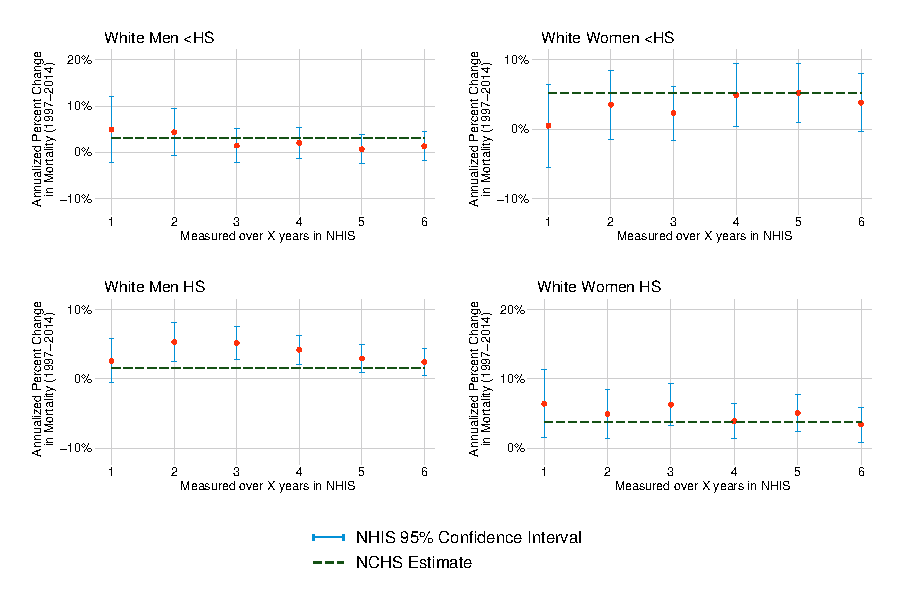
\includegraphics[scale=1.1]{\mortalitypath/ests_yline} \\
  \end{center}
\end{figure}
\scriptsize{The figure compares estimates of annualized mortality
  change in the National Health Interview Survey (NHIS) with vital
  statistics data from the NCHS, used in the body of the paper. The
  annualized change in the mortality rate from 1997--99 to 2015 according to
  NHCS (vital statistics data) is indicated by the dashed green
  line. The six different points for each panel reflect annualized
  mortality changes in the NHIS based on measurement of 1-year
  mortality, 2-year mortality, 3-year mortality, and so on. 1-year
  mortality is reported in the NHIS using 1997--1999 as a base period
  and comparing to participants interviewed in 2014 with mortality followup to 2015. 2-year
  mortality change is reported from 1997--1999 and comparing to 2013 participants,
  and so on. These different estimates are
  nevertheless comparable because the mortality change
  estimates are annualized. Standard errors are calculated for the
  NHIS using NHIS sample weights.}

\begin{figure}[H]
  \caption{Change in Self-Reported Health Status (NHIS, 1997--2015)}
  \label{fig:nhis_health}
  \begin{center}
    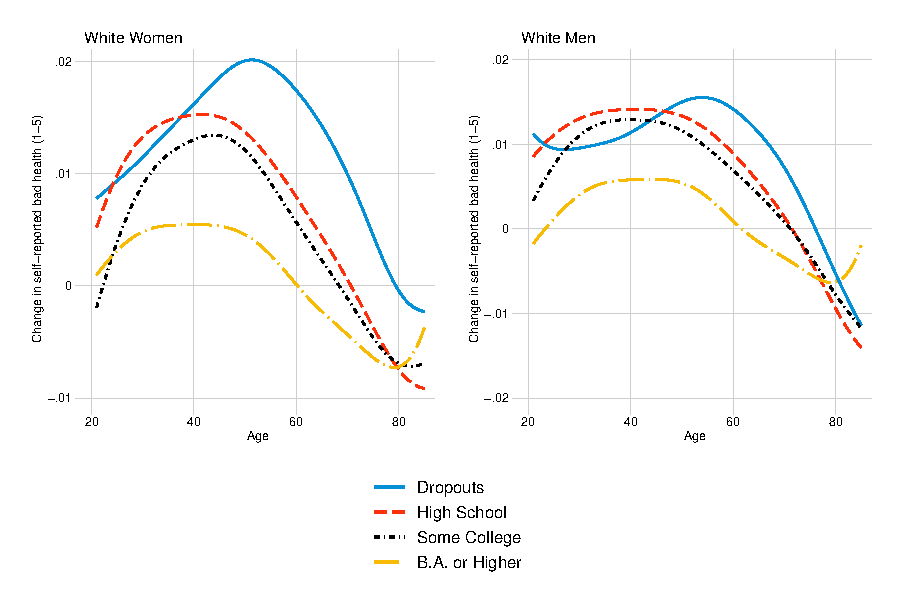
\includegraphics[scale=1.1]{\mortalitypath/lowess_sex_both} \\
  \end{center}
\end{figure}
\scriptsize{The figure shows a lowess fit to the annualized change in
  self-reported health from 1997 to 2015 at each age, according the
  NHIS. Self-reported health status is on a five point scale, where
  one represents the best health and five represents the worst.  We
  calculate annualized change for each age cohort / education group by
  regressing self-reported health status on a year variable. We then
  plot the year coefficients for each age/education group using a
  lowess smoother to minimize noise across single-year age
  cohorts. The series therefore shows the predicted change in
  self-reported health for an individual in a given age, gender and
  education group.}





\clearpage
\subsection{Measurement Error in Education} 
\label{sec:app_ed_error} 
\normalsize This subsection further explores the possibility that measurement error in education biases the main finding of rising mortality among the least educated whites. High school graduation rates on death certificates are thought to be inflated on average, though higher education levels appear to be reported accurately \citep{Sorlie1996}.  There is no evidence that this bias has changed during the sample period, but (as discussed in Appendix~\ref{sec:app_cps_cohorts}) if overreporting of high school completion on death certificates (but not in the CPS) were to decline over time, it would cause mortality change among high school dropouts to biased upward.

For measurement error to explain the rising mortality among dropouts described in this paper, it would need to be the case: (i) that the measurement error in education changes substantially during the sample period; (ii) that measurement error changes differentially for deaths of deaths of despair and deaths in other categories, at different ages, but changes considerably less for deaths of despair; and (iii) that measurement error has declined dramatically for non-Hispanic whites, but has changed only minimally for blacks. Misreporting rates would have to differ substantially across age groups as well---for example, we find that dropouts account for nearly all mortality gain among 50--54-year-olds white women, but that rising mortality is equally distributed among dropouts and high school graduates among 25--29-year-old white women.  

In contrast, if white respondents were increasingly inflating their education in the CPS, we would expect a uniform increase in mortality from all causes, across all ages, which is not remotely what we find. Note also that other researchers have noted rising health disparities between dropouts and high school graduates, in datasets where misreporting of education is unlikely to be a concern \citep{Montez2011}.

We show here that even if one treats the distinction between dropouts and high school graduates as unreliable, the central finding of rising mortality among the least educated remains clear. To show this, we combine dropouts and high school graduates into a single education group, and we estimate mortality change for three constant education percentile bins: (i) percentiles 0-45 (corresponding approximately to dropouts \textit{and} high school graduates in in the middle of the sample period; (ii) percentiles 45-70; and (iii) percentiles 70-100.  Figure~\ref{fig:causes_3ed} shows estimates of mortality change from 1992--94 to 2016--18 for these three groups. We continue to find a dramatic rise in mortality among whites at the bottom of education distribution, though we have defined the bottom more broadly here.  We find that mortality among the bottom 45\% of the education distribution rises over 50\% for white women below 45, rises 0--50\% for women 40-59, and is flat at older ages. Mortality among white men in the bottom 45\% is rising for age groups below 60.

In short, we find significant increases in mortality disparities by education even when we pool high school graduates and high school dropouts.  However, by ignoring the distinction between dropouts and high school graduates, we miss the important difference in causes of death noted in Figure~\ref{fig:mort_causes}---mortality increases outside of the very bottom of the distribution are driven primarily by deaths of despair, but mortality increases in the bottom 10\% are driven by a multitude of causes. Absent evidence that measurement error in death records has changed substantially during the sample period, rising mortality among the least educated 10\% of the population should be taken seriously.

%%%%%%%%%%%%%%%%%%%%%%%%%%%%%%%%%%%%%%%%%%%%%%%%%
% Figure: Causes of Death -- 3 Education Groups %
%%%%%%%%%%%%%%%%%%%%%%%%%%%%%%%%%%%%%%%%%%%%%%%%%
\begin{figure}[H]
  \caption{Change in non-Hispanic White Mortality: 3 Education Groups}
%  \thispagestyle{empty}
  \label{fig:causes_3ed}
  
  \begin{center}
    \vspace{-.6cm} Panel A: Non-Hispanic White Women
  \end{center}
%  \vspace{-1.4cm}
  \begin{center}
    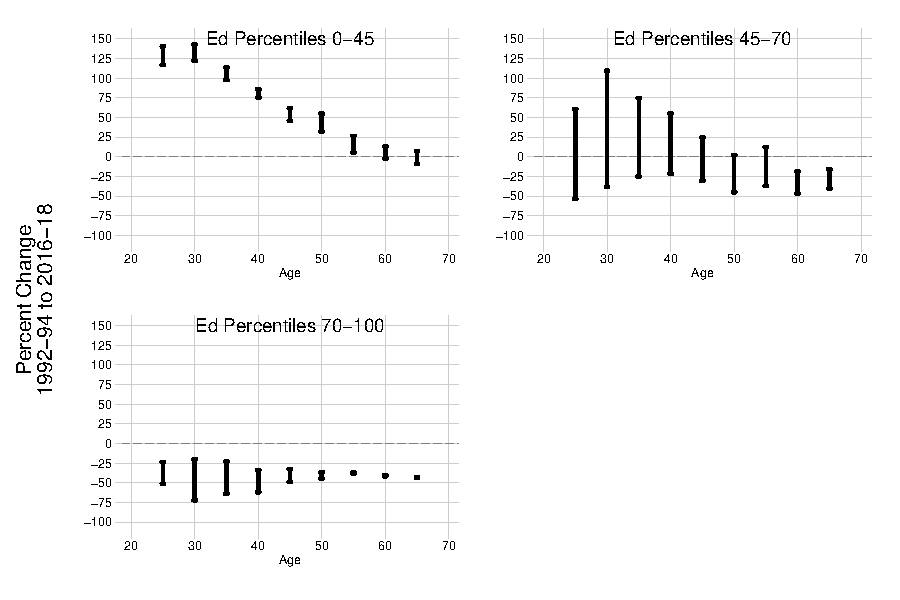
\includegraphics[scale=0.78]{\mortalitypath/causes-ed3-2} &
  \end{center}
  
  \begin{center}
    \vspace{-.6cm} Panel B: Non-Hispanic White Men
  \end{center}
%  \vspace{-1.4cm}
  \begin{center}
    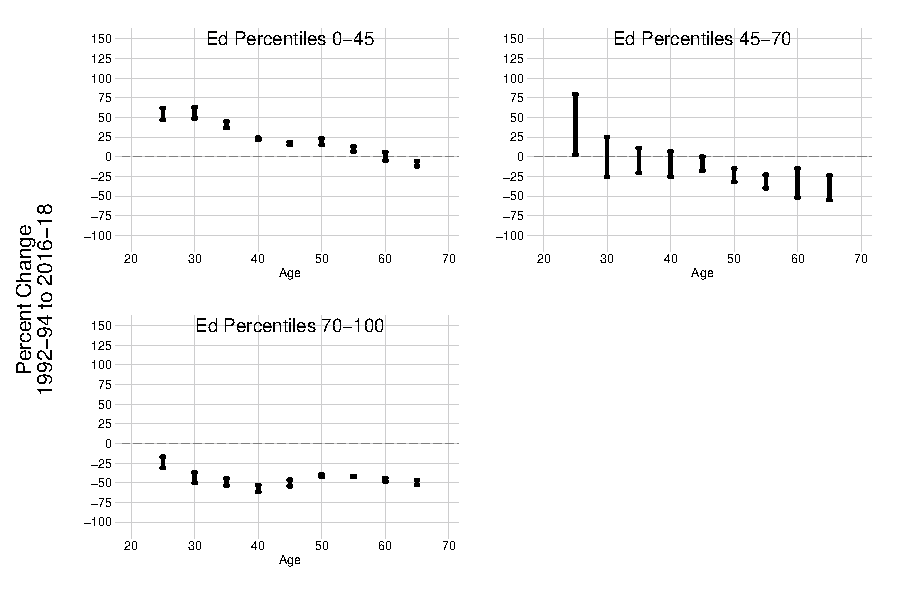
\includegraphics[scale=0.78]{\mortalitypath/causes-ed3-1} \\
  \end{center}
\end{figure}
% \vspace{-1cm}
\tiny{ Note: The graph shows changes in mortality by age, sex, race, and constant percentile education bin. The figure is analogous to Figure \ref{fig:mort_main}, but with the bottom two education categories (percentiles 0--10 and 10--45) pooled into a single category covering percentiles 0--45.  The lines show the bounded set containing the percentage change in the mortality rate from 1992--1994 to 2016--2018 for the given group. Bounds are calculated following Section~\ref{sec:method}. Sources: CPS, NCHS.}


\end{appendix}

\end{document}
